% two-column article ---------------------------------------------------------
%\documentclass[10pt,a4, twocolumn, openright]{article}
% two-column article ---------------------------------------------------------
\documentclass[12pt]{article}

% load standard packages -----------------------------------------------------
\usepackage{amssymb,amsmath,amsfonts,eurosym,geometry,ulem,graphicx,color,sectsty,comment,footmisc,pdflscape,subfigure,array, booktabs}
\usepackage{microtype}
\usepackage{fancyhdr}
\usepackage{threeparttable}
\usepackage{balance}
\usepackage{lettrine}
\usepackage{type1cm}
\usepackage{subfigure}
%\usepackage{bbm}
\usepackage{multirow}
\usepackage{chngcntr}
\usepackage{multicol}
\usepackage{xr}
\usepackage{appendix}
\usepackage{rotating} % Rotating table
\usepackage{tabularx}
\usepackage{booktabs}
\usepackage{dcolumn}

% load packages with special options -----------------------------------------
% natbib package with superscript in-text citations
\usepackage[super,numbers,sort&compress]{natbib}

% gemometry
\geometry{left=1.0in,right=1.0in,top=1.0in,bottom=1.0in,twoside,bindingoffset=0mm}

% set spaces
\usepackage[onehalfspacing]{setspace}

% special colors
\usepackage[dvipsnames, table]{xcolor}

% package for framed boxes
\usepackage[linewidth=3pt]{mdframed}

% captions on top and in sans-serif font for floats
\usepackage[capposition=top, font=sf, capbesideposition=outside,capbesidesep=quad]{floatrow}
\usepackage{adjustbox}

% captions in sans-serif font for caption package
\usepackage[font=sf, singlelinecheck = false]{caption}

% define new commands --------------------------------------------------------
% define new column types for tables
\newcolumntype{P}[1]{>{\centering\arraybackslash}p{#1}}
\newcolumntype{L}[1]{>{\raggedright\let\newline\\arraybackslash\hspace{0pt}}m{#1}}
\newcolumntype{C}[1]{>{\centering\let\newline\\arraybackslash\hspace{0pt}}m{#1}}
\newcolumntype{R}[1]{>{\raggedleft\let\newline\\arraybackslash\hspace{0pt}}m{#1}}

% change number symbol for references in reference list
\makeatletter
\renewcommand\@biblabel[1]{#1.}
\makeatother

% special table cell
\newcommand{\specialcell}[2][c]{%
	\begin{tabular}[#1]{@{}c@{}}#2\end{tabular}}

% define some reasonable margins.
\setlength{\textwidth}{6.6in}
\setlength{\textheight}{8.8in}
\setlength{\topmargin}{-0.1in}
\setlength{\oddsidemargin}{0in}
\setlength{\parskip}{1mm}

% symbol in the tables
\def\sym#1{\ifmmode^{#1}\else\(^{#1}\)\fi}

% what does this do?
\setlength{\floatsep}{5.0pt plus 2.0pt minus 2.0pt}

% for tables
\newcolumntype{x}[1]{%
	>{\centering\hspace{0pt}}p{#1}}%

% define color pastelgray
\definecolor{pastelgray}{rgb}{0.81, 0.81, 0.77}

% change displayed title for reference list
\renewcommand{\refname}{\large  \textbf{\textsf{REFERENCES}}}

% new command for the UZH logo.
\newcommand*{\plogo}{\includegraphics{uzh_logo_e_pos}}

% define new sepline
\newlength{\seplinewidth}
\newlength{\seplinesep}
\setlength{\seplinewidth}{1mm}
\setlength{\seplinesep}{2mm}
\colorlet{sepline}{NavyBlue}
\newcommand*{\sepline}{%
	\par
	\vspace{\dimexpr\seplinesep+.5\parskip}%
	\cleaders\vbox{%
		\begingroup % because of color
		\color{sepline}%
		\hrule width\linewidth height\seplinewidth
		\endgroup
	}\vskip\seplinewidth
	\vspace{\dimexpr\seplinesep-.5\parskip}%
}



% make sure hyperref package is loaded last
\usepackage[colorlinks=true,linkcolor=blue,urlcolor=blue,anchorcolor=blue,citecolor=blue]{hyperref}


%% load supplement for cross-referencing tables and figures
%\externaldocument[sup_]{Appendix}

\begin{document}

\title{
Genetics and Health Insurance: How Genes and Insurance Status Affect Smoking Decisions after Health Shocks
%Genetics and Moral Hazard: health shock when uninsured 
}

\author{Pietro Biroli, Laura Zwyssig}

%\abstract{
%The determinants of healthy behaviors are complex and multifaceted, and include both biological factors, such as genetic predispositions, as well as environmental factors, such as financial liquidity and health insurance status. We show how the choice of smoking after a serious health shock is jointly determined by the interaction between these biological and environmental components. We find that genetic predispositions can offset the financial incentives for smoking cessation. These results suggest that genetic heterogeneity is a factor that should be considered when evaluating the importance of health insurance policies.
%}

\date{\today \\ PRELIMINARY, PLEASE DO NOT CITE}

\maketitle

\normalsize
\begin{mdframed}[backgroundcolor=black!6,linecolor=NavyBlue,leftline=false,rightline=false,bottomline=false, topline=false]
\textsf{\begin{flushleft} \small
\vspace{-5mm}\textbf{\textcolor{NavyBlue}{IMPORTANCE}}
Smoking is the leading preventable cause of death in the United States. Experiencing an adverse health shock can serve as an impetus for cessation. Whether this shock can translate into actual behavior change depends on both the insurance status at the time of the shock as well as a genetic predisposition for smoking.
\noindent\textcolor{white}{\rule{16cm}{0.5mm}}
%
\textbf{\textcolor{NavyBlue}{OBJECTIVE}}
To understand how the smoking response to a health shock varies depending on health insurance (financial risk) and genetic predisposition for smoking (genetic risk).
\noindent\textcolor{white}{\rule{16cm}{0.5mm}}
%
\textbf{\textcolor{NavyBlue}{DESIGN, SETTING, AND PARTICIPANTS}}
Longitudinal study of 3,757 adults in the nationally representative Health and Retirement Study (HRS) who are between 60 and 70 years old, born between 1923 and 1953, observed between 1992 and 2015. Ordinary least squares regression is used to estimate the effect of health shocks for different levels of financial risk exposure and different genetic groups. The differential timing of health shocks before or after the age-based Medicare eligibility threshold for previously uninsured individuals is leveraged to estimate the causal effect of health insurance on behavior change in different genetic groups.
\noindent\textcolor{white}{\rule{16cm}{0.5mm}}
%
\textbf{\textcolor{NavyBlue}{EXPOSURES}}
Experiencing a cardiovascular health shock (heart attack, coronary heart disease, angina, congestive heart failure, other heart problems, stroke, or transient ischemic attack), being uninsured prior to becoming eligible for Medicare at age 65, and a measure for high or low genetic risk for smoking based on a polygenic risk score (PGS) for regular smoking.
\noindent\textcolor{white}{\rule{16cm}{0.5mm}}
%
\textbf{\textcolor{NavyBlue}{MAIN OUTCOMES AND MEASURES}} Self-reported current smoking status, and smoking cessation rates.
\noindent\textcolor{white}{\rule{16cm}{0.5mm}}
%
\textbf{\textcolor{NavyBlue}{RESULTS}}
For low-genetic-risk individuals (n = 1,883; 887 female; 513 baseline smokers), suffering a health shock while being uninsured decreases the probability of smoking by 32 percentage points (95\% CI, -0.58 to -0.06), conditional on baseline characteristics. The effect of the same health shock experienced after age 65 is a 7 percentage point increase in the smoking probability (95\% CI, 0.03 to 0.12), showing that Medicare eligibility fully neutralized the reduction in smoking following the health shock (difference: 40 percentage points, 95\% CI, 0.13 to 0.67). For high-genetic-risk individuals (n = 1,874; 964 female; 528 baseline smokers), having a health shock does not significantly affect the probability of smoking, independent of the timing (effect when uninsured: -1 percentage point, 95\% CI,  -0.31 to 0.28; effect when eligible for Medicare: -12 percentage points, 95\% CI, -0.32 to 0.09; difference: -11 percentage points, 95\% CI, -0.46 to 0.25). The difference in the effect of Medicare eligibility on the smoking response to a health shock between the 2 genetic groups is 50 percentage points (95\% CI, -0.94 to -0.06).
\noindent\textcolor{white}{\rule{16cm}{0.5mm}}
%
\textbf{\textcolor{NavyBlue}{CONCLUSIONS AND RELEVANCE}}
The determinants of healthy behaviors are complex and multifaceted, and include both biological factors, such as genetic predispositions, as well as environmental factors, such as financial liquidity and health insurance status.
%Buffering (some of) the financial costs of illness, Medicare eligibility decreased the probability of smoking cessation after a health shock in individuals with a low genetic predisposition for smoking. This adverse side effect of Medicare eligibility is not observable in those with a high genetic predisposition for smoking, where the health shock had no visible effect on the smoking probability regardless of the financial risk.
We show how the choice of smoking after a serious health shock is jointly determined by the interaction between these biological and environmental components. We find that genetic predispositions can offset the financial incentives for smoking cessation.
These results suggest that genetic heterogeneity is a factor that should be considered when evaluating the importance of health insurance policies.
\end{flushleft}
}
\end{mdframed}


\setcounter{page}{1}

\pagebreak \newpage


\singlespacing

%\twocolumn


%%%%%%%%%%%%%%%%%%%%% INTRODUCTION %%%%%%%%%%%%%%%%%%%%%%%%%%%%%%%%%%%%%%%%%%%
\lettrine[lines=3,lraise=0.01, nindent=0em, slope=0em]{\textcolor{NavyBlue}{\textsf{C}}}{}hronic diseases and health care costs caused by tobacco use are estimated to be one of the biggest health challenges in industrialized countries, and have rapidly increased in importance in the developing world.\cite{USDHHS2014,Goodchild2018} In the US, smoking is estimated to cause more than 400,000 premature deaths annually,\cite{Ma2018} and the economic costs of smoking-related illness amount to around \$300 billion each year, including almost \$170 billion for direct medical care and an additional \$156 billion in lost productivity.\cite{USDHHS2014, Xu2015} Both the health burden from smoking-related illness as well as the economic burden for an already strained health care system have made it a priority to understand what factors affect individuals' smoking decisions, and how health care can effectively encourage cessation.

One factor that has been associated with a reduction in tobacco consumption is health insurance coverage\cite{Richards2014,Marti2017}, especially after experiencing a severe smoking-related health shock, like the onset of a cardiovascular illness.\cite{Clark2002,Falba2005,Khwaja2006learn,Keenan2009,Sundmacher2012}
%The extent to which smoking behavior is improved after a health shock depends, among other things, on the financial cost the individual is faced with after the shock.\cite{Richards2014,Marti2017}
Alleviating the financial burden of health care costs, health insurance can have the unintended side effect of preventing beneficial behavior changes that would have taken place if the individuals were fully responsible for the financial consequences of poor health.\cite{Marti2017} This adverse incentive created by health insurance is a typical example of the concept economists call ``moral hazard'': the notion that individuals change their behavior in an undesired way, because the consequences of their actions are not (fully) borne by themselves.\cite{Einav2018,Zweifel2000}

Another factor that is tightly linked to smoking behavior is genetic makeup. Studies using identical and fraternal twins have estimated that genetic factors can explain around 30\% to 85\% of the variance of regular smoking.\cite{Heath1993, Sullivan1999, Hall2002, Li2003, Boardman2010} In recent years, significant progress has been made in identifying genetic variants associated with susceptibility for smoking.\cite{Liu2010,Thorgeirsson2008,Thorgeirsson2010,TAG2010,Liu2018gwas} This development, together with an increased availability of genetic measures in large representative surveys, allows for a better understanding of how genetics can interact with other factors in determining smoking behavior.

%%TODO: This first sentence is a little bit too general


This study is the first to show how genetic and financial risks jointly influence individual choices of health behavior. Specifically, we show that moral hazard stemming from health insurance (financial risk) interacts with genetic predisposition for smoking (genetic risk) in determining the probability of smoking cessation following a health shock. Using data from the Health and Retirement Study (HRS), a longitudinal population-based study of elder Americans, we estimated how experiencing a health shock between survey waves affected the smoking probability of individuals with different coverage levels and genetic predispositions for smoking.

To cleanly identify this interaction effect between genes and the environment, we leverage a key feature of the US health insurance system: Medicare, which provides public health insurance to all US citizens older than 65. Before the introduction of the Affordable Care Act,\cite{Obama2016} a significant fraction of the population younger than 65 was still uninsured.\cite{Cohen2009,Barnett2016} Exploiting the differential timing of health shocks before or after the Medicare-eligibility age of 65 for previously uninsured individuals, we estimate that Medicare eligibility reduced smoking cessation rates after a health shock, but only for those individuals with a low genetic propensity to smoking. Comparing this effect between individuals with a high versus a low genetic predisposition for smoking allows for an assessment of how the moral hazard problem found in previous research interacts with genetic risk.

%%TODO: find better references for personalized medicine

Our results highlight the importance of considering genetic predisposition when evaluating behavioral responses to health insurance coverage.\cite{Brock1993,Morrison2005} Genetic predispositions can curb the negative behavioral consequences and the moral hazard associated with changes health insurance status. In the era of genomics and personalized medicine,\cite{Khera2018,Torkamani2018,Schork2018,Ritz2017} an individual genetic makeup can be a factor not only in the treatment they receive, but also in their response to insurance coverage.

%%%%%%%%%%%%%%%%%%%%% KEY POINTS %%%%%%%%%%%%%%%%%%%%%%%%%%%%%%%%%%%%%%%%%%%%%
\begin{mdframed}[backgroundcolor=black!6,linecolor=NavyBlue,leftline=false,rightline=false,bottomline=false]
	\textbf{\textsf{KEY POINTS}} \vspace{1.5mm} \footnotesize

	\noindent \textsf{\textbf{\textcolor{NavyBlue}{Question}}
	How does the smoking response to a health shock vary with health insurance (financial risk) and genetic predisposition for smoking (genetic risk)?
	}

	\vspace{1mm}

	\noindent \textsf{\textbf{\textcolor{NavyBlue}{Findings}}
	In a sample of US adults aged between 60 and 70 years, experiencing a health shock while uninsured decreases the smoking probability in individuals with a low genetic risk for smoking. Medicare eligibility after age 65, and hence a lower exposure to the financial costs of illness, fully neutralized this cessation effect. For those with a high genetic risk for smoking, experiencing a health shock does not lead to any visible behavior changes, regardless of insurance status.
	}

	\vspace{1mm}

	\noindent \textsf{\textbf{\textcolor{NavyBlue}{Meaning}} A high genetic predisposition for smoking may overpower both health-related and financial motives for cessation after a health shock.
	}
\end{mdframed}

%%%%%%%%%%%%%%%%%%%%% KEY POINTS %%%%%%%%%%%%%%%%%%%%%%%%%%%%%%%%%%%%%%%%%%%%%


%%%%%%%%%%%%%%%%%%%%% METHODS %%%%%%%%%%%%%%%%%%%%%%%%%%%%%%%%%%%%%%%%%%%%%%%%
\sepline
\vspace{1mm}
\noindent \textbf{\large \textsf{METHODS} }
\vspace{1mm}

\noindent \textbf{\textsf{\textcolor{NavyBlue}{Analytic Sample}}}

\noindent The HRS is a nationally representative longitudinal household survey initiated in 1992 among US citizens aged 50 and older, followed for 12 waves over 22 years (response rates between 80\% and 90\% \cite{HRSResponseRate}).\footnote{
Every 6 years, a new 6-year birth cohort of participants is enrolled.\cite{HRS21stCentury}
It is sponsored by the National Institute on Aging (grant number NIA U01AG009740) and is conducted by the University of Michigan.\cite{HRSWebsite}
The first core interview with every participant is conducted face-to-face, and all follow-up interviews are either face-to-face or over the phone.\cite{HRS21stCentury}
}
This study uses data from the publicly available RAND HRS file (version P)\cite{HRSRAND} -- an easy-to-use longitudinal data set based on the HRS data -- as well as the publicly available initial release of the HRS polygenic scores data.\cite{HRSPGENSCORE} These scores are based on DNA samples collected in enhanced face-to-face interviews, for which a random subset of HRS households is selected to participate in 2006, 2008, and 2010. Saliva samples are collected and genotyped for more than 15,000 participants.\cite{HRSPGenscore2017} More information on the DNA extraction and genotyping process is provided in Section \ref*{supsec:dna_genotyping} in the Supplement.

The analytic sample used in this study consists of the 5,541 HRS respondents who are between 60 and 70 years of age at the time of the interview, ever-smokers at baseline (their first observation), observed in at least 2 different time periods, and genetically of European descent. Additionally, the sample is restricted to observations with non-missing values for smoking status, polygenic risk score (PGS) for regular smoking, insurance status, and the occurrence of heart conditions or strokes (see Section \ref*{supsec:analytic_sample} in the Supplement for more information on the construction of the analytic sample). The age restriction imposed on the study sample increases comparability between those experiencing a health shock before or after age 65. The restriction imposed on genetic ancestry increases the similarity with the genetic profile of the discovery sample used in the genome-wide association study\cite{TAG2010} (GWAS) that informed the weights for the single nucleotide polymorphisms (SNPs) used for calculating the PGSs.\cite{HRSPGenscore2017}
In addition, we exclude respondents who reported the onset of a cardiovascular illness since the last survey wave when interviewed at ages 65 or 66. Since HRS surveys are only conducted every 2 years, it is not possible to determine Medicare eligibility status at the time of the health shock for these individuals.



\vspace{5mm}
\noindent \textbf{\textsf{\textcolor{NavyBlue}{Outcome and Exposure Variables}}}

\noindent \textsf{Smoking status.} The outcome of interest is a self-reported binary indicator for current smoking status, where smoking refers to having smoked more than 100 cigarettes throughout one's life (ever-smoker) and smoking at the time of the survey. We also calculate cessation rates, defined as smoking in the previous but not in the current wave. \\

\noindent \textsf{Health shocks.} Following previous studies,\cite{Falba2005,Keenan2009,Khwaja2006spouse,Khwaja2006learn,Smith2001} this analysis consideres acute cardiovascular conditions. These conditions have strong links to tobacco use, have a relatively high incidence among older adults, and are likely to require an immediate and intensive use of costly medical services.\cite{Thorpe2004,Teo2006,Lloyd-Jones2010} Additionally, they can occur again and again for the same individual and thereby incentivize improvements in health behaviors to prevent reoccurrence.

This study uses a binary health shock indicator. It is set to ``1'' if a respondent is diagnosed with a new cardiovascular condition during the time since the last HRS survey, but does not have a history of cardiovascular disease prior to this diagnosis. Cardiovascular conditions include either a heart problem (heart attack, coronary heart disease, angina, congestive heart failure, or other heart problems) or a stroke (or transient ischemic attack). The exact timing of the health shock within the past 2 years since the last interview is not observed, and the diagnoses are all self-reported.\\

\noindent \textsf{Medicare eligibility status.} An indicator variable for Medicare eligibility status is set to ``1'' for individuals aged 65 years or above in a given HRS wave.\\


\noindent \textsf{Pre-65 uninsured status.} HRS respondents are classified as uninsured in a given survey wave if they reported not being covered by any health insurance plan. A binary variable is defined for pre-65 uninsured status that takes the value ``1'' if a respondent is persistently uninsured in every observation before the age of 65. \\


\noindent \textsf{Polygenic risk for regular smoking.} HRS provides a polygenic risk score for the smoking phenotype ``regular smoking'' (having smoked more than 100 cigarettes throughout one's life). This score is constructed as a weighted sum of the genotype over the 779,538 SNPs that overlap between the HRS genetic database and a 2010 GWAS meta-analysis conducted by the Tobacco and Genetics Consortium.\cite{TAG2010} Specifically, the scores are calculated as follows:
\begin{align}
PGS_i = \sum_{j=1}^{J} W_j G_{ij},
\end{align}
\normalsize where $G_{ij}$ is the genotype for individual $i$ at SNP $j$, and the weight $W_j$ is the meta-analysis estimated effect size for SNP $j$ (see Section \ref*{supsec:PGS} in the Supplement for more information on the GWAS used for informing SNP weights). The scores have been normalized to have mean zero and standard deviation one.\cite{HRSPGenscore2017}

For the statistical analysis, this PGS is used to split the sample into 2 genetic groups. A high-PGS indicator is defined to take the value ``1'' for individuals with a PGS above the median. Figure \ref*{supfig:PGS} in the Supplement illustrates the relationship between the PGS and smoking behavior in the HRS data. \\

\noindent More information on the construction of all variables used in the analysis can be found in Section \ref*{supsec:outcome_exposure} in the Supplement.


\vspace{5mm}
\noindent \textbf{\textsf{\textcolor{NavyBlue}{Statistical Analysis}}}

\noindent
%We report two sets of results: first of all, we compare the average smoking cessation rates for those who suffer a health shock before and after the age of 65, stratified by high and low genetic propensity. 
%We then run a more sophisticated analysis controlling for age and individual characteristics.
We run a within-person analysis relating smoking rates for those who suffer a health shock before and after the age of 65, stratified by uninsured status and high and low genetic propensity.

This empirical approach follows previous work\cite{Marti2017} and leverages the differential timing of health shocks before or after the age-based Medicare eligibility threshold. The exact timing of the shock (before or after age 65) is arguably both exogenous and unanticipated.
While the probability of experiencing a new cardiovascular illness increases with age,\cite{Lloyd-Jones2010} in the HRS data there is no observable jump (or change in trend) in the percentage of respondents reporting a health shock around the age of 65 (see Section \ref*{supsec:age_pattern_cv} in the Supplement for details). Accounting for the influence of age on the probability of suffering from cardiovascular illness, there is therefore no reason to suspect that respondents experiencing the shock after 65 are systematically different from respondents experiencing the shock before 65. The setting thus provides a good framework for estimating the causal effect of Medicare eligibility on the smoking response to a health shock in individuals who are uninsured before the age of 65.

Conceptually, this design can be thought of as aiming to achieve the following hypothetical comparisons: within both the low-PGS and the high-PGS group, compare 2 ever-smokers with similar characteristics (gender, health insurance trajectory, age, etc.) regarding how their smoking status is affected by experiencing a health shock. The only difference between the 2 individuals is the point in time at which they experience the shock and, hence, their exposure to the financial costs associated with it.

Methodologically, for the second sets of results we use ordinary least squares (OLS) regression to estimate a linear probability model for smoking. Current smoking status ($Y$) is regressed on the full set of interactions between the indicators for the health shock ($shock$), being uninsured pre-65 ($uninsured$), Medicare eligibility ($post65$), and high polygenic risk for smoking ($g$):

\begin{align} \label{regression}
Y_{it}& \thinspace  = \thinspace
				\beta \thinspace shock_{it} + \gamma \thinspace post65_{it} \\
				&+\lambda_1 \thinspace  (shock_{it} \times post65_{it}) \nonumber \\
				&+ \lambda_2 \thinspace (shock_{it} \times uninsured_i) \nonumber \\
				&+\lambda_3  \thinspace (post65_{it} \times uninsured_i) \nonumber \\
				&+ \lambda_4 \thinspace (shock_{it} \times g_i) \nonumber \\
				&+\lambda_5 \thinspace (post65_{it} \times g_i) \nonumber \\
				&+ \delta_1 \thinspace (shock_{it} \times post65_{it} \times uninsured_i) \nonumber \\
				&+ \delta_2 \thinspace (shock_{it} \times uninsured_i \times g_i) \nonumber \\
				&+ \delta_3 \thinspace (shock_{it} \times post65_{it} \times g_i) \nonumber \\
				&+ \delta_4 \thinspace (post65_{it} \times uninsured_i \times g_i) \nonumber\\
				&+ \zeta \thinspace (shock_{it} \times post65_{it} \times uninsured_i \times g_i) \nonumber \\
				&+ \sum_{a=1}^3 \phi_a \thinspace age_{it}^{a} + \eta_i + \tau_t + \varepsilon_{it} \nonumber
\end{align}

Individual fixed effects ($\eta_i$) are included to control for unobserved time-invariant differences between respondents, and time fixed effects ($\tau_t$) to control for time-specific confounders. In addition, the respondent's age in years at the time of the interview ($age$) is added as a covariate. Equation (\ref{regression}) is estimated using heteroskedasticity-robust standard errors that are clustered at the individual level. All statistical analyses in this study are conducted with the software R, version 3.4.2, and various open-source packages.\cite{broom,car,ggplot2,haven,labelled,lmtest,multcomp,plm,plyr,readr,readxl,reshape2,sandwich,scales,stargazer,stringr,tidyverse}



% Table created by stargazer v.5.2 by Marek Hlavac, Harvard University. E-mail: hlavac at fas.harvard.edua
% Date and time: Do, Mai 03, 2018 - 16:44:15
\begin{table}[!h]
	\caption{Descriptive Statistics for the Full Analytic Sample and Stratified by Genetic Group \vspace{-0.3cm}}
	\label{tab:descriptives_full}
	\resizebox{\textwidth}{!}{
		\Large % latex table generated in R 4.0.2 by xtable 1.8-4 package
% 
\begin{tabular}{llll}
  \toprule
\textbf{ } & \textbf{ All } & \textbf{ Low PGS } & \textbf{ High PGS } \\ 
  \midrule
 & Mean (SD) & Mean (SD) & Mean (SD) \\ 
   \midrule
Age (baseline) & 61.17 (1.93) & 61.18 (1.96) & 61.16 (1.92) \\ 
  Smoking PGS & 0.11 (0.99) & -0.96 (0.51) & 0.64 (0.71) \\ 
  No. waves present & 4.44 (1.38) & 4.46 (1.37) & 4.43 (1.39) \\ 
   & \% & \% & \% \\ 
  Female & 50.42 & 46.97 & 52.14 \\ 
  Smoking (baseline) & 29.55 & 27.06 & 30.79 \\ 
  Persistently uninsured & 5.85 & 5.39 & 6.08 \\ 
  CV health shock & 12.44 & 11.82 & 12.74 \\ 
   \midrule
No. of individuals & 5813 & 1929 & 3884 \\ 
  No. Person-year observations & 25800 & 8602 & 17198 \\ 
   \bottomrule
\end{tabular}

	}
		%\begin{tablenote}[para,flushleft]
			\footnotesize
	\begin{flushleft}
	Note: Low PGS: PGS $\leq$ median PGS. High PGS: PGS $>$ median PGS.\\
	P values report significance tests for the difference in means between the genetic groups.\\
	Cessation rates are defined as smoking in the previous but not in the current wave.\\
	Data used: Analytic sample.
	\end{flushleft}
		%\end{tablenote}
\end{table}

The statistical method resembles a difference-in-differences approach, but considers a quadruple difference rather than the usual double difference: we compared the effect of a health shock for those experiencing it before or after Medicare eligibility age, who are either previously uninsured or insured, and who have either a low or high genetic risk for smoking. The subgroup of interest is comprised of those who are uninsured before the age of 65, and for whom Medicare eligibility hence represented a drastic reduction in the financial risk associated with poor health. For this subgroup, which comprises 327 individuals, the comparisons of interest are experiencing the health shock before versus after age 65, and having a low versus a high genetic risk for smoking.

For the group of previously uninsured individuals, we are interested in 3 different types of effects:

First, what is the marginal effect of a health shock on smoking? This effect is calculated for 4 different subgroups, given by the combinations of shock timing (pre- or post-65) and genetic risk (high or low). For each subgroup, the effect is comprised of the sum of all coefficient estimates from Equation (\ref{regression}) that applied for the given group. For example, for previously uninsured individuals who experienced the shock before the age of 65 and who had a low genetic susceptibility for smoking, the effect of the health shock is calculated by summing up the estimates for $\beta$ and $\lambda_2$. If the health shock is instead experienced after 65, the effect of the shock (for the same group of previously uninsured low-PGS individuals) is the sum of the estimates for $\beta$, $\lambda_1$, $\lambda_2$, and $\delta_1$.

Second, what is the causal effect of Medicare eligibility (and hence a change in the financial costs associated with a health shock) on smoking? This effect is calculated using the difference between the pre-65 shock effect and the post-65 shock effect for each of the 2 genetic groups. For the low-PGS group, it is given by the sum of the estimates for $\lambda_1$ and $\delta_1$. For the high-PGS group, it is given by the sum of  $\lambda_1$, $\delta_1$, $\delta_3$, and $\zeta$.

Lastly, to assess how moral hazard is associated with different levels of genetic predisposition for smoking, we ask if and how the effect of Medicare eligibility on the post-shock smoking decision is different between the high- and the low-PGS groups. This effect of having a high genetic predisposition for smoking is comprised of the sum of the estimates for $\delta_3$ and $\zeta$ in Equation (\ref{regression}).




\vspace{5mm}

\noindent \textbf{\textsf{\textcolor{NavyBlue}{Additional Analyses}}}

\noindent We perform a series of additional analyses to test the robustness of my findings. We relax the criteria for inclusion in the pre-65 uninsured group, including respondents who are uninsured in only 75\% or 50\% of all pre-65 observations, and we vary the definition of the high-PGS indicator by using the 45th or 55th percentiles rather than the median as cutoff. Additionally, the age restriction imposed on the analytic sample is relaxed and expanded by up to 5 years at each end. Finally, we also test if results are affected by the sample restriction of excluding HRS respondents for whom Medicare eligibility status at the time of the health shock is unknown (when health shocks are reported at ages 65 or 66).\\


\captionsetup{width = 16.2cm}
% TABLE WITH P VALUE COLUMN
% Table created by stargazer v.5.2 by Marek Hlavac, Harvard University. E-mail: hlavac at fas.harvard.edu
% Date and time: Do, Apr 26, 2018 - 20:20:16
\begin{table*}[!h] \centering
	\caption{Descriptive Statistics for the Subset of the Analytic Sample with a Health Shock, Stratified by Timing of the Shock and Genetic Group}
	\label{tab:descriptive_subgroup}
	%\resizebox{\textwidth}{!}{
	% latex table generated in R 4.0.2 by xtable 1.8-4 package
% 
\begin{tabular}{llll}
  \toprule
\textbf{  } & \textbf{ Low PGS } & \textbf{ High PGS } & \textbf{ P value } \\ 
  \midrule
Shock at ages 60-64 &  &  &  \\ 
   \midrule
 & Mean (SD) & Mean (SD) &  \\ 
  Age (baseline) & 60.49 (0.57) & 60.46 (0.62) & 0.67 \\ 
  Smoking PGS & -0.97 (0.54) & 0.63 (0.68) & 0.00 \\ 
  Years of education & 12.17 (3.44) & 12.15 (3.12) & 0.95 \\ 
  Income (nominal \$ 1000) & 19.61 (27.99) & 18.9 (30.1) & 0.83 \\ 
  No. waves present & 4.65 (1.31) & 4.59 (1.31) & 0.66 \\ 
   & \% & \% &  \\ 
  Female & 48.21 & 45.26 & 0.60 \\ 
  Smoking (baseline) & 30.36 & 37.23 & 0.19 \\ 
  Persistently uninsured & 4.46 & 6.57 & 0.39 \\ 
  Avg. cessation rate (baseline smokers) & 11.95 & 12.09 & 0.96 \\ 
  No. of individuals & 112 & 274 &  \\ 
   \midrule
No. of Person-year individuals & 521 & 1257 &  \\ 
   \midrule
Shock at ages 67-70 &  &  &  \\ 
   & Mean (SD) & Mean (SD) &  \\ 
  Age (baseline) & 61.16 (1.9) & 61.01 (1.22) & 0.44 \\ 
  Smoking PGS & -0.94 (0.48) & 0.76 (0.8) & 0.00 \\ 
  Years of education & 12.73 (3.15) & 12.42 (3.07) & 0.40 \\ 
  Income (nominal \$ 1000) & 17.75 (27.24) & 16.1 (20.41) & 0.58 \\ 
  No. waves present & 5.13 (1.05) & 5.13 (0.75) & 0.99 \\ 
   & \% & \% &  \\ 
  Female & 40.91 & 47.98 & 0.22 \\ 
  Smoking (baseline) & 28.18 & 34.98 & 0.21 \\ 
  Persistently uninsured & 8.18 & 6.28 & 0.54 \\ 
  Avg. cessation rate (baseline smokers) & 9.94 & 10.83 & 0.75 \\ 
   \midrule
No. of individuals & 110 & 223 &  \\ 
  No. of Person-year individuals & 564 & 1143 &  \\ 
  \end{tabular}

	\begin{flushleft}
			\footnotesize
			Pre-65: Health shock since last survey reported at ages 60-64.\\
			Post-65: Health shock since last survey reported at ages 67-70.\\
			P values report significance tests for the difference in means between the shock timing strata.\\
			Low PGS: PGS $\leq$ median PGS. High PGS: PGS $>$ median PGS.\\
			Cessation rates are defined as smoking in the previous but not in the current wave.\\
			Data used: Analytic sample restricted to individuals experiencing a health shock during the observation period.
	\end{flushleft}
	%	}
\end{table*}


%%%%%%%%%%%%%%%%%%%%%%%%%%%%%%%%%%%%%% RESULTS %%%%%%%%%%%%%%%%%%%%%%%%%%%%%%%%%%%%%%%%%%%%%%%%%
\vspace{-0.9mm}
\color{sepline}%
\hrule width\linewidth height\seplinewidth
\vspace{2mm}
%\sepline
\normalsize
\vspace{1mm}
\color{Black}
\noindent \textbf{\large \textsf{RESULTS}}
\vspace{1mm}


\noindent \textbf{\textsf{\textcolor{NavyBlue}{Sample Characteristics}}}

\noindent The first column in Table \ref{tab:descriptives_full} summarizes the analytic sample used for estimation. Average age at baseline is 61.2 years, and an individual is observed for 4.4 waves on average, has 12.4 years of education, and reports an income of \$20,101 per year. 49.8\% of the sample is made up of women, and 29.5\% smokes at baseline. 5.9\% of individuals in the sample are uninsured in all observations before the age of 65, and 12.3\% experience a cardiovascular health shock during the observation period. The full analytic sample consisted of 5.541 individuals (and 24,307 person-year observations). The second and third columns in Table \ref{tab:descriptives_full} describe the sample stratified into the 2 genetic groups. High-PGS respondents are more likely to be uninsured before the age of 65, and included relatively more women compared to the low-PGS respondents.

Table \ref{tab:descriptive_subgroup} displays summary statistics for the subset of the analytic sample that experienced a cardiovascular health shock over the course of the observation period, stratified by timing of the shock (pre-65 versus post-65) and genetic group.\footnote{
This subset of respondents affected by cardiovascular illness during the observed years differed in some characteristics from those unaffected. Table \ref{suptab:descriptives_full} in the Supplement shows a comparison.
}%
Within a genetic group, demographics are mostly similar across the timing strata. However, in both groups, those experiencing the shock after age 65 are on average older at baseline. In the high-PGS group, there are also relatively more women experiencing the shock after the age of 65 than before 65. This is consistent with the general pattern that women experience cardiovascular disease later in life than men.\cite{Lloyd-Jones2010}


%\noindent \textbf{\textsf{\textcolor{NavyBlue}{Average Cessation Rates}}}
%\noindent
%Our main results are already apparent by simply focusing on the average smoking cessation rates of the four groups in our analysis: those who suffer a health shock before or after the age of 65, and those with high or low genetic propensity to smoking. These four averages are reported in Table \ref{tab:descriptive_subgroup} and displayed in Figure \ref{fig:rawcessation}.
%
%In the low-PGS group, the average cessation rate for baseline smokers is significantly smaller among those experiencing the shock while eligible for Medicare ($9.1\%$) than it is for those who had the shock before the age of 65 ($15.2\%$). In the high-PGS group, cessation rates does not differ across the timing strata ($\approx 11\%$).
%
%\captionsetup{width = \columnwidth}
%\begin{figure}[!h]
%	\begin{center}
%	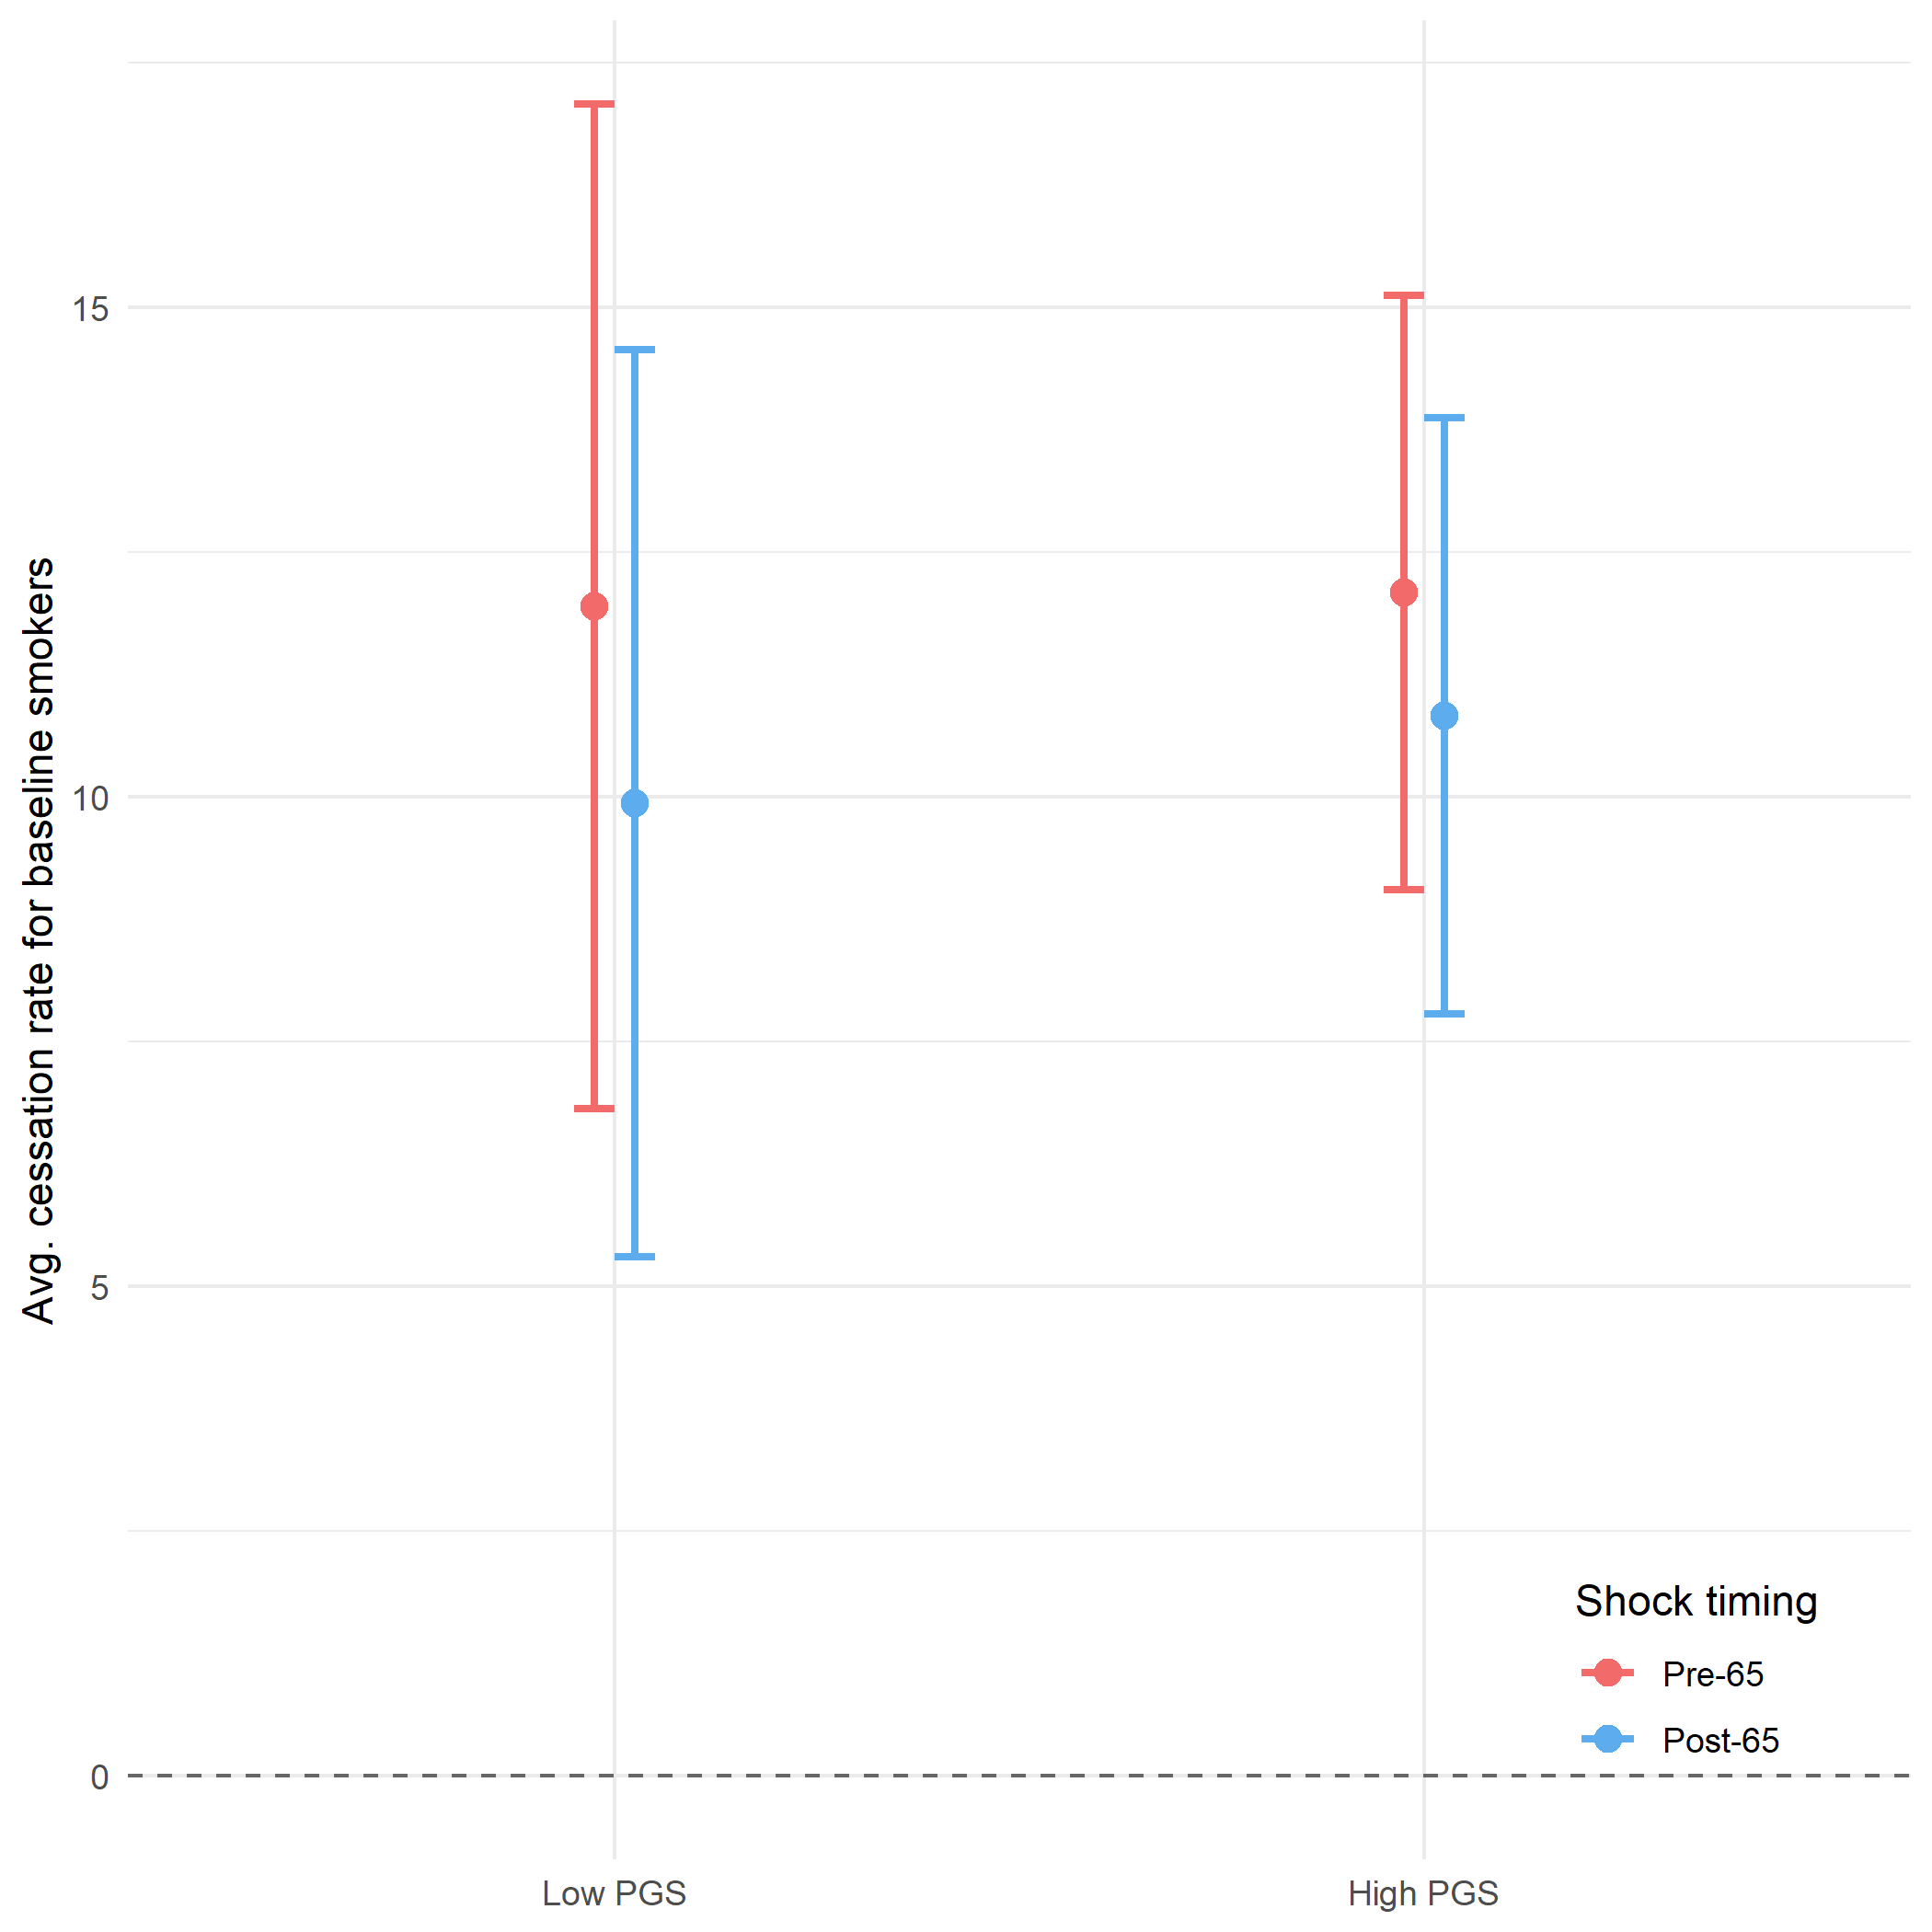
\includegraphics[height=0.8\textheight]{../3_output/cess_rates_graph/graph_6070plot2.png}
%		\caption{Average smoking cessation rate, stratified by timing of the shock and genetic group\vspace{-3mm}
%			\label{fig:rawcessation}}
%		\floatfoot{\vspace{-0.8cm} \\
%			\textsf{Low PGS: PGS $\leq$ median PGS. High PGS: PGS $>$ median PGS.\\ Pre-65: Health shock since last survey reported at ages 60-64.\\
%				Post-65: Health shock since last survey reported at ages 67-70. \\
%				Bars show 95\% confidence intervals. Averages are shown in Table \ref{tab:descriptive_subgroup}. Data used: Analytic sample.}}
%	\end{center}
%\end{figure}



\noindent \textbf{\textsf{\textcolor{NavyBlue}{Estimation Results}}}

%%TODO guide the reader more
\noindent Although indicative of the main patterns in the data, the above results could be confounded by the fact that health shocks are more likely to occur at later ages, or other individual characteristics. We therefore run a regression analysis that controls for these potential confounders.

Regression results are presented in Table \ref{tab:reg_results}. Based on these estimates, Figure \ref{fig:shock_effects} visualizes the marginal effect of a health shock on the smoking probability for individuals who are uninsured before the age of 65 -- the subgroup of interest -- for the 4 combinations of shock timing and genetic risk. For individuals who are genetically less susceptible for smoking, experiencing a cardiovascular health shock while uninsured significantly reduces the probability of smoking by 32 percentage points. For the subgroup of uninsured individuals with a high genetic predisposition for smoking, the estimated effect of the health shock is not statistically significantly different from 0. A health shock experienced after the age of Medicare eligibility, for previously uninsured individuals, increased the smoking probability in the low-PGS group by 7 percentage points. While this effect is relatively small compared to the magnitude of the effect of a pre-65 health shock, there is no immediate intuitive explanation for the observed direction. For individuals with a high genetic risk for smoking, the estimated effect of the health shock is again not statistically significantly different from 0 when the shock is experienced after the age of 65.

These 4 effects -- constituting the first type of effect that is of interest in this study -- are listed in Panel A of Table \ref{tab:main_effects}. Panels B and C of Table \ref{tab:main_effects} illustrate the other 2 types of effects -- the effect of Medicare eligibility on the smoking response, and the difference in this effect between the 2 genetic groups. This provides evidence of a strong gene-environment interaction effect.


Panel B of Table \ref{tab:main_effects} shows that Medicare eligibility after age 65 counteracted the effect of the health shock in the low-PGS group by 40 percentage points, increasing it from the pre-65 32-percentage-point reduction in the smoking probability to the 7-percentage-point increase. In the high-PGS group, no statistically significant effect of Medicare eligibility on the smoking response is found. The estimated causal effect of Medicare eligibility differed significantly between individuals with a high or a low genetic risk for smoking. As shown in Panel C of Table \ref{tab:main_effects}, the difference in the effect between the 2 genetic groups amounted to 50 percentage points.


Altogether, this implies that Medicare eligibility had a stronger impact on the post-shock smoking probability in the low-PGS group than in the high-PGS group. In the low-PGS group, the effect of Medicare eligibility is unfavorable in terms of health behaviors, indicating problems of moral hazard in this subgroup.

Additional analyses confirm that these dynamics are robust to changes in the definition of the high-PGS indicator (having a PGS above the 45th or 55th percentiles instead of the median), the definition of the pre-65 uninsured status indicator (uninsured in 75\% of all pre-65 observations instead of 100\%), and the age range used for the analytic sample (59-71, 58-72, 57-73, 56-74, or 55-75 instead of 60-70). Relaxing the definition of the uninsured indicator to include respondents uninsured in a minimum of 50\% of pre-65 observations leaves the directions of the effects unchanged, but the magnitudes are smaller and statistical significance is lost. Furthermore, the findings of this study do not depend on the exclusion of HRS respondents for whom Medicare eligibility status at the time of the shock is unknown (when health shocks are reported at ages 65 or 66). Estimation results for all robustness checks are shown in Section \ref*{supsec: robustness} in the Supplement.

A possible concern with the design of this study is that there may be other factors happening around the age of 65 that affect smoking behavior after health shocks and which this analysis could not account for, such as entry into retirement. It is, however, hard to reconcile this alternative interpretation with the findings: If retirement rather than insurance status were to cause the difference between the effects of a pre- vs. post-65 health shock in the low-PGS group, one could expect to also see an effect for those insured before the age of 65. As Table \ref{tab:reg_results} shows, however, whether the shock took place before or after the age of 65 does not impact its effect on the smoking probability in the pre-65 insured group (the estimated coefficient on the \textsf{shock x post-65} interaction is close to 0 and not statistically significant).\\ \vspace{-2mm}


\captionsetup{width = 9cm}
% Table created by stargazer v.5.2 by Marek Hlavac, Harvard University. E-mail: hlavac at fas.harvard.edu
% Date and time: Do, Apr 26, 2018 - 19:53:30
\begin{table}[h] \centering
	\caption{Coefficients from Estimating the Linear Probability Model in Equation (\ref{regression}) Using OLS\vspace{-0.4cm}}
	\label{tab:reg_results}
	\input{../3_output/OLSresults/linprob.tex}
	\begin{flushleft}
	 Robust standard errors in parentheses are clustered at the individual level. \\
	Regression included individual and year fixed effects.\\
	Data used: Analytic sample.
	\end{flushleft}
\end{table}



\captionsetup{width = \columnwidth}
\begin{figure}[!h]
	\begin{center}
		\includegraphics[width=\textwidth]{../3_output/shock_effects/main_6070_100_cvinverse_plot.png}
		\caption{Marginal Effect of a Health Shock on the Smoking Probability in the Pre-65 Uninsured Subgroup, Stratified by Timing of the Shock and Genetic Group\vspace{-3mm}
			\label{fig:shock_effects}}
		\floatfoot{\vspace{-0.8cm} \\
			\textsf{Low PGS: PGS $\leq$ median PGS. High PGS: PGS $>$ median PGS.\\ Pre-65: Health shock since last survey reported at ages 60-64.\\
				Post-65: Health shock since last survey reported at ages 67-70. \\
				Bars show 95\% confidence intervals. Estimates and standard errors are shown in Panel A of Table \ref{tab:main_effects}. Data used: Analytic sample.}}
	\end{center}
\end{figure}




\captionsetup{width = 9cm}
% Table created by stargazer v.5.2 by Marek Hlavac, Harvard University. E-mail: hlavac at fas.harvard.edu
% Date and time: Do, Apr 26, 2018 - 12:58:22
\begin{table*}[h]
	\caption{Summary of Statistical Results for the Pre-65 Uninsured Subgroup, Stratified by Timing of the Shock and Genetic Group}
	\label{tab:main_effects}
	%\resizebox{7.5cm}{!}{
	% latex table generated in R 4.0.2 by xtable 1.8-4 package
% 
\begin{tabular}{lll}
  \toprule
  \multicolumn{3}{c}{ \textbf{Effect of health shock on smoking probability}} \\
 \midrule
 & Low PGS & High PGS \\ 
   \midrule
Pre 65 & -0.165** & -0.108 \\ 
   & (0.069) & (0.083) \\ 
  Post 65 & 0.09*** & -0.13 \\ 
   & (0.026) & (0.089) \\ 
   \toprule \multicolumn{3}{c}{ \textbf{Effect of health insurance on effect of health shock}} \\
 \midrule
 & Low PGS & High PGS \\ 
   \midrule
Post 65 - Pre 65 & 0.256*** & -0.023 \\ 
   & (0.079) & (0.121) \\ 
   \toprule \multicolumn{3}{c}{ \textbf{Differential effect of health insurance by genetic group}} \\
 \midrule
 & High PGS  & - low PGS \\ 
   \midrule
Post 65 - Pre 65 & -0.279* &  \\ 
   & (0.144) &  \\ 
   \bottomrule
\end{tabular}

		\begin{flushleft}
			Low PGS: PGS $\leq$ median PGS. High PGS: PGS $>$ median PGS.\\
			Pre-65: Health shock since last survey reported at ages 60-64.\\
			Post-65: Health shock since last survey reported at ages 67-70.\\
			$^{*}$P $<$ 0.1; $^{**}$P $<$ 0.05; $^{***}$P $<$ 0.01. Robust standard errors in parentheses are clustered at the individual level. Covariance matrix used for calculating standard errors is shown in Table \ref*{suptab:cov_matrix} in the Supplement.\\
			Composition of all effects is shown in Tables \ref*{suptab:main_explained}, \ref*{suptab:main_explained2}, and \ref*{suptab:main_explained3} in the Supplement. Data used: Analytic sample.
		\end{flushleft}
	%\headrule
\end{table*}



%%%%%%%%%%%%%%%%%%%%%%%%%%%%%%%%%%%%%% Discussion %%%%%%%%%%%%%%%%%%%%%%%%%%%%%%%%%%%%%%%%%%%%%%%%%
\color{sepline}%
\hrule width\linewidth height\seplinewidth
\vspace{2mm}
%\sepline
\normalsize
\vspace{1mm}
\color{Black}
\noindent \textbf{\large \textsf{DISCUSSION}}

\vspace{1mm}

In this study, experiencing a cardiovascular health shock is associated with a significant reduction in the smoking probability of uninsured 60- to 64-year-old individuals with a low genetic risk for smoking. Medicare eligibility after age 65 (and hence a lower exposure to the financial costs of illness) fully neutralized this cessation effect, indicating the presence of moral hazard caused by insurance coverage. For individuals with a high genetic risk for smoking, experiencing a health shock does not significantly affect the smoking probability, irrespective of whether the shock is at a time of high or low exposure to the financial costs of illness.


The effect of health shocks on changes in smoking behavior, as well as the underlying mechanisms, have been addressed in several studies.\cite{Wray1998,Smith2001,Clark2002,Falba2005,Khwaja2006spouse,Khwaja2006learn,Keenan2009,Sundmacher2012,Richards2014,Marti2017} Previous empirical work has found strong evidence of an increase in smoking cessation after a health shock.\cite{Wray1998,Clark2002,Falba2005,Keenan2009,Sundmacher2012,Richards2014,Marti2017} The mechanism that has received a lot of attention in earlier research is a changed perception of personal health risks and survival probability, motivating the individual to reduce tobacco consumption to improve future health.\cite{Smith2001,Clark2002,Khwaja2006spouse,Khwaja2006learn}

Two recent studies\cite{Richards2014,Marti2017} have highlighted the role that financial costs associated with health shocks, as opposed to only the health considerations, can play in determining the post-shock smoking decision. In individuals with a high financial risk exposure, health shocks may bring about significant out-of-pocket medical costs. At the same time, the financial consequences of smoking-related illness are likely more complex and opaque to the individual than the health-related consequences of smoking. The mechanism presented in these studies suggests that through improving their grasp on the financial cost of smoking, the increase in out-of-pocket health care costs following the health shock can serve as an impetus for smoking cessation.

Using the same design that we follow in this analysis (the age-based eligibility threshold for the Medicare program), a recent study has provided robust evidence for this mechanism.\cite{Marti2017} Without investigating potential heterogeneity between genetic groups, they found that, on average, moral hazard is present, and Medicare eligibility reduced the cessation effect that a cardiovascular health shock had for uninsured individuals. Different from the existing work, our analysis shows that this average effect is likely driven by individuals with a low genetic predisposition for smoking only. It cannot be documented for the subgroup of individuals with a high genetic predisposition for smoking, suggesting that genetic makeup can act as a constraint and limit the extent to which incentives for behavior change are translated into actual behavior change.


This study therefore extends prior findings by explicitly accounting for genetic heterogeneity in the population. The findings show that the change in financial risk (moving from being uninsured to being eligible for the federally sponsored Medicare program) can have a significantly different effect on individuals depending on their genotype.

The question of how insurance policies can interact with genetic predisposition for risky health behaviors is interesting from a policy perspective for several reasons.

The finding that insurance affected the post-shock smoking decision only in half of the sample suggests that the considered type of moral hazard in health insurance, which causes excess smoking among an already sick population, is less prevalent than an initial inspection may suggest. This insight may alleviate one possible concern against universal public health care coverage.\cite{Mendoza2016,Einav2018}

On a broader level, awareness of the possibility of interactions between genetics and health insurance is important for understanding the ways in which the health insurance system can increase or reduce genetically induced health inequalities in a society. By highlighting the role of genetic influences on the propensity for and ability to quit unhealthy behaviors, this study also points to possible limitations in the scope to which insurance can cause health behavior changes through financial incentives.

Genetically determined limitations to the effectiveness of financial incentives are important to consider not just when evaluating the effectiveness of health insurance policies, but also the fairness. With recent technological advances, for example in the field of wearable tech, health insurers are discovering more and more possibilities for monitoring health behaviors. This information is increasingly used for pricing, with the explicit goal of motivating behavior change through financial incentives in the form of lower insurance premia or deductibles.\cite{Forbes2014,SwissRe2017}


In light of this development, awareness of the possibility that genetic predisposition prevents individuals from changing health behaviors, despite strong incentives for doing so, is becoming increasingly important. By emphasizing the correlation between genetic risk and an inability to quit unhealthy behaviors, the findings in this study may raise the following question: To what extent do insurance policies that price differentiate based on health behaviors ultimately also discriminate based on genetics? Under current US legislation, the 2008 Genetic Information Nondiscrimination Act prohibits health insurers from discriminating based on explicit genetic information. Not wanting to punish those who are disadvantaged in terms of their genetic makeup is one of the motivations behind this legislation. To create a health insurance system that can incentivize healthy behaviors and at the same time reflect society's perception of fairness, it will be important for future research to further enhance our understanding of how genetics and health insurance interact and jointly affect health behaviors.

\vspace{5mm}


\noindent\textbf{\textsf{\textcolor{NavyBlue}{Limitations}}}

\noindent This study has several limitations. First, the analysis focused on the short-run smoking response to a health shock, and only considered changes in the extensive margin -- i.e., changes between smoking and not smoking. From a public health perspective, interactions of genetics with both the long-term persistence of the behavior change as well as behavior changes along the intensive margin of smoking -- i.e., changes in the number of cigarettes smoked -- may be of interest.

Second, the transition from being uninsured to being eligible for Medicare at age 65 is a setting that is very specific to the health care system in the US. While Medicare can generally be seen as just one example of universal health care coverage, it only applies to a specific age group, and it is not clear whether smoking behaviors in response to a health shock in this age group are representative for all ages in the population. Another possible concern may be that Medicare eligibility does not necessarily translate into Medicare coverage, as take-up rates are not at 100\%. As Figure \ref*{supfig:trends_raw} in the Supplement shows, however, the fraction of eligible HRS respondents in the analytic sample who are actually enrolled in Medicare is high -- approximately 90\% at age 65, increasing to 98\% at age 70. Additionally, take-up patterns do not differ much between the genetic groups. Table \ref*{suptab:main_effects_medicare} in the Supplement shows that using actual Medicare enrollment status rather than Medicare eligibility status in the empirical analysis does not change the results.

Lastly, a few words of caution on the internal validity of the study. This study relied on self-reported information regarding smoking behavior, health diagnoses, and insurance status. If participants of different ages and different genotypes differentially misreported their smoking status, for example, the estimated effect of Medicare eligibility on the smoking response to a health shock could be biased. It is also possible that those identified as continuously uninsured before the age of 65 had insured spells in between the biennial HRS interviews. These unmeasured episodes with coverage may have biased the results towards not finding a significant effect of Medicare eligibility. Finally, this study may also suffer from survivorship bias and attrition. Because DNA collection and genotyping took place relatively late during the HRS (starting in 2006), it is possible that study participants with very high genetic susceptibility for smoking, and hence particularly unhealthy smoking habits, passed away prior to DNA collection and are systematically excluded from the study population. Within the study population, participants with the highest genetic risk for smoking may have been less likely to reach the age of Medicare eligibility, hence leading to relatively lower genetic risk in the group that experienced health shocks post-65. Both problems would likely have lead to an underestimation of the difference between low- and high-PGS individuals.


%%%%%%%%%%%%%%%%%%%%%%%%%%%%%%%%%%%%%% Discussion %%%%%%%%%%%%%%%%%%%%%%%%%%%%%%%%%%%%%%%%%%%%%%%%%
\sepline
\vspace{1mm}
\noindent \textbf{\large \textsf{CONCLUSIONS}}
\vspace{1mm}

\balance

%%TODO focus more on genes and GxE

\noindent Among participants aged between 60 and 70 years and who are uninsured before the age of 65, Medicare eligibility significantly lowered the probability of smoking cessation after a health shock in individuals with a low genetic predisposition for smoking. This moral hazard effect of Medicare eligibility is not observable among those with a high genetic predisposition for smoking. A plausible mechanism through which insurance can affect the smoking response to a health shock is by lowering the financial risk associated with the shock and thereby eroding additional incentives for behavior change. The differential effect of Medicare eligibility for the 2 genetic groups therefore suggests that biological constraints can overpower both health-related and financial incentives for smoking cessation, and that genetic heterogeneity is a factor that should be considered when evaluating the effectiveness of health insurance policies.


%%%%%%%%%%%%%%%%%%%%%%%%%%%%%%%%%%%%%% References %%%%%%%%%%%%%%%%%%%%%%%%%%%%%%%%%%%%%%%%%%%%%%%%%

\singlespacing
\setlength\bibsep{0pt}
\bibliographystyle{ama}

\vspace{-1.6cm}
\textsf{
\bibliography{health_genes}
}

%%%%%%%%%%%%%%%%%%%%%%%%%%%%%%%%%%%%%% Appendix %%%%%%%%%%%%%%%%%%%%%%%%%%%%%%%%%%%%%%%%%%%%%%%%%
\appendix
\pagebreak

\sepline
\vspace{1mm}
\noindent \textbf{\Large \textsf{SUPPLEMENT}}
\vspace{1mm}


\tableofcontents

%\newpage
%\listoffigures
%\listoftables

\newpage


\pagebreak
\setcounter{page}{1}

\section{Genetics for Economists}

The human genome consists of over 3 billion base pairs (6 billion bases) in each cell nucleus, with four possible bases: adenine (A), thymine (T), guanine (G), and cytosine (C).\footnote{A base \textit{pair} is set of two bases, with A always pairing with T, and C always pairing with G.} Comparing any two unrelated human beings, over 99\% of their genome will be identical. The remaining $<$1\% differs between individuals, with a Single Nucleotide Polymorphism (or SNP, pronounced \textit{snip}) being the most common form of genetic variation. A SNP is a single base-pair substitution at a particular location (locus) on the human genome.

To identify genetic variants that are associated with a particular trait of interest, such as coronary heart disease, so-called Genome-Wide Association Studies (GWAS) relate each SNP to the trait in a hypothesis free-approach. Stringent p-values are then used to identify SNPs that are robustly associated with the trait of interest, and replication is performed in other, independent samples. Only SNPs that have consistent associations across the different samples are interpreted as robust. However, this does not guarantee that individual SNPs have large effect sizes. Most human complex traits are polygenic, meaning that they are affected by many SNPs, each with a very small effect size. To increase the predictive power of SNPs, they can then be aggregated into so-called polygenic scores (PGS), defined as:

\begin{equation*}
PGS_i = \sum_{j=1}^J \beta_j G_{ij}
\end{equation*}

where $G_{ij}$ is SNP $j$ of individual $i$, and $\beta_j$ is the effect size of that SNP, obtained from an independent Genome-Wide Association Study. GWAS sample sizes have grown substantially in recent years, meaning that (a) SNPs with very small effects are more likely to be identified, and (b) that the effect sizes are estimated with increased precision. Indeed, we have seen large improvements in genetic prediction, with initial PGS being able to explain less than 1\% of the variation in the trait of interest, to more recent ones explaining up to 11-13\% of the variation in educational attainment just by increasing the sample size of the discovery sample \citep[see e.g.,][]{Lee2018}.
PGS have been shown to be powerful tools to identify patients with increased risk for coronary artery disease, atrial fibrillation, type 2 diabetes, inflammatory bowel disease, and breast cancer. Indeed, \cite{Khera2018} propose the use of polygenic prediction in clinical care.


\section{Methods}

\subsection{DNA Extraction and Genotyping}
\label{supsec:dna_genotyping}
\noindent In 2006, the Health and Retirement Study (HRS) introduced enhanced face-to-face interviews (EFTFs), which expanded the core interview with measures of physical function, blood-based biomarkers, and DNA samples. Sample selection for the EFTFs was conducted as follows: A random 50\% of the 2006 sample was preselected for an EFTF, and the other half was selected in 2008. A new cohort of households was added to the HRS in 2010. Of these new households, a random 50\% was selected  for EFTF data collection in 2010, while the other half was selected in 2012. The households selected for EFTFs in 2012 are not yet included in the polygenic scores data used in this study. In 2006, saliva collection was conducted using a mouthwash collection method. From 2008 onwards, the Oragene DNA Collection Kit (OG-250) was used.%XXX\cite{HRSPGenscore2017}

Genotype data was obtained for over 15,000 HRS participants. Genotyping was conducted by the Center for Inherited Disease Research (CIDR) in 2011, 2012, and 2015, using the Illumina HumanOmni 2.5 BeadChips (HumanOmni2.4-4v1, HumanOmni2.5-8v1). Approximately 2.4 million single nucleotide polymorphisms (SNPs) were measured. Of the roughly 1.9 million genotyped SNPs that passed quality control, 21 million SNPs were imputed using the 1000 Genomes Reference Panels (phase 3, version 5). More details on genotyping and imputation can be found in the official HRS Documentation Report.%XXX\cite{HRSPGenscore2017}
\\

\subsection{Study Sample}
\label{supsec:study_sample}

To improve replicability of the results, we mostly use data from the publicly available RAND HRS file (version P)\citep{HRSRAND}---an easy-to-use longitudinal data set based on the HRS data---as well as the publicly available initial release of the HRS polygenic scores data \citep{HRSPGENSCORE}.

\subsubsection{Reshaping, Merging, and Sample Restrictions}
\label{supsubsec:reshape}
This section describes how the study sample was constructed from the RAND HRS version P data file.
First, the data file was reshaped from wide to long format, with each observation corresponding to a respondent-wave entry. Second, polygenic risk scores (PGSs) for the HRS phenotype ``smoking initiation'' (referred to as ``regular smoking'' in this study, for clarity purposes) from the initial HRS PGS data release, using genetic data from 2006 to 2010, were merged for the 9,991 genotyped individuals of European ancestry. The following shows the list of restrictions that were then imposed to arrive at the study sample used in the main analysis. Regarding notation, note that {\tt VARIABLE} refers to the long-format version of the variables that were called {\tt R1VARIABLE} to {\tt R12VARIABLE} in the RAND HRS data file. From the reshaped data file, the study sample was reached by carrying out the following steps (in this exact order):

\begin{enumerate}
	\item Drop observations with an age ({\tt AGEY\_E}; see Section \ref{supsec:eligmc}) below 60 or above 70 years
	\item Drop individuals with only 1 observation
	\item Drop observations with missing values for the PGS for smoking ({\tt PGS\_EvrSmk\_TAG10}; see Section \ref{supsec:PGS}), the self-constructed health shock indicator (Section \ref{supsec:cv_def}), or the current smoking status ({\tt SMOKEN}; see Section \ref{supsec:smoken})
	\item Drop individuals who in their first observation (the baseline) reported never having smoked ({\tt SMOKEV} equal to 0; see Section \ref{supsec:ever_smoking})
	\item Drop individuals with missing values for the self-constructed pre-65 uninsured status indicator (Section \ref{supsec:pre65uninsured})
	\item Drop individuals who reported a health shock (self-constructed health shock indicator equal to 1; see Section \ref{supsec:cv_def}) when interviewed at ages 65 or 66\\
\end{enumerate}


\subsubsection{Ever-Smoker Status}
\label{supsec:ever_smoking}
``Ever-smoker" refers to the RAND variable {\tt SMOKEV}, which indicates whether the respondent has ever smoked cigarettes. Ever smoking means having smoked more than 100 cigarettes throughout one's life, not including pipes or cigars. This is consistent with the Centers for Disease Control classification of the term ``ever-smoker.''\cite{Jamal2016} The ever-smoked question was usually only asked at the respondent's first interview and then carried forward for subsequent waves. For details on the survey questions and recodings for missings into yes/no answers, see the publicly available official RAND HRS documentation.%XXX\cite{RANDVersionP} (p. 638ff.).\\


\subsection{Outcome and Exposure Variables}
\label{supsec:outcome_exposure}

\subsubsection{Smoking Status}
\label{supsec:smoken}
Current smoking status refers to the RAND variable {\tt SMOKEN}, which indicates whether the respondent smokes at the time of the interview. The survey question about current smoking status was only asked for respondents who answered yes to being ever-smokers (having smoked more than 100 cigarettes in their lifetime). For details on the survey questions and recodings for missings into yes/no answers, see the RAND HRS documentation. %XXX\cite{RANDVersionP} (p. 641ff.).\\


\subsubsection{Health Shocks}
\label{supsec:cv_def}
The health shock indicator was defined using the RAND variables {\tt HEARTE} and {\tt STROKE}. The variable {\tt HEARTE} indicates whether or not a doctor has ever told the respondent that he/she had 1 of the following conditions:
\begin{enumerate}
	\item Heart attack
	\item Coronary heart disease
	\item Angina
	\item Congestive heart failure
	\item Other heart problems\\
\end{enumerate}

The variable {\tt STROKE} indicates whether or not a doctor has ever told the respondent that he/she had 1 of the following conditions:
\begin{enumerate}
	\item Stroke
	\item Transient ischemic attack\\
\end{enumerate}

For details on the survey questions and the construction of these variables, see the RAND HRS documentation. %XXX\cite{RANDVersionP} (p. 544ff.).\\

The health shock indicator used in this analysis was then defined as follows: It was set to 1 in a given wave if the lagged values of both {\tt HEARTE} and {\tt STROKE} were equal to 0, and if either one of the current values (or both) was equal to 1.\\



\subsubsection{Medicare Eligibility Status}
\label{supsec:eligmc}
The Medicare eligibility status indicator was defined using the RAND variable {\tt AGEY\_E}. This variable indicates the respondent's age in years at the end of the HRS interview in a given wave. For details on the construction of this variable, see the RAND HRS documentation. %XXX\cite{RANDVersionP} (p. 119ff.). \\


\subsubsection{Pre-65 Uninsured Status}
\label{supsec:pre65uninsured}
The pre-65 uninsured status indicator was defined using the RAND variables {\tt HIGOV}, {\tt COVR}, {\tt COVS},  and {\tt HIOTHP}. The variable {\tt HIGOV} indicates whether the respondent was covered by any government health insurance program. {\tt COVR} indicates whether the respondent was covered by health insurance from his/her current or previous employer. {\tt COVS} indicates whether the respondent was covered by his/her spouse's employer. {\tt HIOTHP} indicates whether the respondent was covered by any health insurance other than the government, employer-provided, or long-term care insurance. For details on the survey questions and the construction of these variables, see the RAND HRS documentation. %XXX\cite{RANDVersionP} (p. 1195ff., p. 1205ff., and p. 1265ff.).\\

The pre-65 uninsured status indicator used in this analysis was then defined as follows: First, we defined a wave-specific uninsured indicator, which was set to 1 in a given wave if the values of {\tt HIGOV}, {\tt COVR}, {\tt COVS},  and {\tt HIOTHP} were all equal to 0. Then, the pre-65 uninsured status indicator was set to 1 for respondents whose wave-specific uninsured indicator was 1 in 100\% of all pre-65 observations (i.e., where {\tt AGEY\_E} $<$ 65).\\



\subsubsection{Polygenic Score for Regular Smoking}
\label{supsec:PGS}
The high-PGS indicator was defined using the PGS for the phenotype ``smoking initiation'' (referred to as ``regular smoking'' in this study, for clarity purposes) using \textbf{all of the genetic variants} (SNPs).

The PGS was calculated using the effect sizes estimated in a genome-wide association study (GWAS) meta-analysis \cite{GSCAN2019gwas} conducted by the GWAS and Sequencing Consortium of Alcohol and Nicotine use (GSCAN).
The phenotype ``smoking initiation'' studied in this GWAS was defined as ever versus never having been a regular smoker, where regular smokers were individuals who reported having smoked $\geq$ 100 cigarettes throughout their life.

The PGSs used these GWAS-estimated effect sizes for all SNPs that overlapped between the HRS genetic database and the GWAS meta-analysis, without accounting for linkage disequilibrium between SNPs or considering P-value thresholds.
Scores were calculated according to Equation (1) in the main text using the software packages PRSice and PLINK.


The high-PGS indicator used in this analysis was then defined as follows: It was set to 1 for individuals with a PGS above the lowest tertile, and to 0 for individuals with a PGS below or equal to the lowest tertile.
The two upper-tertiles of the PGS distribution were combined to improve statistical power and simplify the exposition. Initial results using an indicator for each tertile of the distribution, displayed in Appendix Section \ref{appsec:derivation3split}, show that the results for the two upper-tertiles of the PGS distribution are very similar to each other.

The polygenic score is predictive of smoking behavior, as expected and displayed in Figure \ref{fig:PGS}, but not only.
As shown in Appendix Figure \ref{fig:PGS_pred}---which displays the coefficients of simple OLS regressions of several outcomes on the linear PGS controlling for age, gender, and the 10 principal components of the genomewide matrix---the PGS is also predictive of other unfavorable outcomes: younger age at first birth as well as age started smoking, lower cognitive skills, perseverance, years of education, wealth, income, health rating, higher depressive symptoms, anxiety, non-cancer illnesses, drinking behavior.
Reassuringly, the correlations with retirement, medications taken, and mortality are positive but extremely small and not distinguishable from zero.

\begin{figure}[!ht]
	\begin{center}
	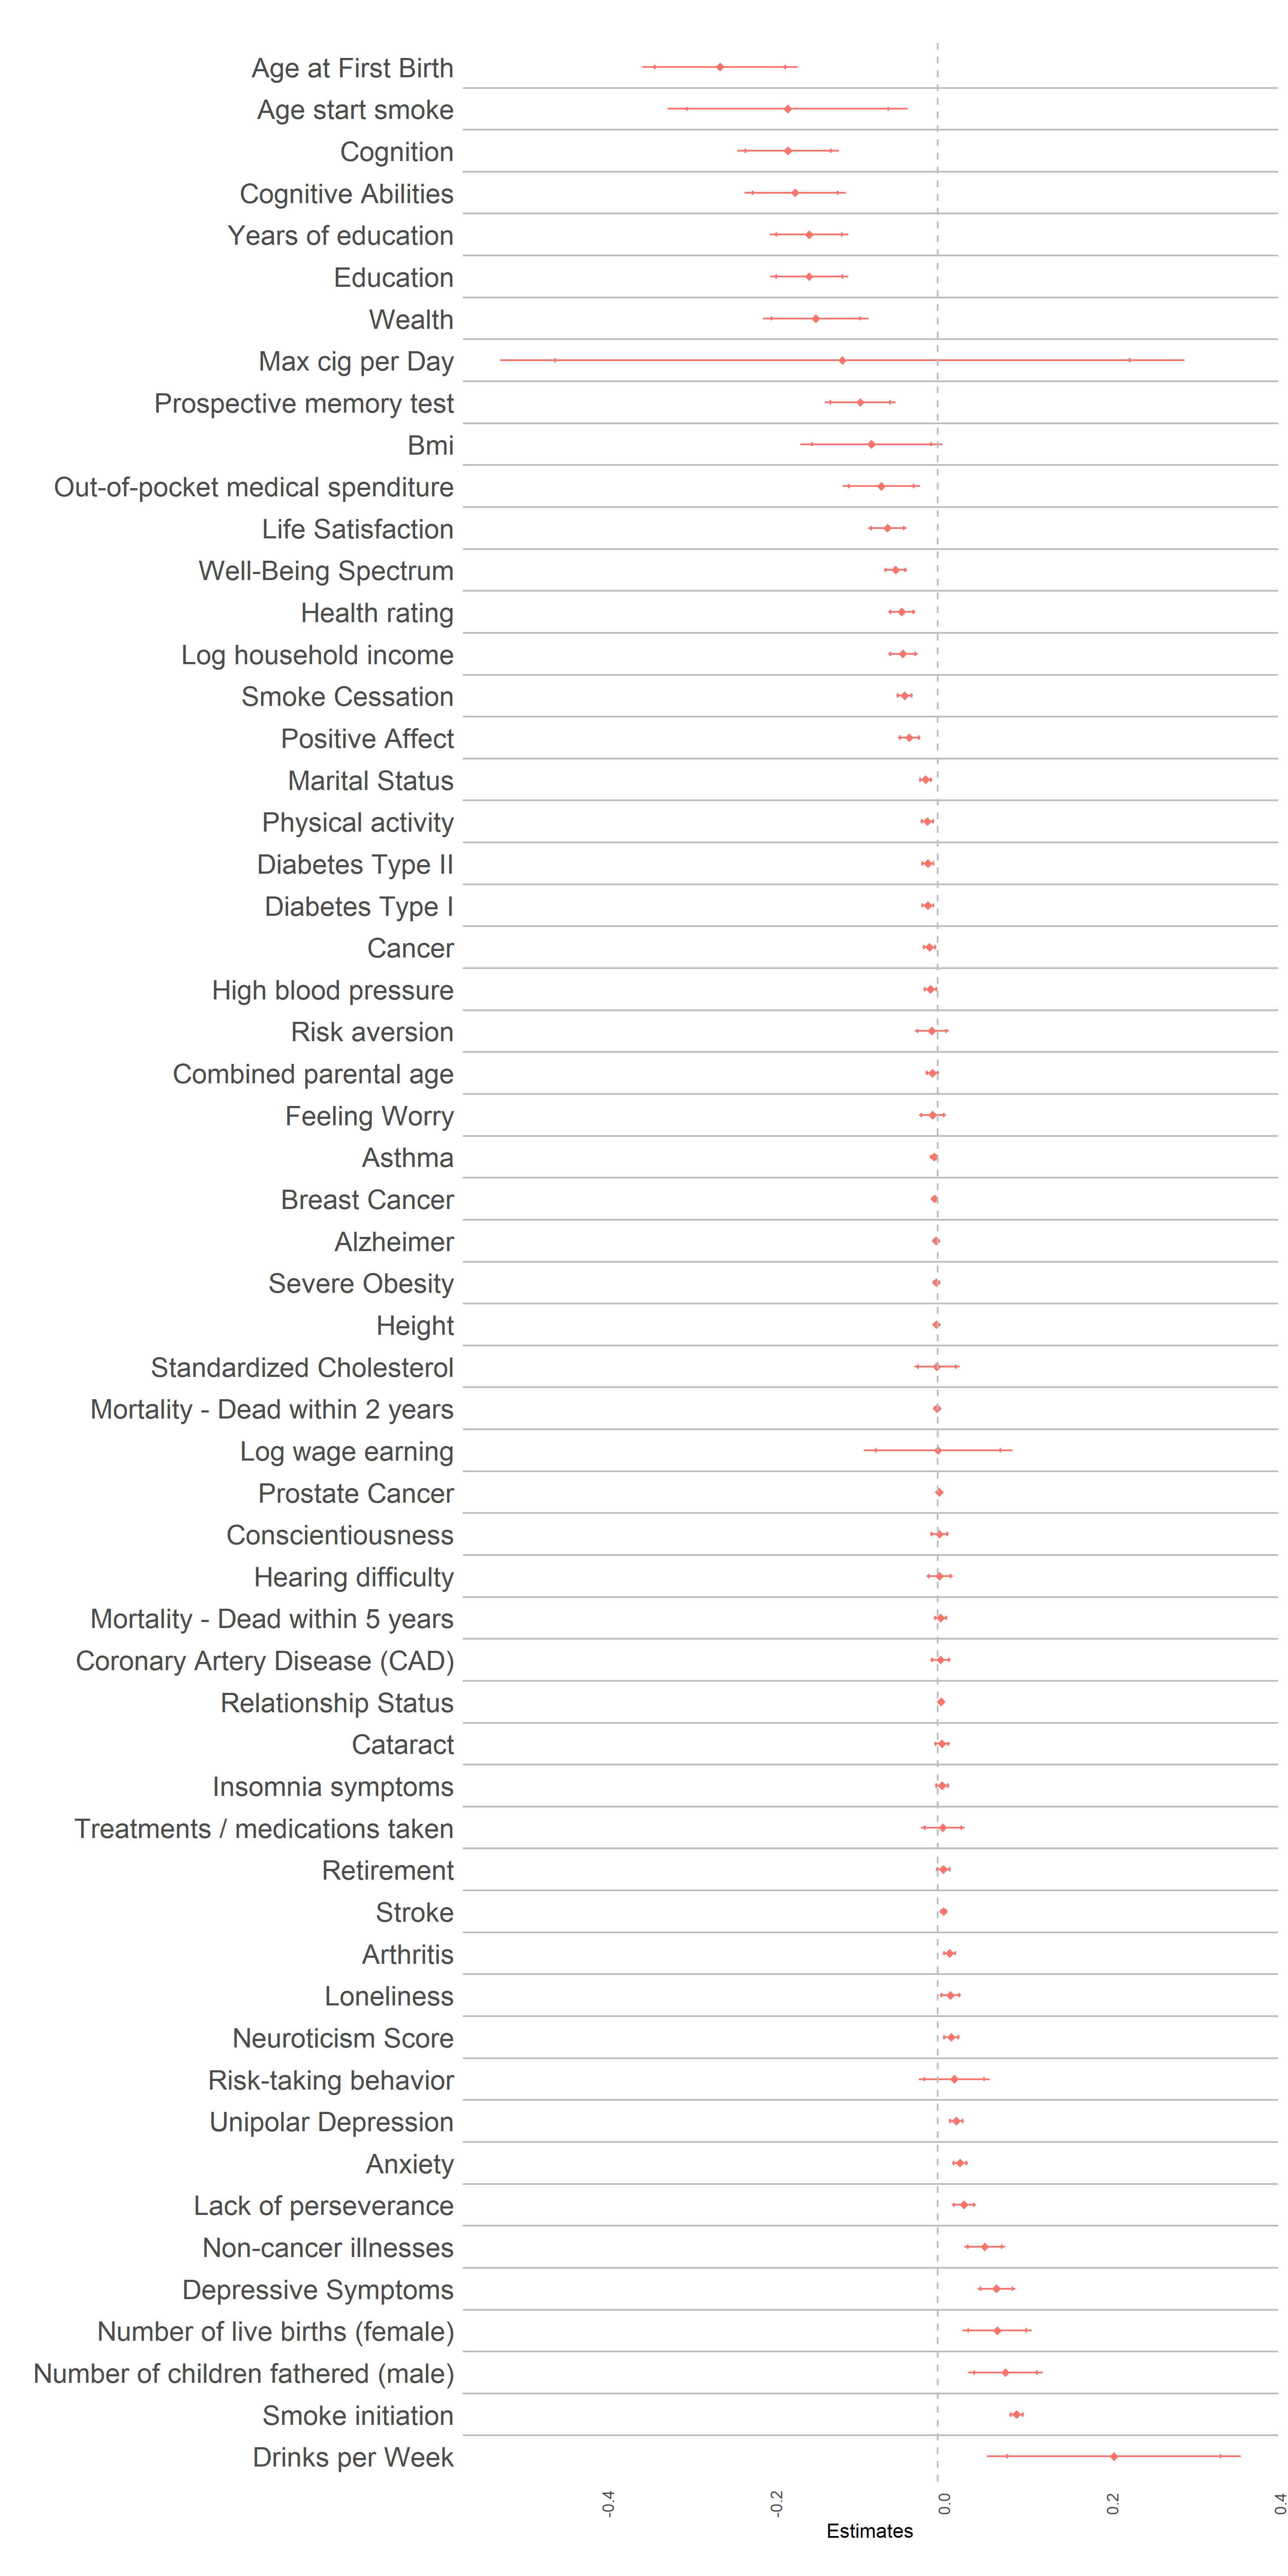
\includegraphics[height=0.7\textheight]{../3_output/make_histograms/PGSprediction.png}
	\caption{PGS distribution and correlation with smoking behavior.
	\label{fig:PGS_pred}}
	\vspace{-0.8cm}
	\floatfoot{
	\textit{Notes:} Plot of estimated coefficients associated with the PGS (entered linearly) from several OLS regressions of the different outcomes displayed on the y-axis on the PGS, age, age squared, age cubed, sex, and the first 10 principal components of the genomewide matrix.
	\\ \textit{Data used}: HRS waves 1-13, restricted to observations with age between 60 and 70 years.
	}
	\end{center}
\end{figure}

As shown in Figure \ref{fig:PGS_gender_cv}, the PGS is mildly correlated with gender and almost uncorrelated with the probability of suffering from a health shock.

\begin{figure}[ht]
	\begin{center}
		\subfigure[\textsf{PGS distribution and correlation with female gender.}]{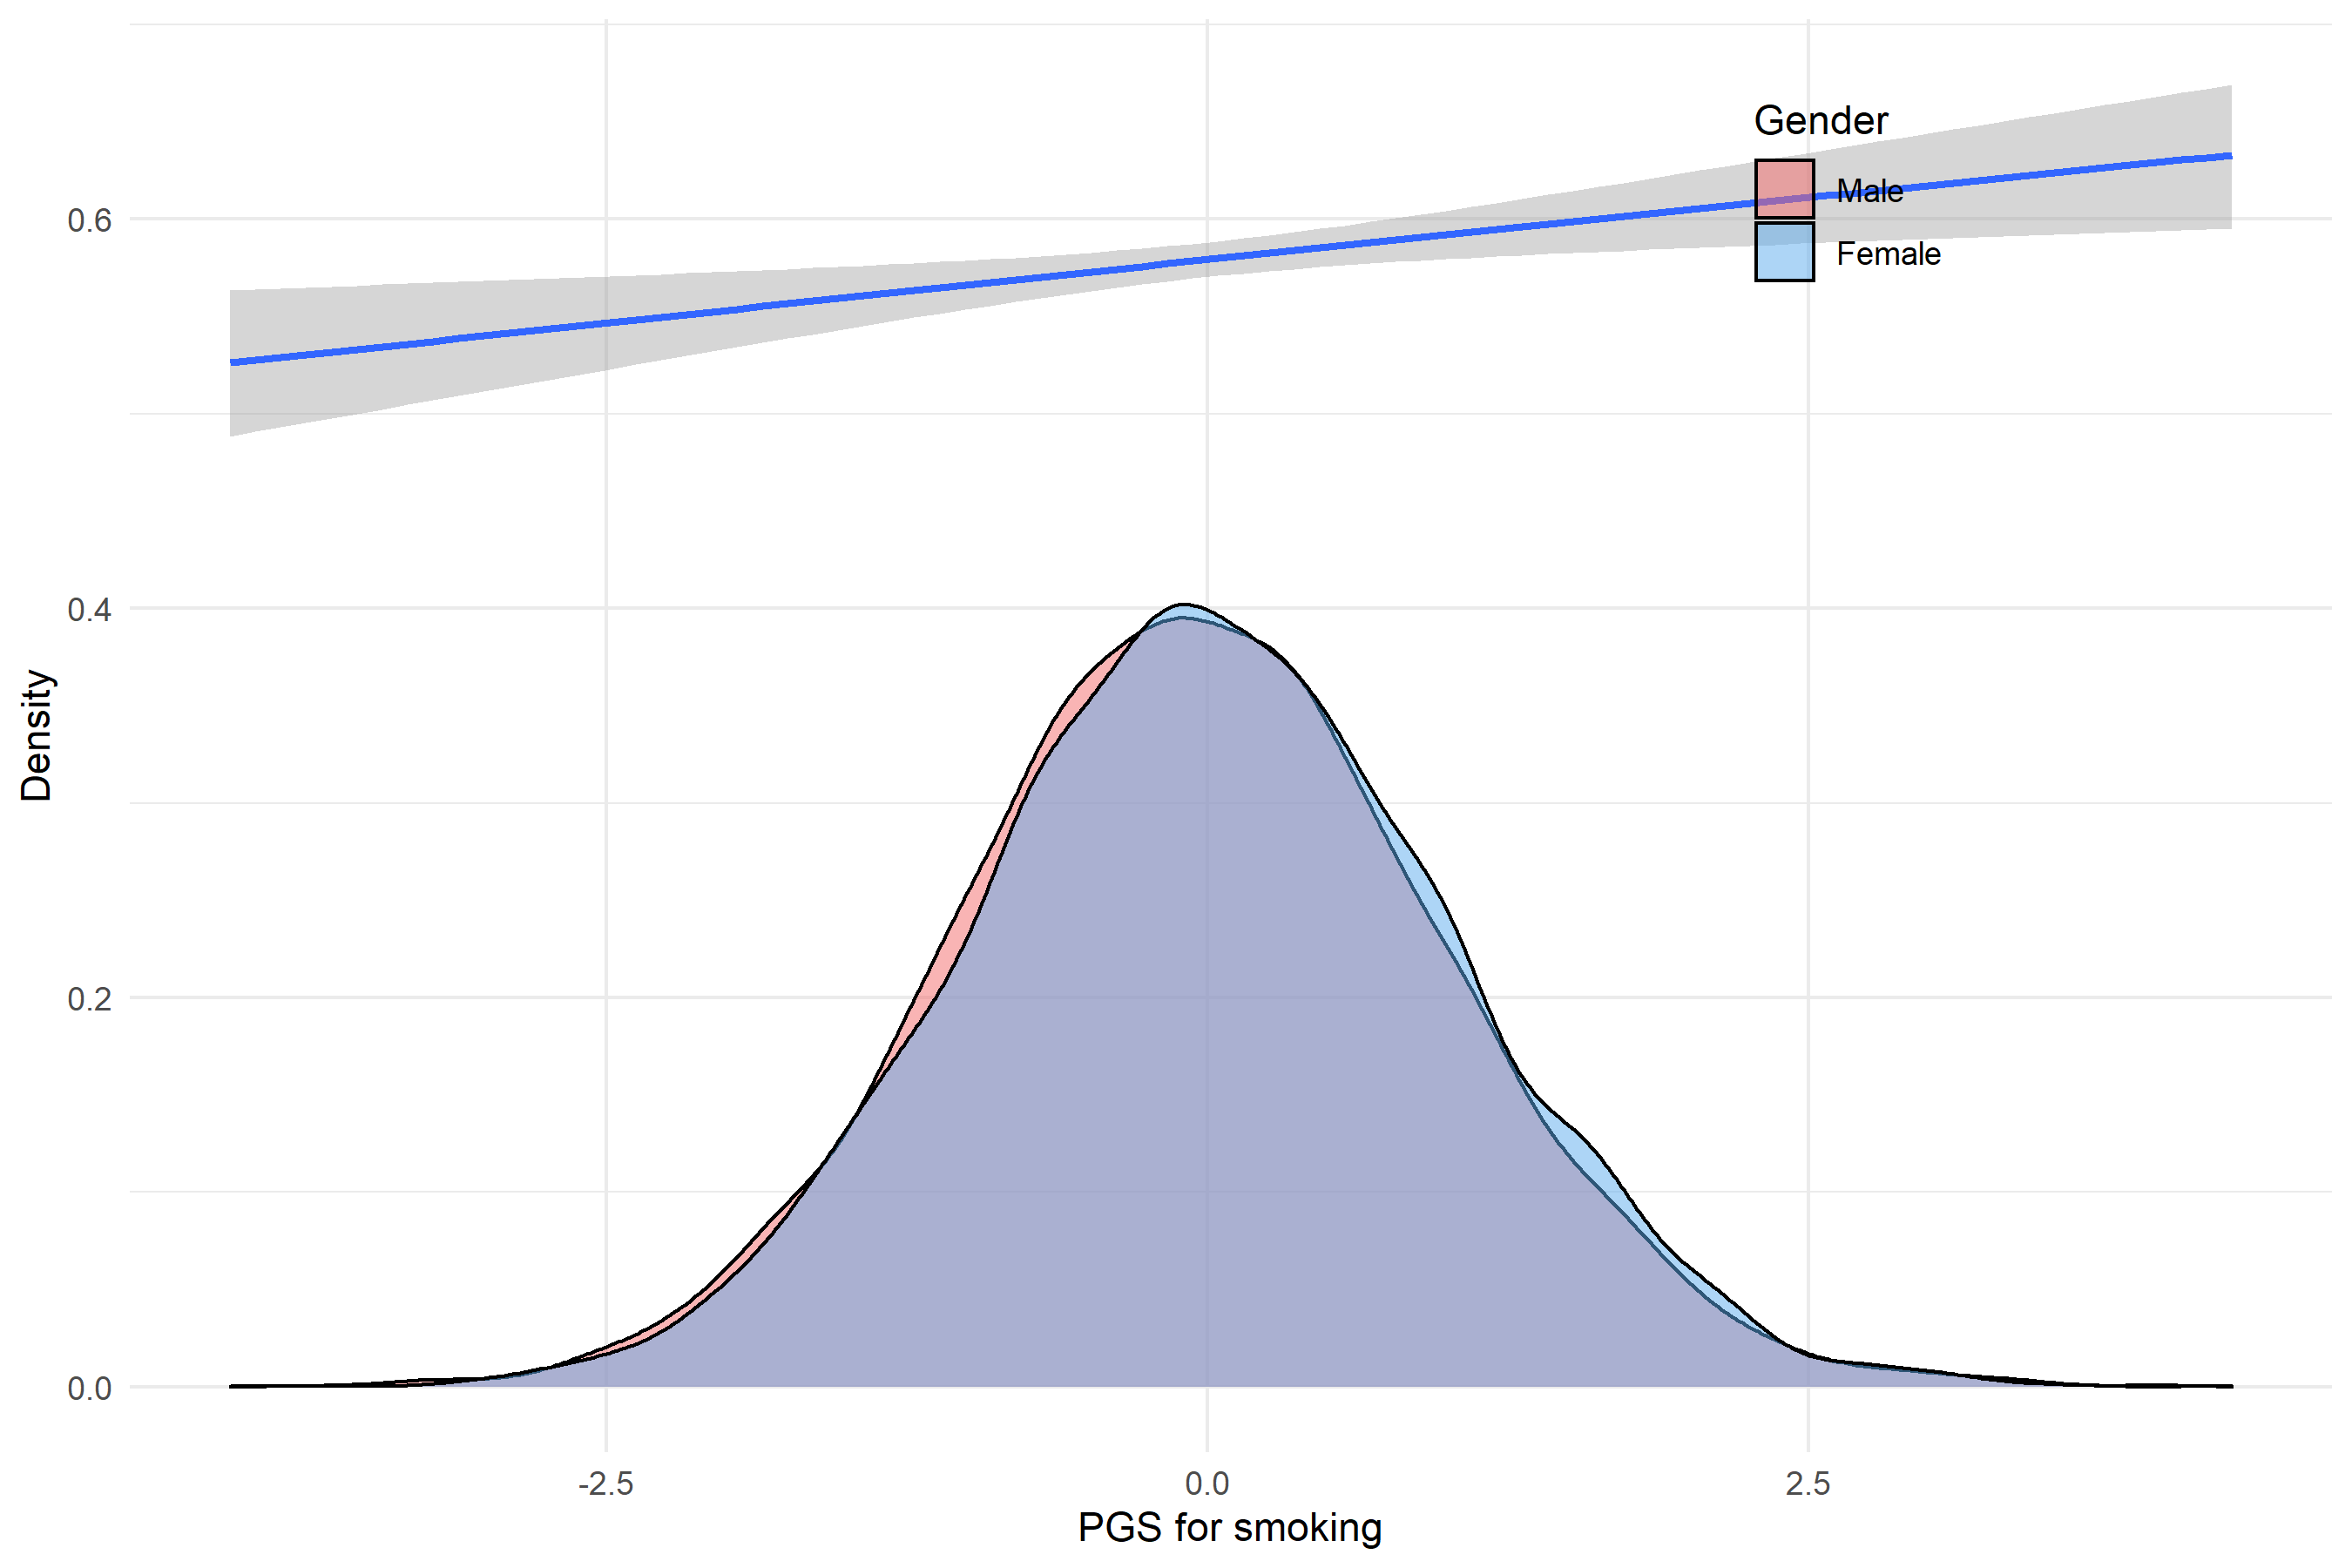
\includegraphics[width=8cm]{../3_output/make_histograms/pgs_density_6070_female_smooth.png}}
		\subfigure[\textsf{PGS distribution and correlation with the health shock.}]{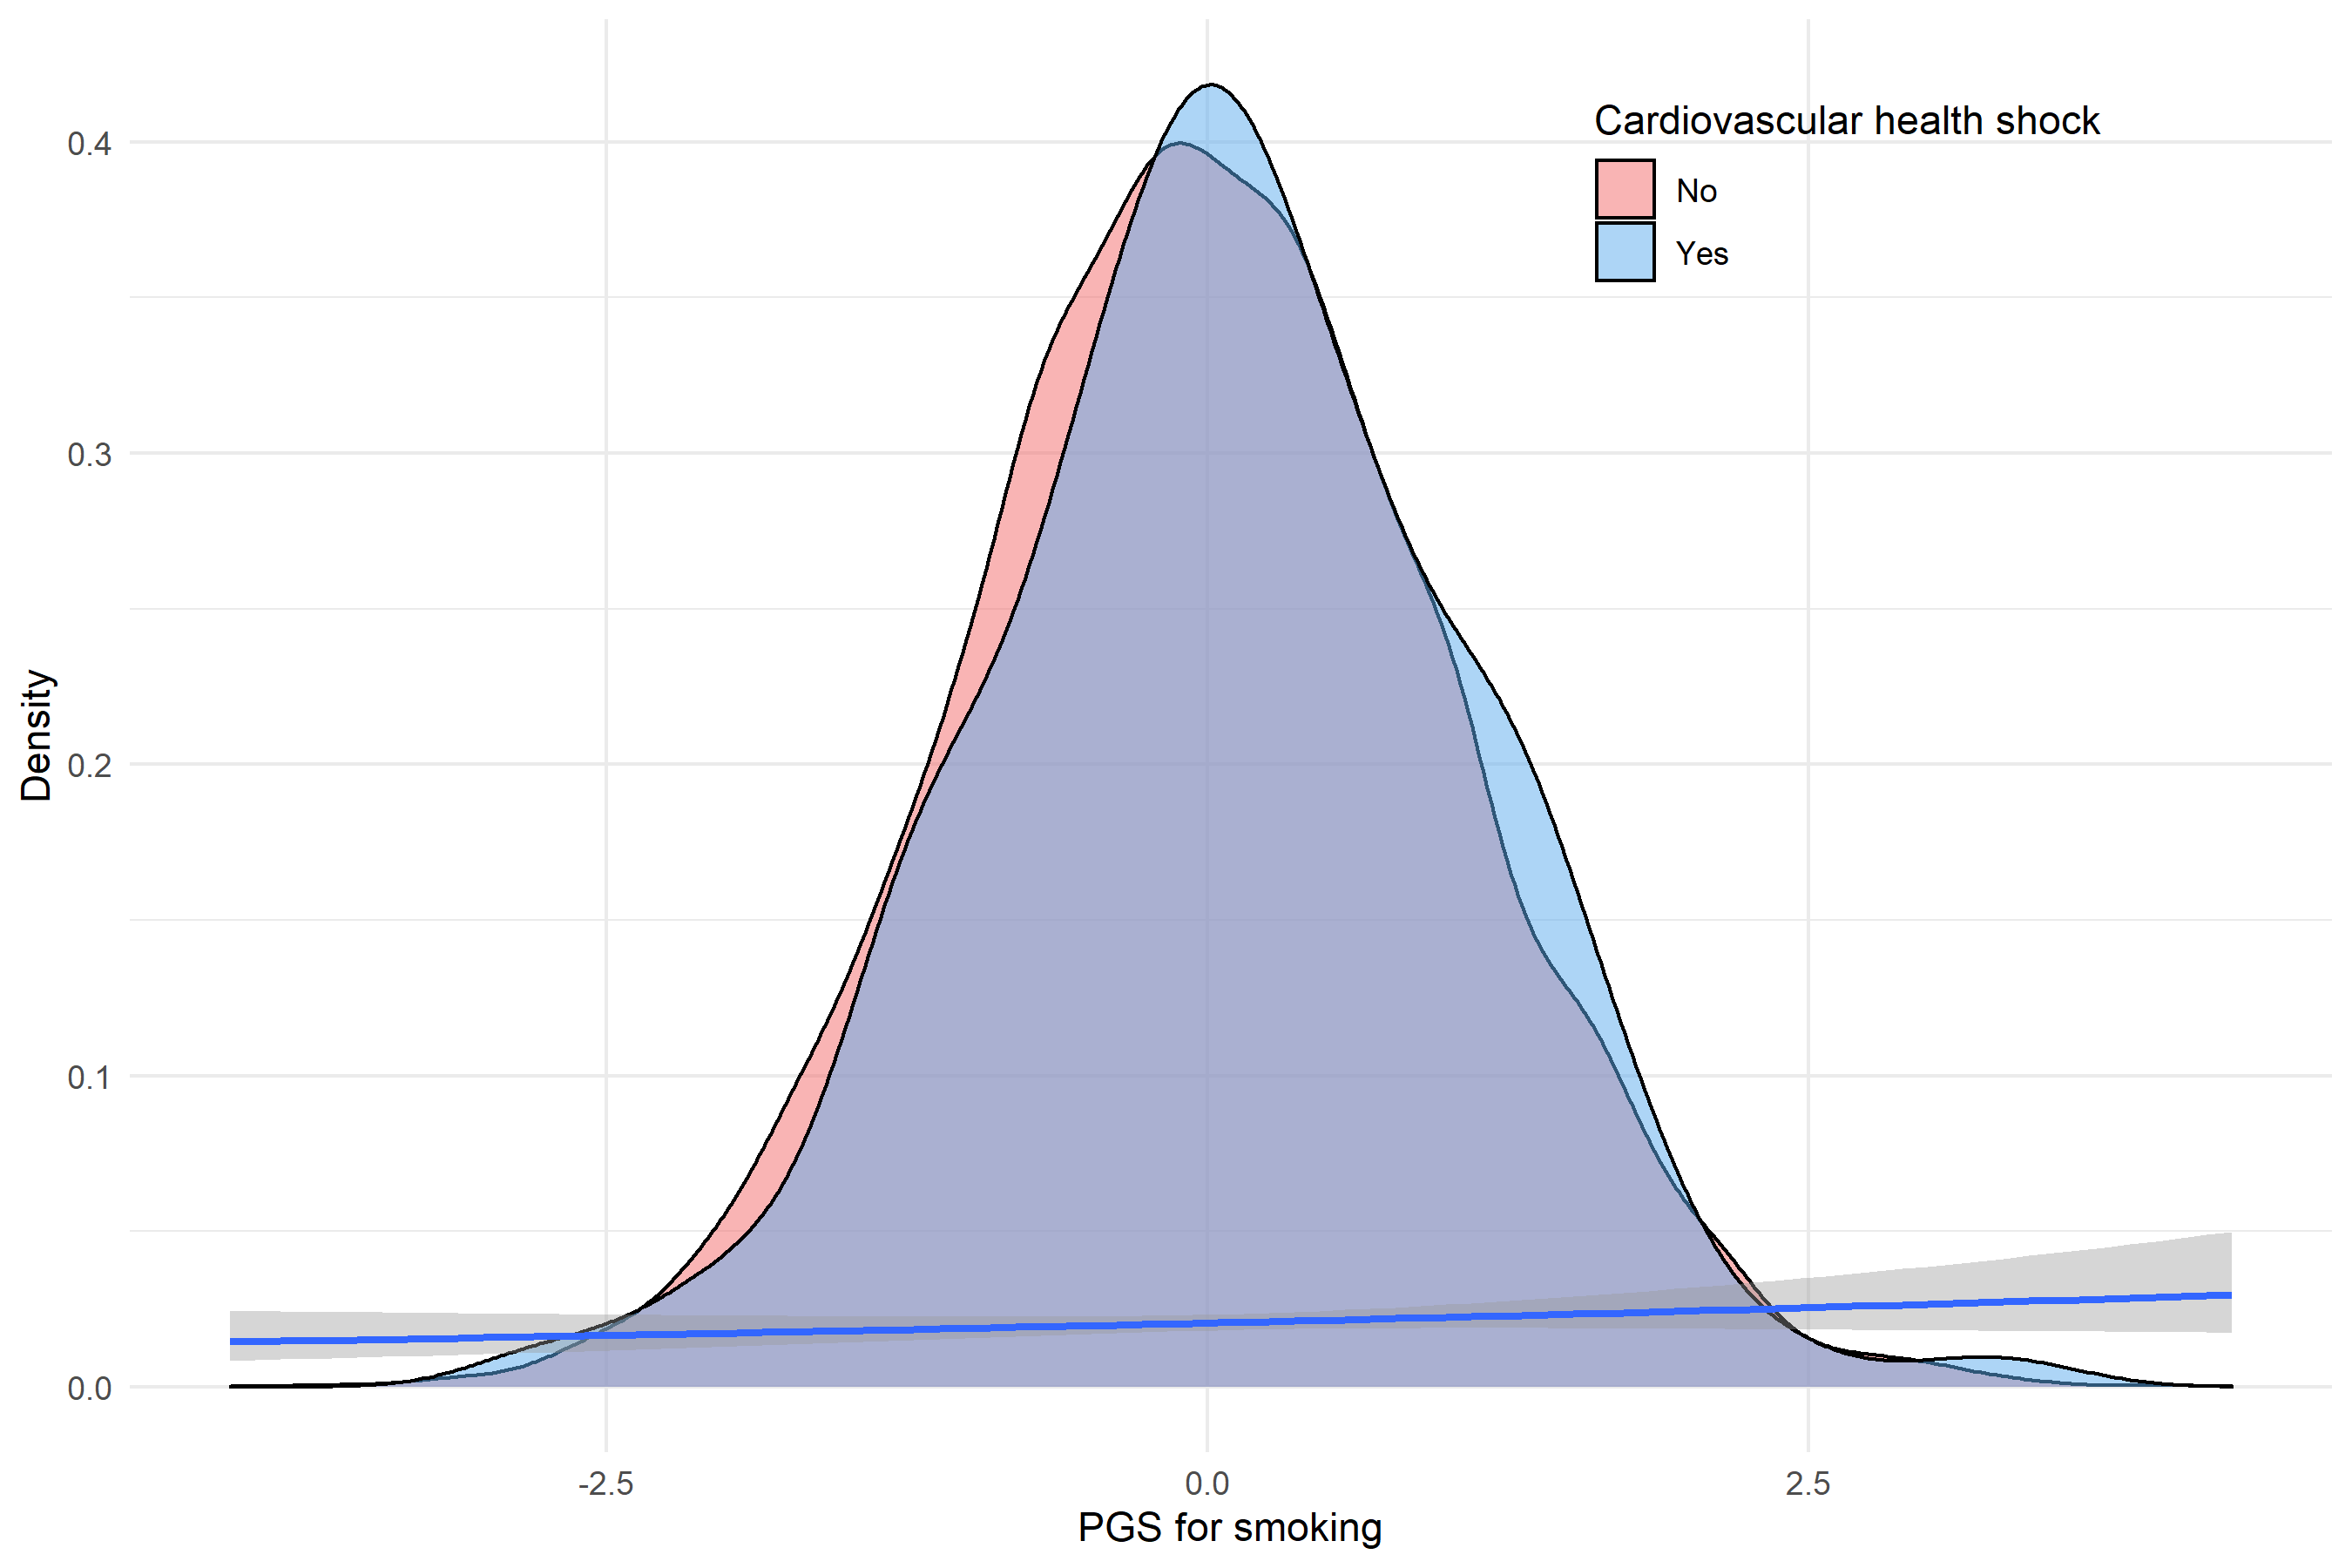
\includegraphics[width=8cm]{../3_output/make_histograms/pgs_density_6070_cv_smooth.png} }
		\caption{PGS for Regular Smoking and Smoking Behavior in the HRS Data
			\label{fig:PGS_gender_cv}}
	\vspace{-3ex}
	\floatfoot{
	\textit{Notes:} Distribution of Polygenic Score (PGS) for baseline smokers (blue) and non-smokers (red).
	Generalized linear smoothed correlation between current smoking and PGS shown in the blue line (with 95\% confidence intervals in shaded grey area).
	\\ \textit{Data used}: HRS waves 1-13, restricted to observations with age between 60 and 70 years.
	}
	\end{center}
\end{figure}


%Figure \ref{fig:PGS} shows how this binary indicator for genetic risk for smoking as well as the original PGS relate to reported smoking behavior in the HRS data (considering all respondents aged between 60 and 70, without excluding baseline never-smokers).
%Panel (a) of Figure \ref{fig:PGS} shows a clear level difference in the fraction of smokers between the high- and low-PGS groups. The age pattern of smoking was very similar across the 2 groups. Panel (b) of Figure \ref{fig:PGS} shows the distribution of the PGSs for those who were smokers at baseline and for those who were not. By visual inspection, the distribution of scores is centered around a higher level for baseline smokers than it is for baseline non-smokers.
%
%\captionsetup{format=cancaption,labelformat=cancaptionlabelC, width = \textwidth}
%\begin{figure}[ht]
%	\begin{center}
%		\subfigure[\textsf{Mean Smoking Status by Age, Stratified by Genetic Group}]{\includegraphics[width=8cm]{../3_output/smk_over_time/graph_6070plot_agebypgs.png}  }
%		\subfigure[\textsf{Distribution of PGSs, Stratified by Baseline Smoking Status}]{\includegraphics[width=8cm]{../3_output/make_histograms/graph_6070smoken.png} }
%		\caption{PGS for Regular Smoking and Smoking Behavior in the HRS Data
%			\label{fig:PGS}}
%		\floatfoot{\vspace{-3cm} \\
%			\textsf{Low PGS = lowest tertile of the polygenic score distribution; high PGS = upper two tertiles of the polygenic score distribution.\\
%				\textit{Data used}: HRS waves 1-12, restricted to observations with age between 60 and 70 years.}}
%	\end{center}
%\end{figure}

\vspace{2mm}

\subsection{Statistical Analysis}

\subsubsection{Age Pattern of Health Shock Incidence}
\label{supsec:age_pattern_cv}
With the data used in this study, it was not possible to narrow down the exact timing of a health shock to more than the between-survey 2-year window. Therefore, the probability of having a health shock at a specific age could not be determined. What could be said from this data about the age at the health shock is that for all shocks reported at ages 64 or below, the shocks must have occurred before the age of 65. Similarly, for all health shocks reported at ages 67 or above, the shocks must have occurred after the age of 65. For shocks reported at interview ages 65 or 66, it could not be determined whether the shock occurred before or after age 65 (as interviews were conducted biennially). \\

Figure \ref{fig:cv_prob} visualizes the fraction of HRS respondents who reported experiencing a health shock since the last survey wave at a given interview age, stratified both by genetic group and by gender. By visual inspection, there seems to be a positive trend in the fraction of respondents reporting health events with age, with frequent deviations but no obvious jump between 64 and 67. \\


\begin{figure}[!tbp]
	\begin{center}
		\caption{Percentage of Reported Health Shocks by Age \label{fig:cv_prob}}
		\subfigure[\textsf{Cutoff at age 64}]{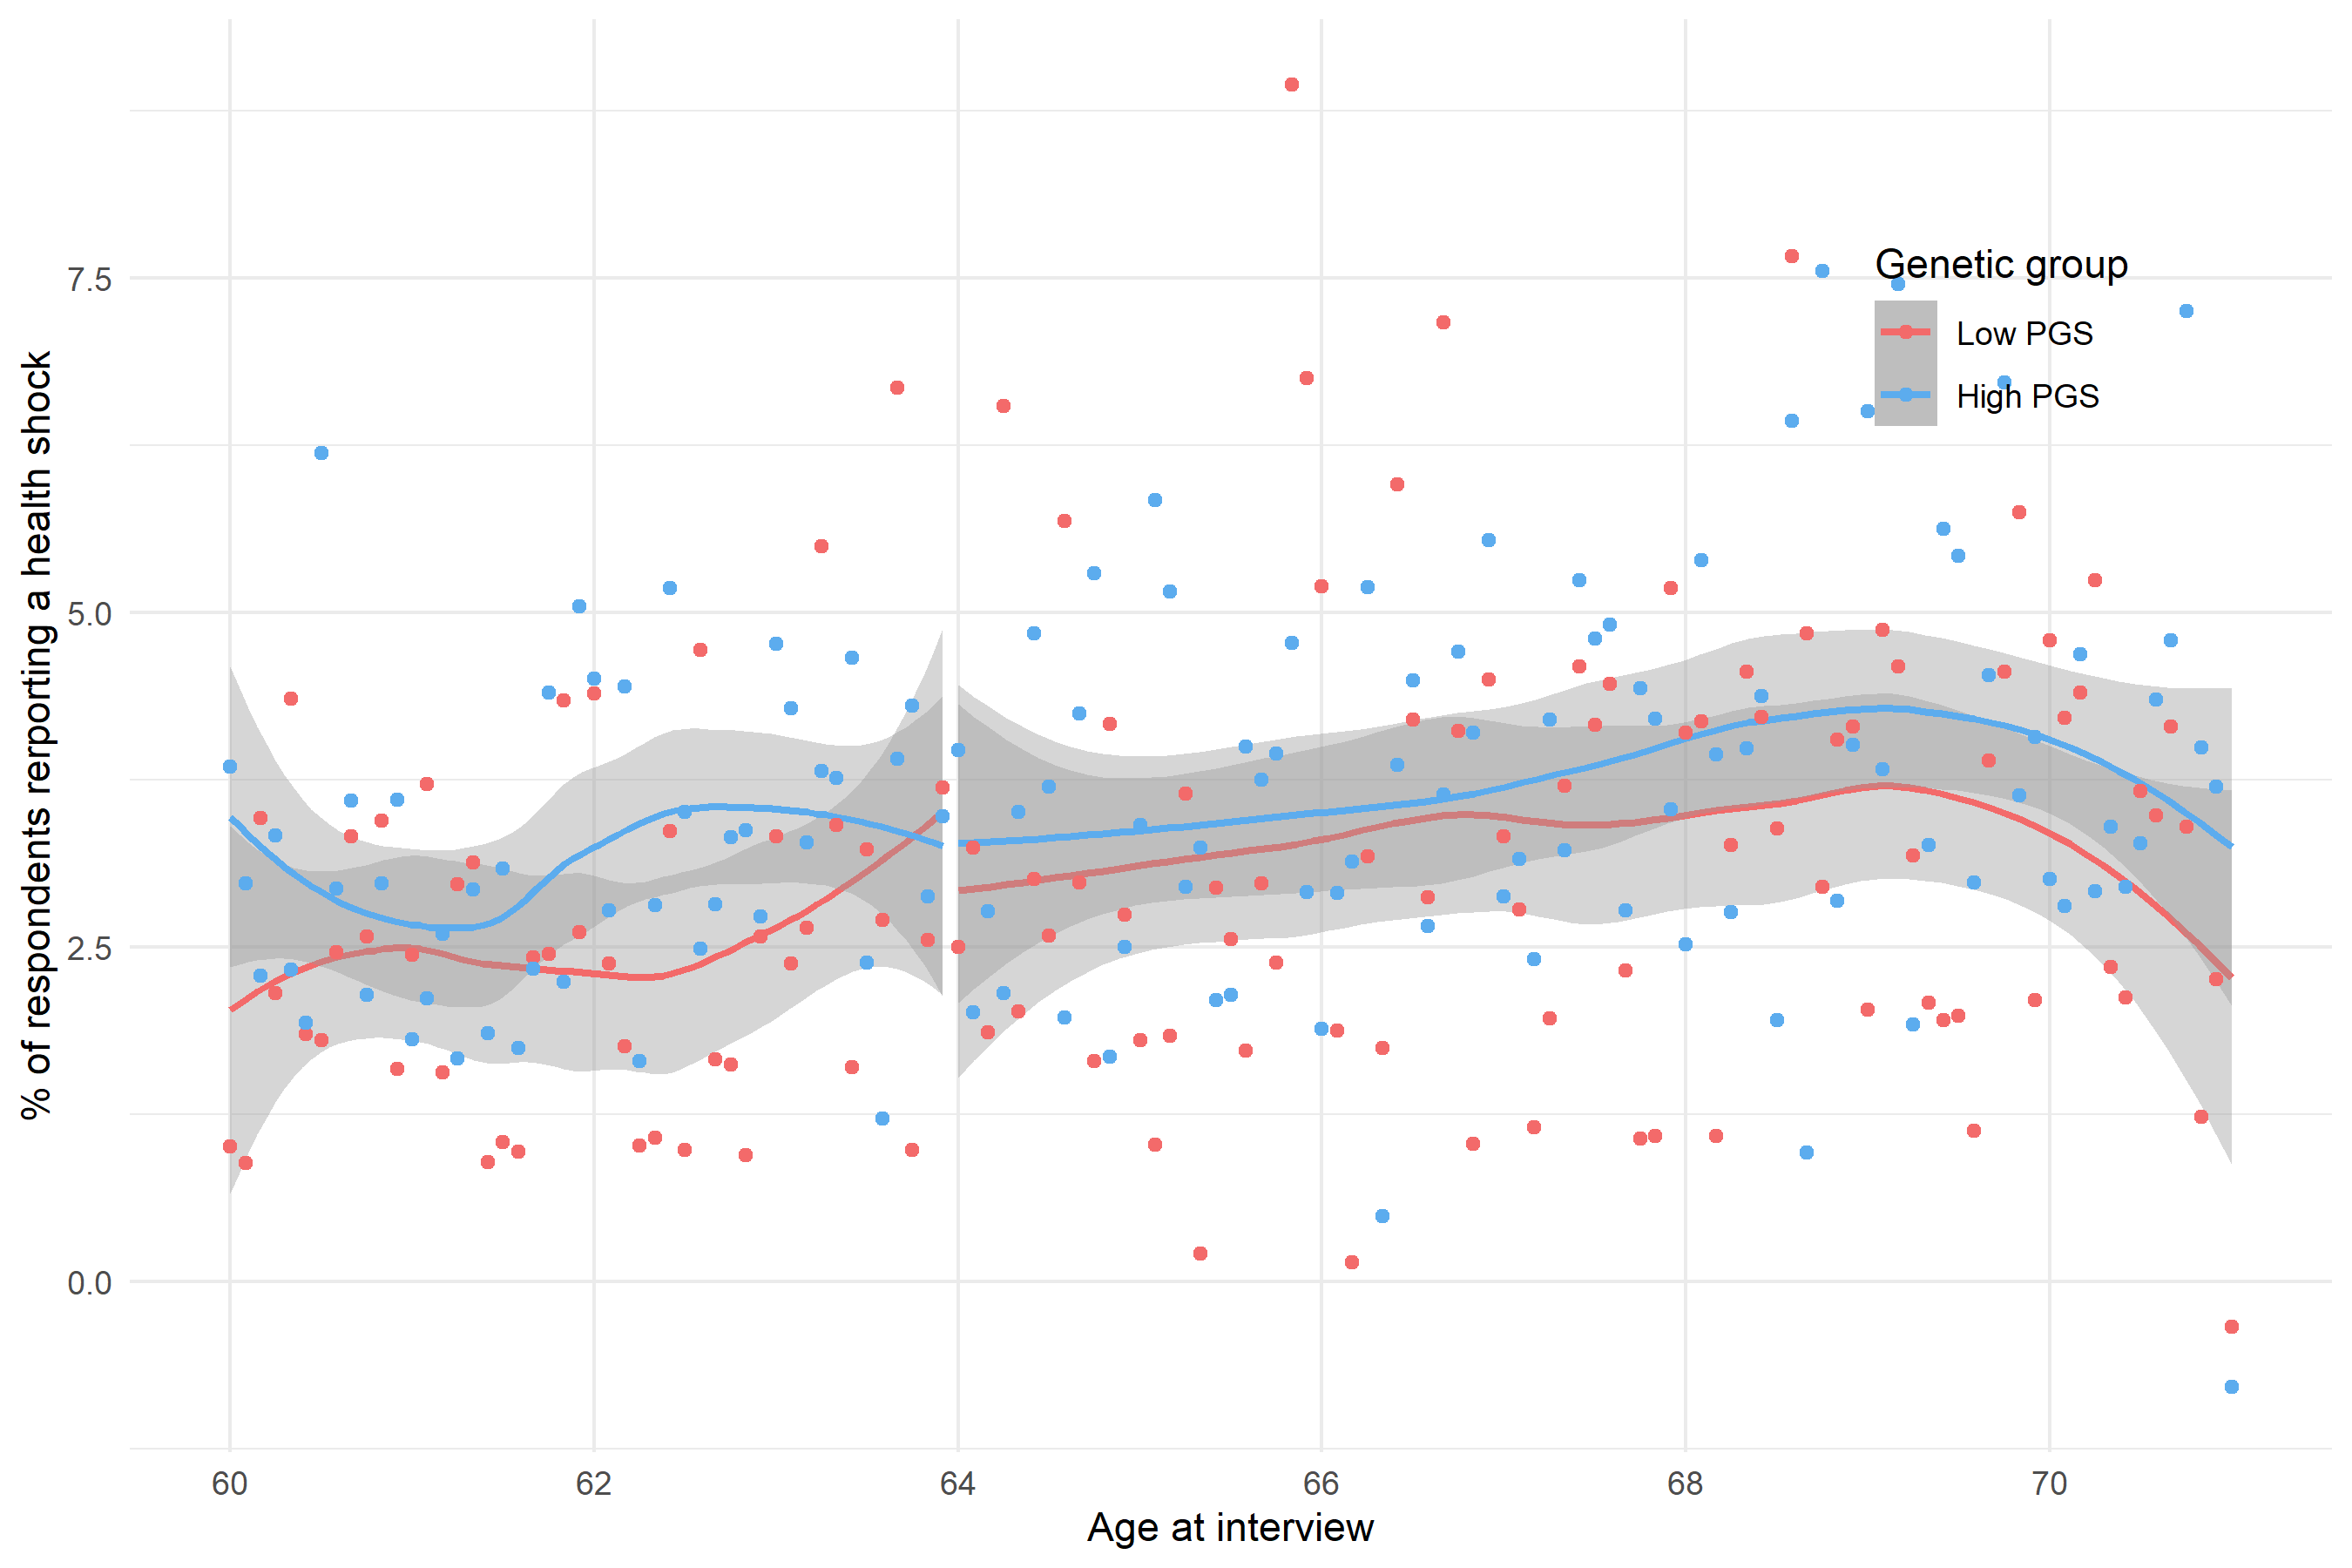
\includegraphics[width=5cm]{../3_output/over_time/graph_6070_cut64cvrdd_agebypgs.png}}
		\hfill
		\subfigure[\textsf{Cutoff at age 65}]{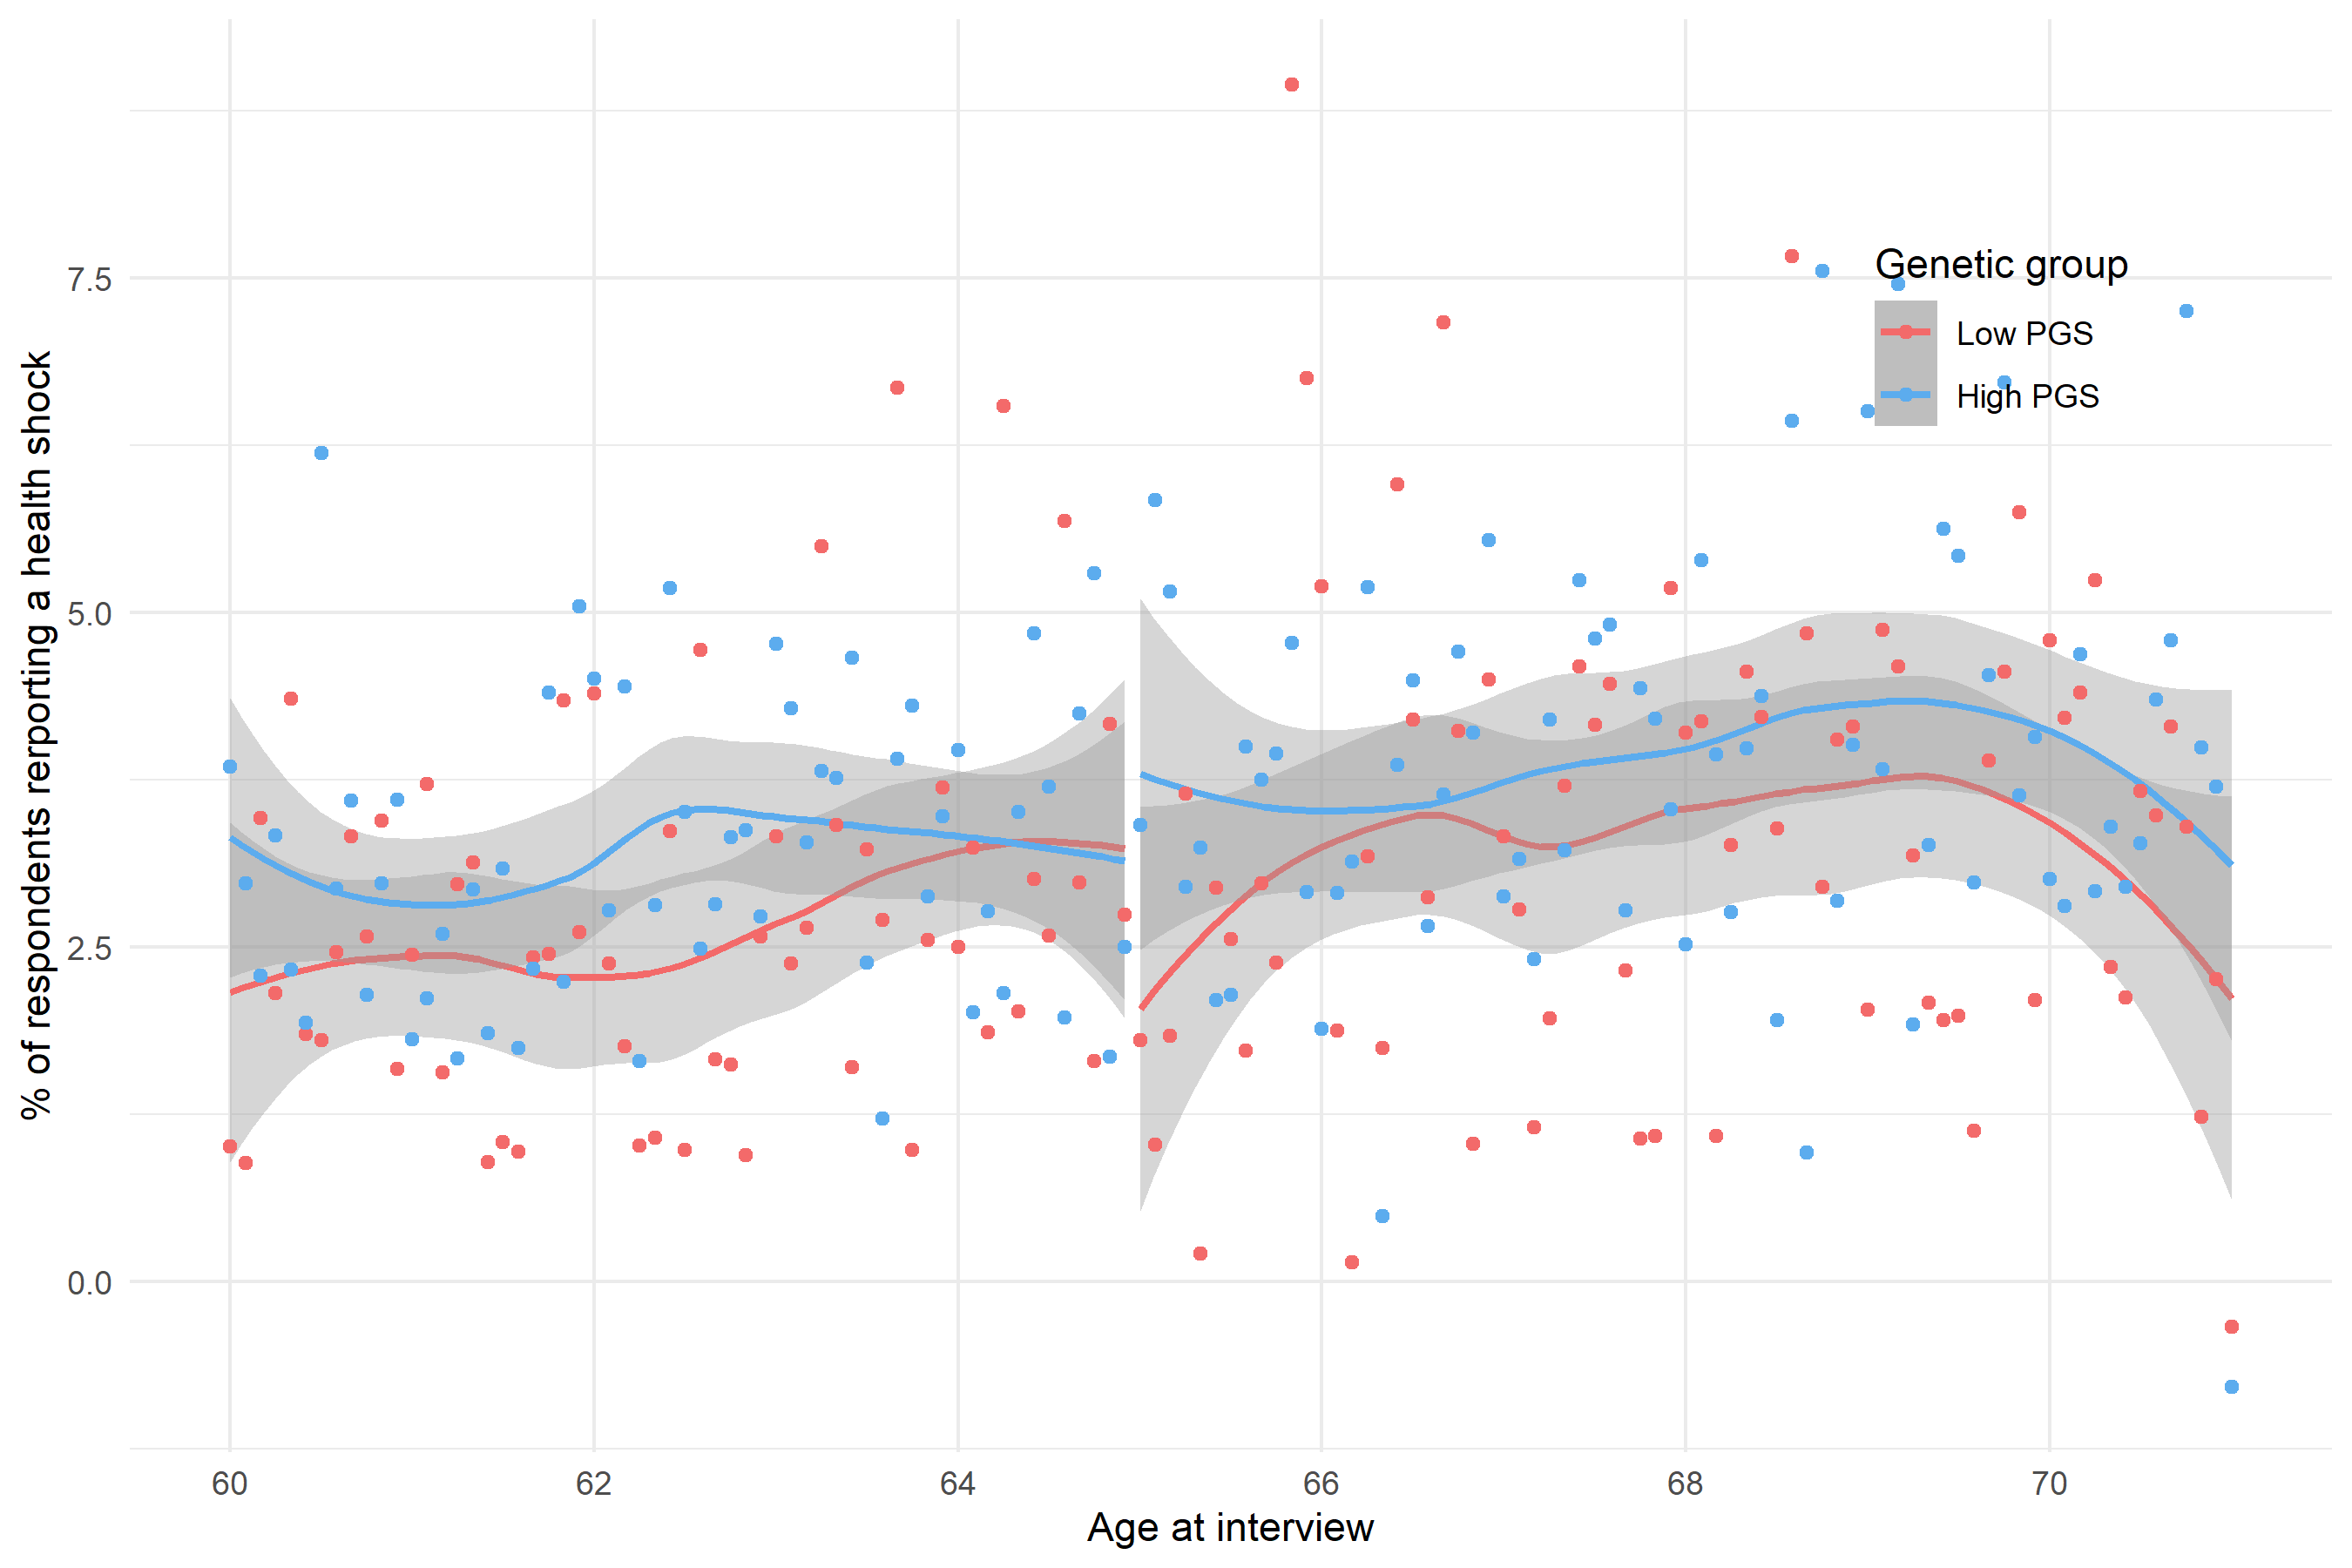
\includegraphics[width=5cm]{../3_output/over_time/graph_6070cvrdd_agebypgs.png}}
		\hfill
		\subfigure[\textsf{Cutoff at age 66}]{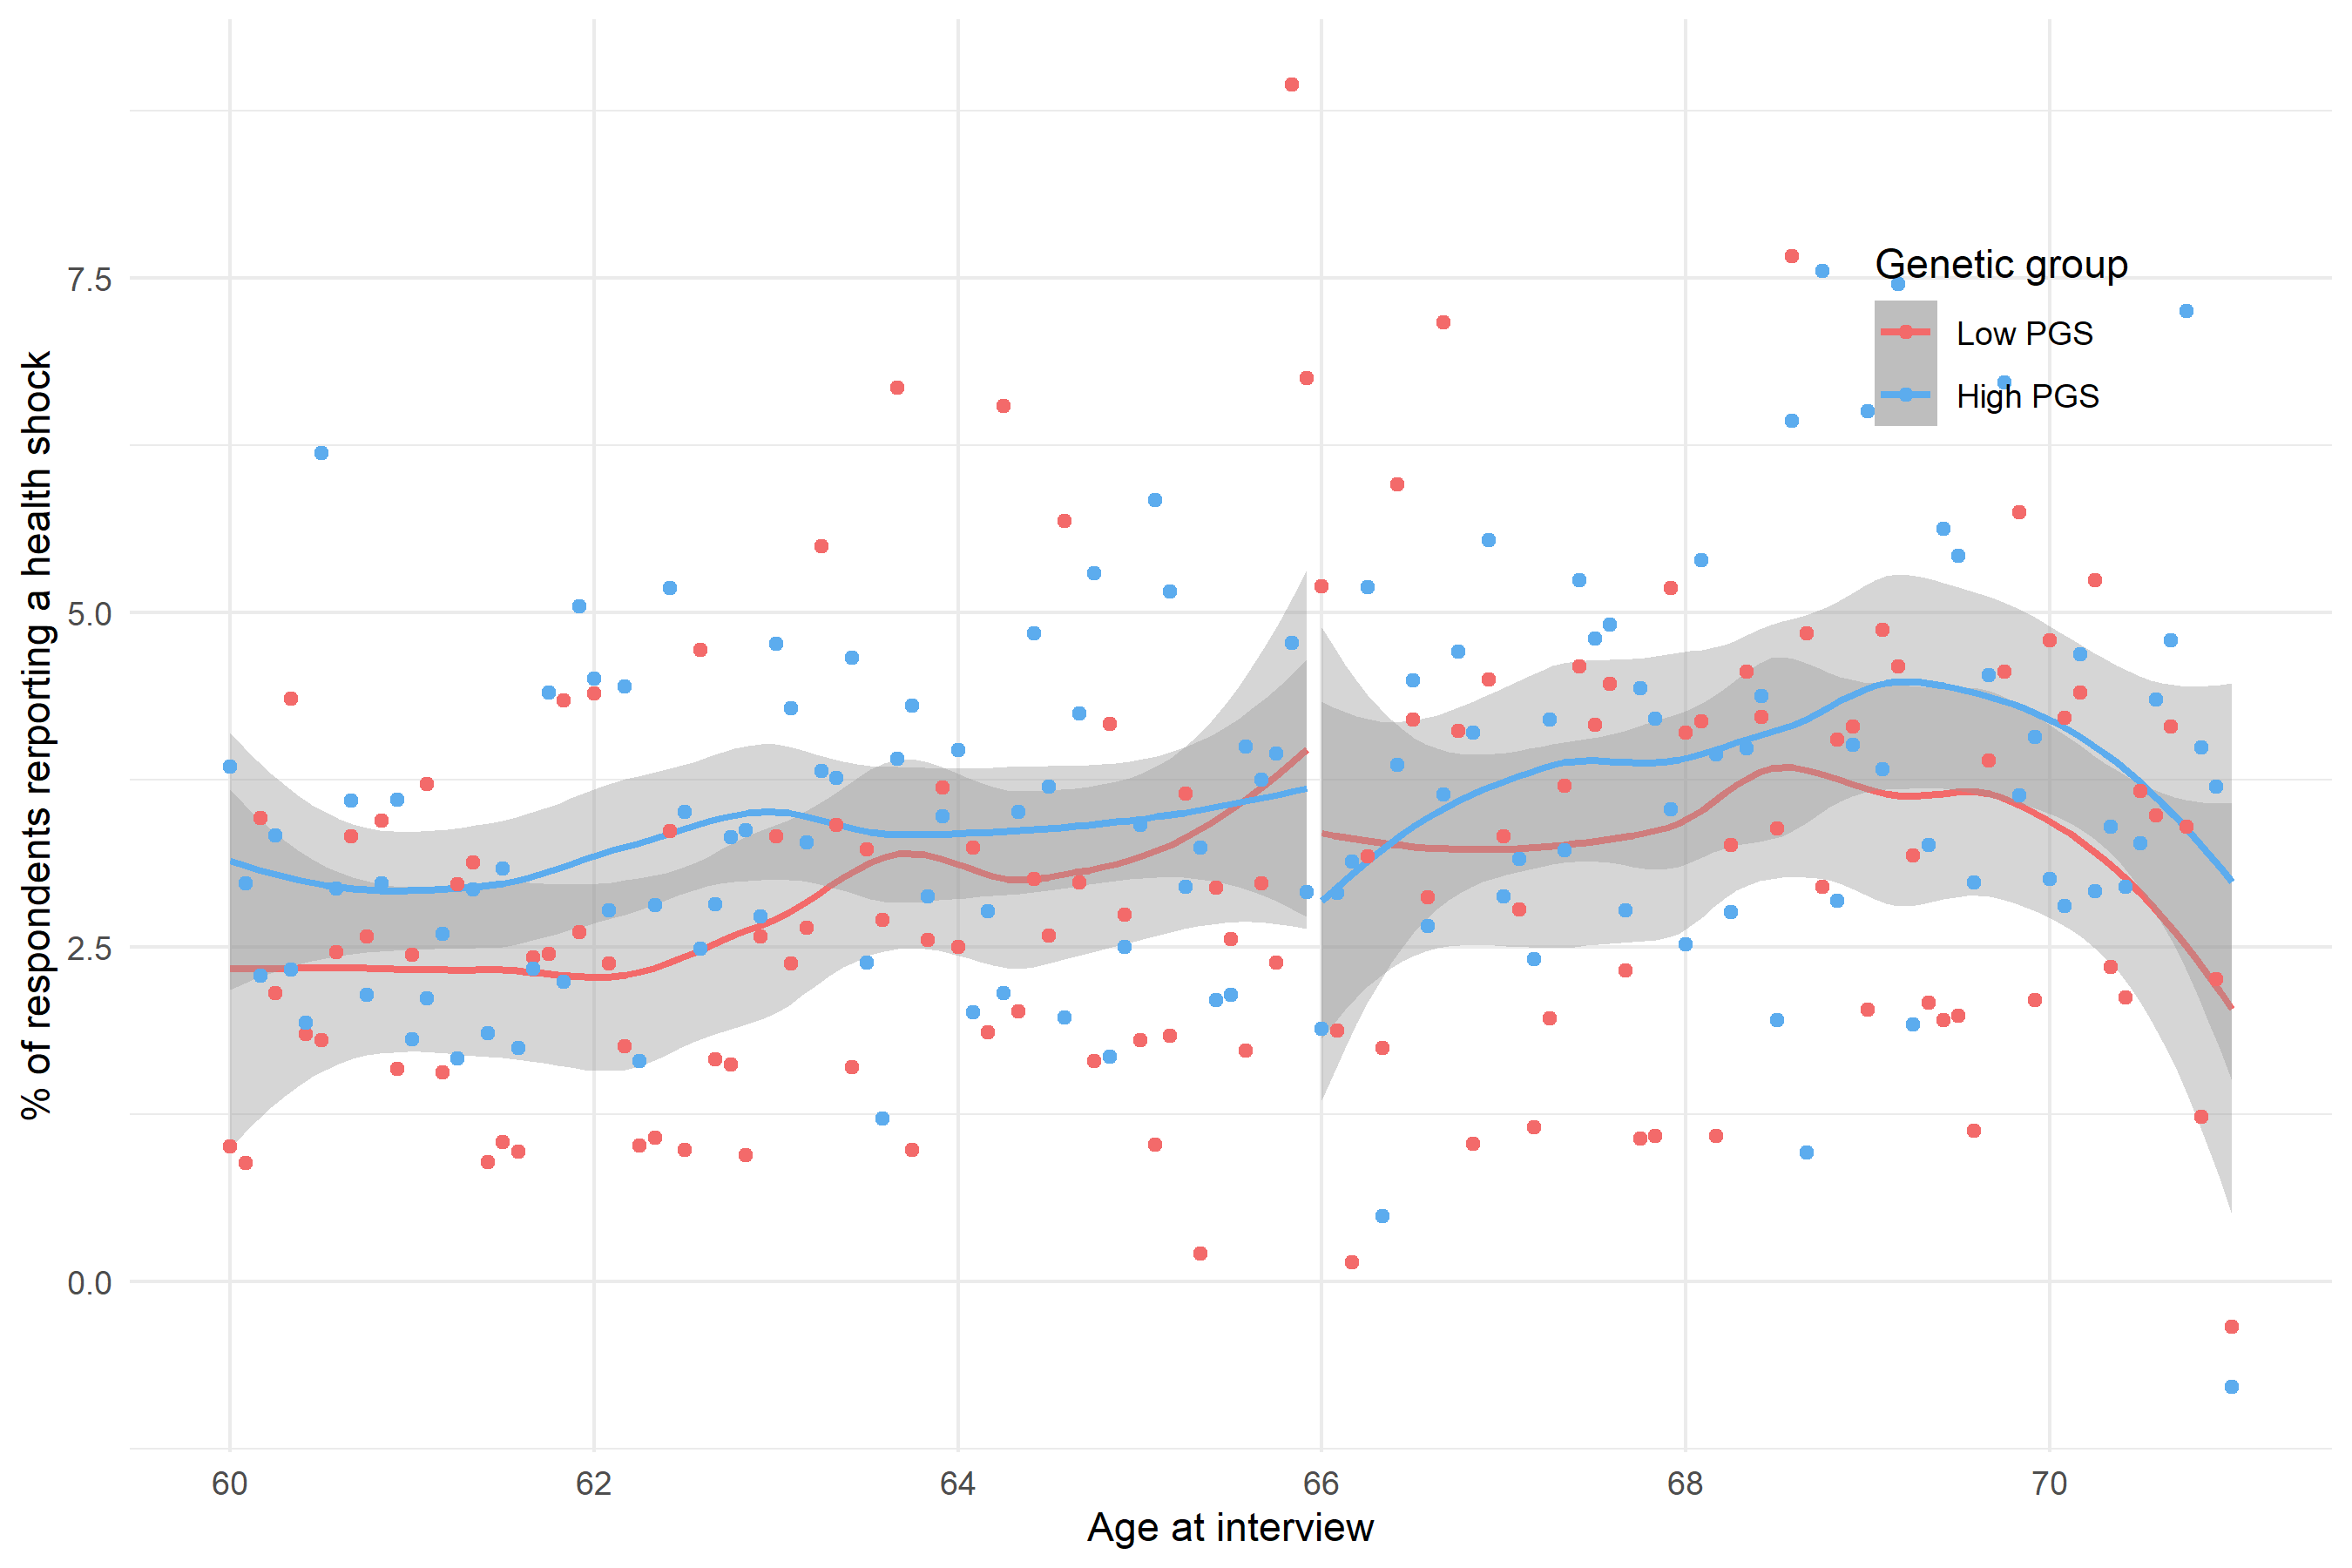
\includegraphics[width=5cm]{../3_output/over_time/graph_6070_cut66cvrdd_agebypgs.png}}
		\floatfoot{ \vspace{-0.8cm} \\
		Self-reported indicator of having been diagnosed for the first time with a cardiovascular condition since the last HRS survey.
		Age refers to the time of the survey, not the time of the health shock, which is unknown up to a 2-year windows, since HRS surveys are bi annual.
		Bin-scattered plot and generalized linear smoothed correlation between age at interview and cardiovascular health shock shown in red (low PGS) and blue (high PGS).
		Linear smoothed correlation estimated separately to the left and to the right of age cutoff: (a) age 64; (b) age 65; (c) age 66. \\
		\textit{Data used}: HRS waves 1-13, restricted to observations with age between 60 and 70 years.
		}
	\end{center}
\end{figure}


To formally test for a jump or change in trend in the incidence of health shocks around the age of 65, a segmented regression approach was used. Specifically, we tested if the change between the percentage of respondents who reported a health shock at age 64 and the percentage of respondents who reported a health shock at age 67 was larger than what could be explained by a linear age trend. For this test, all observations where respondents were aged 65 or 66 were excluded. For all remaining observations, the binary health shock indicator ($shock$) was regressed on the age variable ($age$), a post-age-67 indicator variable ($post67$), and a post-age-67 trend ($post67slope$):
\begin{align} \label{supcv_regression}
shock_{it} \thinspace = \thinspace \beta_0 + \beta_1 \thinspace age_{it} + \beta_2 \thinspace post67_{it} + \beta_3 \thinspace post67slope_{it} + \varepsilon_{it}
\end{align}

The post-age-67 indicator variable was defined to take the value 1 if a respondent was aged 67 or older at the time of the HRS interview. Therefore, it guaranteed that any potential health shocks were experienced after the age of 65. The post-age-67 slope variable was a continuous variable coded 0 up to and including age 67, and increased sequentially from 1 thereafter. $\beta_1$ captured the general age trend in the probability of reporting a health shock; $\beta_2$ estimated the jump in the report of health shocks at age 67; $\beta_3$ reflected changes in the age trend of reported health shocks after age 67.\\


The linear probability model in Equation (\ref{supcv_regression}) was estimated using ordinary least squares (OLS) regression for (i) the study sample (HRS waves 1-12, restricted to observations with age between 60 and 70 years, and additionally excluding all observations with ages 65 or 66), (ii) both genetic groups separately, and (iii) both men and women separately. Estimation results are shown in Table \ref{suptab:cv_regression}. Across all groups, there were no statistically significant jumps for health shocks reported at age 67 compared to age 64 (accounting for a linear age trend). Similarly, the age trend was not significantly different after age 67 than before. In the study sample and in the low-PGS group, the increase with age in the probability of reporting a health shock was statistically significant.


%%%%%%%%%%%%%%%%%%%% PROBABILITY OF A CV SHOCK REGRESSION %%%%%%%%%%%%%%%%%%%%
\captionsetup{width = 11cm}
% Table created by stargazer v.5.2 by Marek Hlavac, Harvard University. E-mail: hlavac at fas.harvard.edu
% Date and time: Fr, Apr 27, 2018 - 15:00:48
\begin{table}[ht] \centering
	\caption{Coefficients from Estimating the Linear Probability Model in Equation (\ref{supcv_regression}) Using OLS}
	\label{suptab:cv_regression}
	
% Table created by stargazer v.5.2.2 by Marek Hlavac, Harvard University. E-mail: hlavac at fas.harvard.edu
% Date and time: Thu, Mar 11, 2021 - 7:28:02 PM
\begin{tabular}{@{\extracolsep{5pt}}lccccc} 
\\[-1.8ex]\hline 
\hline \\[-1.8ex] 
 & \multicolumn{5}{c}{\textit{Dependent variable:}} \\ 
\cline{2-6} 
\\[-1.8ex] & \multicolumn{5}{c}{Probability of shock} \\ 
 & All & Low PGS & High PGS & Male & Female \\ 
\\[-1.8ex] & (1) & (2) & (3) & (4) & (5)\\ 
\hline \\[-1.8ex] 
 Age & 0.002$^{**}$ & 0.003$^{**}$ & 0.001 & 0.001 & 0.002$^{*}$ \\ 
  & (0.001) & (0.001) & (0.001) & (0.001) & (0.001) \\ 
  & & & & & \\ 
 Post-67 dummy & $-$0.001 & $-$0.008 & 0.002 & $-$0.002 & $-$0.0002 \\ 
  & (0.005) & (0.008) & (0.006) & (0.008) & (0.006) \\ 
  & & & & & \\ 
 Post-67 slope & $-$0.001 & $-$0.002 & 0.0003 & 0.001 & $-$0.002 \\ 
  & (0.001) & (0.002) & (0.002) & (0.002) & (0.002) \\ 
  & & & & & \\ 
 Constant & $-$0.072 & $-$0.156$^{*}$ & $-$0.031 & $-$0.057 & $-$0.081 \\ 
  & (0.049) & (0.083) & (0.061) & (0.080) & (0.062) \\ 
  & & & & & \\ 
\hline \\[-1.8ex] 
Observations & 39,062 & 13,035 & 26,027 & 16,476 & 22,586 \\ 
\hline 
\hline \\[-1.8ex] 
\textit{Note:}  & \multicolumn{5}{r}{$^{*}$p$<$0.1; $^{**}$p$<$0.05; $^{***}$p$<$0.01} \\ 
\end{tabular} 

		\begin{flushleft}
			Low PGS = lowest tertile of the polygenic score distribution; high PGS = upper two tertiles of the polygenic score distribution.\\
			 \textit{Data used}: HRS waves 1-13, restricted to observations with age between 60 and 70 years and non-missing smoking status, and additionally excluding all observations with ages 65 or 66.
			\vspace{5mm}
		\end{flushleft}
\end{table}
\captionsetup{width = \columnwidth}


\pagebreak

\subsection{Derivation of the effects from the OLS coefficients}
\label{appsec:derivation}
\subsubsection{OLS estimation: high and low PGS}
Current smoking status ($Y$) is regressed on the full set of interactions between the indicators for the health shock ($shock$), being uninsured pre-65 ($uninsured$), Medicare eligibility ($post65$), and high polygenic risk for smoking ($g$):
	\begin{align*} \label{eq:reg2}
	Y_{it}& \thinspace  = \thinspace
	\beta \thinspace shock_{it} + \gamma \thinspace post65_{it} \\
	&+\lambda_1 \thinspace  (shock_{it} \times post65_{it}) \nonumber \\
	&+ \lambda_2 \thinspace (shock_{it} \times uninsured_i) \nonumber \\
	&+\lambda_3  \thinspace (post65_{it} \times uninsured_i) \nonumber \\
	&+ \lambda_4 \thinspace (shock_{it} \times g_i) \nonumber \\
	&+\lambda_5 \thinspace (post65_{it} \times g_i) \nonumber \\
	&+ \delta_1 \thinspace (shock_{it} \times post65_{it} \times uninsured_i) \nonumber \\
	&+ \delta_2 \thinspace (shock_{it} \times uninsured_i \times g_i) \nonumber \\
	&+ \delta_3 \thinspace (shock_{it} \times post65_{it} \times g_i) \nonumber \\
	&+ \delta_4 \thinspace (post65_{it} \times uninsured_i \times g_i) \nonumber\\
	&+ \zeta \thinspace (shock_{it} \times post65_{it} \times uninsured_i \times g_i) \nonumber \\
	&+ \sum_{a=1}^3 \phi_a \thinspace age_{it}^{a} + \eta_i + \tau_t + \varepsilon_{it} \nonumber
	\end{align*}

%Hence the decomposition is as follows:
%\begin{align}
%\phantom{E\left[ Y_{it}| post65_{it}=1, g_i=1, shock_{it}=1,uninsured_i=1\right]}
%&\begin{aligned}
%	\mathllap{E\left[ Y_{it}| post65_{it}=0, g_i=0, shock_{it}=1,uninsured_i=1\right]} &=\beta+\lambda_2
%\end{aligned}\\
%&\begin{aligned}
%	\mathllap{E\left[ Y_{it}| post65_{it}=1, g_i=0, shock_{it}=1,uninsured_i=1\right]} &=\beta+\gamma+\lambda_1+\lambda_2\\ &+\lambda_3+\delta_1
%\end{aligned}\\
%&\begin{aligned}
%	\mathllap{E\left[ Y_{it}| post65_{it}=0, g_i=1, shock_{it}=1,uninsured_i=1\right]} &=\beta+\lambda_2+\lambda_4+\delta_2
%\end{aligned}\\
%&\begin{aligned}
%	\mathllap{E\left[ Y_{it}| post65_{it}=1, g_i=1, shock_{it}=1,uninsured_i=1\right]} &=\beta+\gamma+\lambda_1+\lambda_2\\
%	&+\lambda_3+\lambda_4+\lambda_5+\delta_1+\delta_2\\
%	&+\delta_3+\delta_4+\zeta
%\end{aligned}
%\end{align}
%
%Then the first two differences yield:
%
%\begin{align}
%(2)-(1)&=\gamma+\lambda_1+\lambda_3+\delta_1\\
%(4)-(3)&=\gamma+\lambda_1+\lambda_3+\lambda_5+\delta_1+\delta_3+\delta_4+\zeta
%\end{align}
%
%And finally the genetic heterogeneity in this difference:
%\begin{align}
%	(6)-(5)&=\lambda_5+\delta_3+\delta_4+\zeta
%\end{align}

\paragraph{Effect of the health shock on the outcome for the previously uninsured}
To calculate the effect of the shock on the outcome, we evaluate the derivative of the outcome with respect to shock:
\begin{align}
\begin{aligned}
	\frac{\partial Y_{it}}{\partial shock_{it}}&=\beta+\lambda_1post65_{it}+\lambda_2uninsured_{i}+\lambda_4g_i\\
	&+\delta_1(post65 \times uninsured_i)+\delta_2(uninsured_i \times g_i)+\delta_3(post65_{it} \times g_i)\\
	&+\zeta(post65_{it} \times uninsured_i \times g_i)
\end{aligned}
\end{align}

We can look at the decomposition for the different genotypes (high and low PGS) and shock timing (before and after 65):
\begin{align}
\phantom{E\left[ \frac{\partial Y_{it}}{\partial shock_{it}}| post65_{it}=1, g_i=1,uninsured_i=1\right]}%
%
%
&\begin{aligned}
\mathllap{E\left[ \frac{\partial Y_{it}}{\partial shock_{it}}| post65_{it}=0, g_i=0,uninsured_i=1\right]} &=\beta+\lambda_2
\end{aligned}
\label{eq:prelow} \\
&\begin{aligned}
\mathllap{E\left[ \frac{\partial Y_{it}}{\partial shock_{it}}| post65_{it}=1, g_i=0,uninsured_i=1\right]} &=\beta+\lambda_1+\lambda_2+\delta_1
\end{aligned}
\label{eq:postlow} \\
&\begin{aligned}
\mathllap{E\left[ \frac{\partial Y_{it}}{\partial shock_{it}}| post65_{it}=0, g_i=1,uninsured_i=1\right]} &=\beta+\lambda_2+\lambda_4+\delta_2
\end{aligned}
\label{eq:prehigh} \\
&\begin{aligned}
\mathllap{E\left[ \frac{\partial Y_{it}}{\partial shock_{it}}| post65_{it}=1, g_i=1,uninsured_i=1\right]} &=\beta+\lambda_1+\lambda_2+\lambda_4\\
&+\delta_1+\delta_2+\delta_3+\zeta
\end{aligned}
\label{eq:posthigh}
\end{align}

Calculating the first two differences as above::

\begin{align}
(\ref{eq:postlow})-(\ref{eq:prelow})&=\lambda_1+\delta_1
\label{eq:difflow}\\
(\ref{eq:posthigh})-(\ref{eq:prehigh})&=\lambda_1+\delta_1+\delta_3+\zeta
\label{eq:diffhigh}
\end{align}

And finally the genetic heterogeneity in this difference:
\begin{align}
(\ref{eq:diffhigh})-(\ref{eq:difflow})&=\delta_3+\zeta
\end{align}


%\paragraph{Effect of the health shock on outcome for the already insured}
%As before, we can look at the decomposition for the different genotypes (high and low PGS) and shock timing (before and after 65) but this time without conditioning for $uninsured_i=0$:
%\begin{align}
%\phantom{E\left[ \frac{\partial Y_{it}}{\partial shock_{it}}| post65_{it}=1, g_i=1,uninsured_i=0\right]}%
%%
%%
%&\begin{aligned}
%\mathllap{E\left[ \frac{\partial Y_{it}}{\partial shock_{it}}| post65_{it}=0, g_i=0,uninsured_i=0\right]} &=\beta
%\end{aligned}
%\label{eq:ins_prelow} \\
%&\begin{aligned}
%\mathllap{E\left[ \frac{\partial Y_{it}}{\partial shock_{it}}| post65_{it}=1, g_i=0,uninsured_i=0\right]} &=\beta+\lambda_1
%\end{aligned}
%\label{eq:ins_postlow} \\
%&\begin{aligned}
%\mathllap{E\left[ \frac{\partial Y_{it}}{\partial shock_{it}}| post65_{it}=0, g_i=1,uninsured_i=0\right]} &=\beta+\lambda_4
%\end{aligned}
%\label{eq:ins_prehigh} \\
%&\begin{aligned}
%\mathllap{E\left[ \frac{\partial Y_{it}}{\partial shock_{it}}| post65_{it}=1, g_i=1,uninsured_i=0\right]} &=\beta+\lambda_1+\lambda_4\\
%&+\delta_3
%\end{aligned}
%\label{eq:ins_posthigh}
%\end{align}
%
%Calculating the first two differences as above::
%
%\begin{align}
%(\ref{eq:ins_postlow})-(\ref{eq:ins_prelow})&=\lambda_1
%\label{eq:ins_difflow}\\
%(\ref{eq:ins_posthigh})-(\ref{eq:ins_prehigh})&=\lambda_1+\delta_3
%\label{eq:ins_diffhigh}
%\end{align}
%
%And finally the genetic heterogeneity in this difference:
%\begin{align}
%(\ref{eq:ins_diffhigh})-(\ref{eq:ins_difflow})&=\delta_3
%\end{align}


\subsubsection{OLS estimation: low, middle and high PGS} \label{appsec:derivation3split}
	Current smoking status ($Y$) is regressed on the full set of interactions between the indicators for the health shock ($shock$), being uninsured pre-65 ($uninsured$), Medicare eligibility ($post65$), medium polygenic risk for smoking ($g^m$) and high polygenic risk for smoking ($g^h$):

		\begin{align*} \label{eq:reg3}
	Y_{it}& \thinspace  = \thinspace
	\beta \thinspace shock_{it} + \gamma \thinspace post65_{it} \\
	&+\lambda_1 \thinspace  (shock_{it} \times post65_{it}) \nonumber \\
	&+ \lambda_2 \thinspace (shock_{it} \times uninsured_i) \nonumber \\
	&+\lambda_3  \thinspace (post65_{it} \times uninsured_i) \nonumber \\
	&+ \lambda_4 \thinspace (shock_{it} \times g^m_i) \nonumber \\
	&+\lambda_5 \thinspace (post65_{it} \times g^m_i) \nonumber \\
	&+ \lambda_6 \thinspace (shock_{it} \times g^h_i) \nonumber \\
	&+\lambda_7 \thinspace (post65_{it} \times g^h_i) \nonumber \\
	&+ \delta_1 \thinspace (shock_{it} \times post65_{it} \times uninsured_i) \nonumber \\
	&+ \delta_2 \thinspace (shock_{it} \times uninsured_i \times g^m_i) \nonumber \\
	&+ \delta_3 \thinspace (shock_{it} \times post65_{it} \times g^m_i) \nonumber \\
	&+ \delta_4 \thinspace (post65_{it} \times uninsured_i \times g^m_i) \nonumber\\
	&+ \delta_5 \thinspace (shock_{it} \times uninsured_i \times g^h_i) \nonumber \\
	&+ \delta_6 \thinspace (shock_{it} \times post65_{it} \times g^h_i) \nonumber \\
	&+ \delta_7 \thinspace (post65_{it} \times uninsured_i \times g^h_i) \nonumber\\
	&+ \zeta_1 \thinspace (shock_{it} \times post65_{it} \times uninsured_i \times g^m_i) \nonumber \\
	&+ \zeta_2 \thinspace (shock_{it} \times post65_{it} \times uninsured_i \times g^h_i) \nonumber \\
	&+ \sum_{a=1}^3 \phi_a \thinspace age_{it}^{a} + \eta_i + \tau_t + \varepsilon_{it} \nonumber
	\end{align*}

%Hence the decomposition is as follows:
%\begin{align}
%\phantom{E\left[ Y_{it}| post65_{it}=1, g^m_i=1, g^h_i=1, shock_{it}=1,uninsured_i=1\right]}
%&\begin{aligned}
%\mathllap{E\left[ Y_{it}| post65_{it}=0, g^m_i=0, g^h_i=0, shock_{it}=1,uninsured_i=1\right]} &=\beta+\lambda_2
%\end{aligned}\\
%&\begin{aligned}
%\mathllap{E\left[ Y_{it}| post65_{it}=1, g^m_i=0, g^h_i=0, shock_{it}=1,uninsured_i=1\right]} &=\beta+\gamma+\lambda_1+\lambda_2\\ &+\lambda_3+\delta_1
%\end{aligned}\\
%&\begin{aligned}
%\mathllap{E\left[ Y_{it}| post65_{it}=0, g^m_i=1, g^h_i=0, shock_{it}=1,uninsured_i=1\right]} &=\beta+\lambda_2+\lambda_4+\delta_2
%\end{aligned}\\
%&\begin{aligned}
%\mathllap{E\left[ Y_{it}| post65_{it}=1, g^m_i=1, g^h_i=0, shock_{it}=1,uninsured_i=1\right]} &=\beta+\gamma+\lambda_1+\lambda_2\\
%&+\lambda_3+\lambda_4+\lambda_5+\delta_1+\delta_2\\
%&+\delta_3+\delta_4+\zeta_1
%\end{aligned}\\
%&\begin{aligned}
%\mathllap{E\left[ Y_{it}| post65_{it}=0, g^m_i=0, g^h_i=1, shock_{it}=1,uninsured_i=1\right]} &=\beta+\lambda_2+\lambda_6+\delta_5
%\end{aligned}\\
%&\begin{aligned}
%\mathllap{E\left[ Y_{it}| post65_{it}=1, g^m_i=0, g^h_i=1, shock_{it}=1,uninsured_i=1\right]} &=\beta+\gamma+\lambda_1+\lambda_2\\
%&+\lambda_3+\lambda_6+\lambda_7+\delta_1+\delta_5\\
%&+\delta_6+\delta_7+\zeta_2
%\end{aligned}
%\end{align}
%
%Then the first two differences yield:
%
%\begin{align}
%(17)-(16)&=\gamma+\lambda_1+\lambda_3+\delta_1\\
%(19)-(18)&=\gamma+\lambda_1+\lambda_3+\lambda_5+\delta_1+\delta_3+\delta_4+\zeta_1\\
%(21)-(20)&=\gamma+\lambda_1+\lambda_3+\lambda_7+\delta_1+\delta_6+\delta_7+\zeta_2
%\end{align}
%
%And finally the genetic heterogeneity in this difference:
%\begin{align}
%(23)-(22)&=\lambda_5+\delta_3+\delta_4+\zeta_1\\
%(24)-(22)&=\lambda_7+\delta_6+\delta_7+\zeta_2
%\end{align}

\paragraph{Effect of the shock on the outcome}
The derivative of the outcome with respect to shock is:
\begin{align}
\begin{aligned}
\frac{\partial Y_{it}}{\partial shock_{it}}&=\beta+\lambda_1post65_{it}+\lambda_2uninsured_{i}+\lambda_4g^m_i+\lambda_6g^h_i\\
&+\delta_1(post65 \times uninsured_i)+\delta_2(uninsured_i \times g^m_i)+\delta_3(post65_{it} \times g^m_i)\\
&+\delta_5(uninsured_i \times g^h_i)+\delta_6(post65_{it} \times g^h_i)\\
&+\zeta_1(post65_{it} \times uninsured_i \times g^m_i)+\zeta_2(post65_{it} \times uninsured_i \times g^h_i)
\end{aligned}
\end{align}

Again, we can look at the decomposition:
\begin{align}
\phantom{E\left[ \frac{\partial Y_{it}}{\partial shock_{it}}| post65_{it}=1, g^m_i=1,g^h_i=1,uninsured_i=1\right]}
&\begin{aligned}
\mathllap{E\left[ \frac{\partial Y_{it}}{\partial shock_{it}}| post65_{it}=0, g^m_i=0,g^h_i=0,uninsured_i=1\right]} &=\beta+\lambda_2
\end{aligned}\\
&\begin{aligned}
\mathllap{E\left[ \frac{\partial Y_{it}}{\partial shock_{it}}| post65_{it}=1, g^m_i=0,g^h_i=0,uninsured_i=1\right]} &=\beta+\lambda_1+\lambda_2+\delta_1
\end{aligned}\\
&\begin{aligned}
\mathllap{E\left[ \frac{\partial Y_{it}}{\partial shock_{it}}| post65_{it}=0, g^m_i=1,g^h_i=0,uninsured_i=1\right]} &=\beta+\lambda_2+\lambda_4+\delta_2
\end{aligned}\\
&\begin{aligned}
\mathllap{E\left[ \frac{\partial Y_{it}}{\partial shock_{it}}| post65_{it}=1, g^m_i=1,g^h_i=0,,uninsured_i=1\right]} &=\beta+\lambda_1+\lambda_2+\lambda_4\\
&+\delta_1+\delta_2+\delta_3+\zeta_1
\end{aligned}\\
&\begin{aligned}
\mathllap{E\left[ \frac{\partial Y_{it}}{\partial shock_{it}}| post65_{it}=0, g^m_i=0,g^h_i=1,uninsured_i=1\right]} &=\beta+\lambda_2+\lambda_6+\delta_5
\end{aligned}\\
&\begin{aligned}
\mathllap{E\left[ \frac{\partial Y_{it}}{\partial shock_{it}}| post65_{it}=1, g^m_i=0,g^h_i=1,,uninsured_i=1\right]} &=\beta+\lambda_1+\lambda_2+\lambda_6\\
&+\delta_1+\delta_5+\delta_6+\zeta_2
\end{aligned}
\end{align}

Calculating the first two differences as above::

\begin{align}
(29)-(28)&=\lambda_1+\delta_1\\
(31)-(30)&=\lambda_1+\delta_1+\delta_3+\zeta_1\\
(33)-(32)&=\lambda_1+\delta_1+\delta_6+\zeta_2
\end{align}

And again the genetic heterogeneity in this difference:
\begin{align}
(35)-(34)&=\delta_3+\zeta_1\\
(36)-(34)&=\delta_6+\zeta_2
\end{align}



%------------------------------------------------------------------------------------------
\section{Results}
\label{supsec:results}

%------------------------------------------------------------------------------------------
\subsection{Sample Characteristics}
\label{supsec:descriptive}

Table \ref{suptab:descriptive_subgroup} displays summary statistics for the subset of the study sample that experienced a cardiovascular health shock over the course of the observation period, stratified by timing of the shock (pre-65 versus post-65) and genetic group.
Within a genetic group, demographics are mostly similar across the timing strata.
However, in both groups, those experiencing the shock after age 65 are on average older at baseline.
In the high-PGS group, there are also relatively more women experiencing the shock after the age of 65 than before 65.
This is consistent with the general pattern that women experience cardiovascular disease later in life than men \citep{Lloyd-Jones2010}.


%\captionsetup{width = 16.2cm}
\captionsetup{format=cancaption,labelformat=cancaptionlabelD, width = \textwidth}
% TABLE WITH P-value COLUMN
\begin{table}[!ht] \centering
	\caption{Descriptive Statistics for the Subset of the study sample with a Health Shock, Stratified by Timing of the Shock and Genetic Group}
	\label{suptab:descriptive_subgroup}
	%\resizebox{\textwidth}{!}{
	% latex table generated in R 4.0.2 by xtable 1.8-4 package
% 
\begin{tabular}{llll}
  \toprule
\textbf{  } & \textbf{ Low PGS } & \textbf{ High PGS } & \textbf{ P value } \\ 
  \midrule
Shock at ages 60-64 &  &  &  \\ 
   \midrule
 & Mean (SD) & Mean (SD) &  \\ 
  Age (baseline) & 60.49 (0.57) & 60.46 (0.62) & 0.67 \\ 
  Smoking PGS & -0.97 (0.54) & 0.63 (0.68) & 0.00 \\ 
  Years of education & 12.17 (3.44) & 12.15 (3.12) & 0.95 \\ 
  Income (nominal \$ 1000) & 19.61 (27.99) & 18.9 (30.1) & 0.83 \\ 
  No. waves present & 4.65 (1.31) & 4.59 (1.31) & 0.66 \\ 
   & \% & \% &  \\ 
  Female & 48.21 & 45.26 & 0.60 \\ 
  Smoking (baseline) & 30.36 & 37.23 & 0.19 \\ 
  Persistently uninsured & 4.46 & 6.57 & 0.39 \\ 
  Avg. cessation rate (baseline smokers) & 11.95 & 12.09 & 0.96 \\ 
  No. of individuals & 112 & 274 &  \\ 
   \midrule
No. of Person-year individuals & 521 & 1257 &  \\ 
   \midrule
Shock at ages 67-70 &  &  &  \\ 
   & Mean (SD) & Mean (SD) &  \\ 
  Age (baseline) & 61.16 (1.9) & 61.01 (1.22) & 0.44 \\ 
  Smoking PGS & -0.94 (0.48) & 0.76 (0.8) & 0.00 \\ 
  Years of education & 12.73 (3.15) & 12.42 (3.07) & 0.40 \\ 
  Income (nominal \$ 1000) & 17.75 (27.24) & 16.1 (20.41) & 0.58 \\ 
  No. waves present & 5.13 (1.05) & 5.13 (0.75) & 0.99 \\ 
   & \% & \% &  \\ 
  Female & 40.91 & 47.98 & 0.22 \\ 
  Smoking (baseline) & 28.18 & 34.98 & 0.21 \\ 
  Persistently uninsured & 8.18 & 6.28 & 0.54 \\ 
  Avg. cessation rate (baseline smokers) & 9.94 & 10.83 & 0.75 \\ 
   \midrule
No. of individuals & 110 & 223 &  \\ 
  No. of Person-year individuals & 564 & 1143 &  \\ 
  \end{tabular}

	\begin{flushleft}
			\footnotesize
			Pre-65: Health shock since the last survey reported at ages 60-64.\\
			Post-65: Health shock since the last survey reported at ages 67-70.\\
			P-values report significance tests for the difference in means between the shock timing strata.\\
			Low PGS = lowest tertile of the polygenic score distribution; high PGS = upper two tertiles of the polygenic score distribution.\\
			Cessation rates are defined as smoking in the previous but not in the current wave.\\
			\textit{Data used}: study sample restricted to individuals experiencing a health shock during the observation period.
	\end{flushleft}
	%	}
\end{table}

The subset of respondents affected by cardiovascular illness during the observed years differed in some characteristics from those unaffected.
Table \ref{suptab:descriptives_full} shows a comparison.

\begin{table}[ht] \centering
	\vspace{-3mm}
	\caption{Descriptive Statistics for the Study Sample, Stratified by Future Health Shock Status}
	\label{suptab:descriptives_full}
	\resizebox{\textwidth}{!}{
	% latex table generated in R 4.0.2 by xtable 1.8-4 package
% 
\begin{tabular}{lllll}
  \toprule
\textbf{  } & \textbf{ All } & \textbf{ New Shock } & \textbf{ No new Shock } & \textbf{ P value } \\ 
  \midrule
 & Mean (SD) & Mean (SD) & Mean (SD) &  \\ 
   \midrule
Age (baseline) & 61.17 (1.93) & 60.78 (1.28) & 61.22 (2) & 0.00 \\ 
  Smoking PGS & 0.11 (0.99) & 0.17 (1.01) & 0.1 (0.99) & 0.07 \\ 
  Years of education & 12.48 (3.1) & 12.31 (3.18) & 12.5 (3.09) & 0.12 \\ 
  Income (nominal \$ 1000) & 20.37 (34.95) & 17.92 (26.61) & 20.72 (35.97) & 0.01 \\ 
  No. waves present & 4.44 (1.38) & 4.83 (1.19) & 4.38 (1.4) & 0.00 \\ 
   & \% & \% & \% &  \\ 
  Female & 50.42 & 46.2 & 51.02 & 0.02 \\ 
  Smoking (baseline) & 29.55 & 34.58 & 28.84 & 0.00 \\ 
  Persistently uninsured & 5.85 & 6.5 & 5.76 & 0.44 \\ 
  CV health shock & 12.44 & 100 & 0 & - \\ 
  Avg. cessation rate (baseline smokers) & 10.35 & 11.59 & 10.12 & 0.14 \\ 
  No. of individuals & 5813 & 723 & 5090 &  \\ 
   \bottomrule
\end{tabular}

	}
	\begin{flushleft}
	Health shock: diagnosed with a new cardiovascular condition during the time since the last HRS survey, but no history of cardiovascular disease prior to this diagnosis.
	P-values report significance tests for the difference in means between the health shock strata.
	Cessation rates were defined as smoking in the previous but not in the current wave.\\
	\textit{Data used}: HRS study sample, n = 5,854.
	\end{flushleft}
\end{table}

%Table \ref{tab:numcells} counts the number of people in our dataset that suffer a health shock in each of the four possible cells: before or after the age of 65, with high or low polygenic score.
%
%\begin{table}[ht] \centering
%	\vspace{-3mm}
%	\caption{Number of Individuals Suffering a Health Shock, Stratified by Timing of the Shock and Genetic Type}
%	\label{tab:numcells}
%	%\resizebox{\textwidth}{!}{
%	% latex table generated in R 4.0.2 by xtable 1.8-4 package
% 
\begin{tabular}{lc}
  \toprule
 & Number of observations \\ 
  \midrule
high pgs: suffering a shock: pre 65 & 273 \\ 
   \midrule
high pgs: suffering a shock: post 65 & 222 \\ 
  low pgs: suffering a shock: pre 65 & 115 \\ 
  low pgs: suffering a shock: post 65 & 113 \\ 
  Full sample & 25800 \\ 
   \bottomrule
\end{tabular}

%	%}
%	\begin{flushleft}
%	Health shock = diagnosed with a new cardiovascular condition during the time since the last HRS survey, but no history of cardiovascular disease prior to this diagnosis.
%	Low PGS = polygenic score below the median; high PGS = polygenic score above the median.
%	Pre-65: Health shock since the last survey reported at ages 60-64.
%	Post-65: Health shock since the last survey reported at ages 67-70.
%	\textit{Data used}: HRS study sample, n = 5,854.
%	\end{flushleft}
%\end{table}
%
%----------------------------------------------------------------------------------%
\subsection{Main Results}
\label{supsec:main}

Table \ref{suptab:cov_matrix} reports the covariance matrix of these estimated coefficients.
These coefficients and standard errors are used to calculate the effect of health shocks on the smoking probability of individuals who are uninsured before the age of 65---the subgroup of interest---for the 4 combinations of shock timing (before or after 65) and polygenic score (high or low).
The derivation of these effects is described in Appendix Section \ref{appsec:derivation}.

% Table created by stargazer v.5.2 by Marek Hlavac, Harvard University. E-mail: hlavac at fas.harvard.edu
\begin{sidewaystable}[h!] \centering
	%\vspace{-3mm}
			\caption{Covariance Matrix for Regression Coefficients in the last column of Table \ref{tab:reg_results_multi}}
			\label{suptab:cov_matrix}
	\resizebox{!}{0.14\textheight}{
		% latex table generated in R 4.0.2 by xtable 1.8-4 package
% 
\begin{tabular}{p{5cm}p{2cm}p{2cm}p{2cm}p{2cm}p{2cm}p{2cm}p{2cm}p{2cm}}
  \hline
 & Shock & Shock x post65 & Shock x uninsured & Shock x high PGS & Shock x post65 x uninsured & Shock x uninsured x high PGS &  Shock x post65 x high PGS & Shock x post65 x uninsured x high PGS \\ 
  \hline
Shock & 0.0005 & -0.0005 & -0.0005 & -0.0005 & 0.0005 & 0.0006 & 0.0005 & -0.0005 \\ 
  Shock x post65 & -0.0005 & 0.0010 & 0.0006 & 0.0005 & -0.0010 & -0.0006 & -0.0010 & 0.0010 \\ 
  Shock x uninsured & -0.0005 & 0.0006 & 0.0053 & 0.0005 & -0.0057 & -0.0053 & -0.0005 & 0.0057 \\ 
  Shock x high PGS & -0.0005 & 0.0005 & 0.0005 & 0.0008 & -0.0005 & -0.0008 & -0.0008 & 0.0008 \\ 
  Shock x post65 x uninsured & 0.0005 & -0.0010 & -0.0057 & -0.0005 & 0.0072 & 0.0057 & 0.0010 & -0.0072 \\ 
  Shock x uninsured x high PGS & 0.0006 & -0.0006 & -0.0053 & -0.0008 & 0.0057 & 0.0124 & 0.0008 & -0.0127 \\ 
   Shock x post65 x high PGS & 0.0005 & -0.0010 & -0.0005 & -0.0008 & 0.0010 & 0.0008 & 0.0017 & -0.0017 \\ 
  Shock x post65 x uninsured x high PGS & -0.0005 & 0.0010 & 0.0057 & 0.0008 & -0.0072 & -0.0127 & -0.0017 & 0.0232 \\ 
   \hline
\end{tabular}

	}
	\begin{flushleft}
	Variances and covariances were used for calculating the standard errors of the effects of interest displayed in Table \ref{tab:main_effects} and Figure \ref{fig:shock_effects}.
	\end{flushleft}
\end{sidewaystable}


%----------------------------------------------------------------------------------%
\subsection{Robustness Checks}
\label{supsec:robustness}

\subsubsection{Falsification Test} \label{appsec:placebo}
Table \ref{tab:placebo_effects} reports the summary results of the falsification test. 
We run the same analysis but focusing on the age range from 50 to 60, and estimating the effect of suffering a shock after the age of 55.
Since there should be nothing special about age 55, at least in terms of health insurance, we do not expect any result and consider this to be a falsification or ``placebo'' test of our approach. 


Table \ref{tab:placebo_results_multi} reports the all of the coefficients estimated in the main regression of the falsification test.

%%\captionsetup{width = 9cm}
\begin{table*}[!ht]
	\caption{Summary of Statistical Results for the Pre-65 Uninsured Subgroup, Stratified by Timing of the Shock and Genetic Group}
	\label{tab:placebo_effects}
	%\resizebox{7.5cm}{!}{
	
% Table created by stargazer v.5.2.2 by Marek Hlavac, Harvard University. E-mail: hlavac at fas.harvard.edu
% Date and time: Fri, Mar 12, 2021 - 4:46:42 PM
% Requires LaTeX packages: dcolumn 
\begin{tabular}{@{\extracolsep{0pt}}lD{.}{.}{-3} } 
\\[-1.8ex]\hline 
\hline \\[-1.8ex] 
 & \multicolumn{1}{c}{\textit{Dependent variable:}} \\ 
\cline{2-2} 
\\[-1.8ex] & \multicolumn{1}{c}{Smoking status} \\ 
\hline \\[-1.8ex] 
 Health Shock & -0.079^{*} \\ 
  & (0.046) \\ 
  & \\ 
 Post-55 & -0.003 \\ 
  & (0.010) \\ 
  & \\ 
 Shock $\times$ Post-55 & 0.042 \\ 
  & (0.055) \\ 
  & \\ 
 Shock $\times$ Uninsured & 0.013 \\ 
  & (0.248) \\ 
  & \\ 
 Post-55 $\times$ Uninsured & -0.034 \\ 
  & (0.022) \\ 
  & \\ 
 Shock $\times$ High PGS & 0.006 \\ 
  & (0.056) \\ 
  & \\ 
 Post-55 $\times$ High PGS & 0.017^{**} \\ 
  & (0.008) \\ 
  & \\ 
 Shock $\times$ Post-55 x Uninsured & -0.062 \\ 
  & (0.263) \\ 
  & \\ 
 Shock $\times$ Uninsured $\times$ High PGS & 0.020 \\ 
  & (0.293) \\ 
  & \\ 
 Shock $\times$ Post-55 $\times$ High PGS & -0.101 \\ 
  & (0.067) \\ 
  & \\ 
 Post-55 $\times$ Uninsured $\times$ High PGS & -0.022 \\ 
  & (0.027) \\ 
  & \\ 
 Shock $\times$ Post-55 $\times$ Uninsured $\times$ High PGS & 0.133 \\ 
  & (0.315) \\ 
  & \\ 
\hline \\[-1.8ex] 
Observations & \multicolumn{1}{c}{21,972} \\ 
R$^{2}$ & \multicolumn{1}{c}{0.005} \\ 
\hline 
\hline \\[-1.8ex] 
\end{tabular} 

		\begin{flushleft}
			Low PGS = lowest tertile of the polygenic score distribution; high PGS = upper two tertiles of the polygenic score distribution.
			Pre-55: Health shock since the last survey reported at ages 50-54.
			Post-55: Health shock since the last survey reported at ages 57-60.
			$^{*}$P $<$ 0.1; $^{**}$P $<$ 0.05; $^{***}$P $<$ 0.01. Robust standard errors in parentheses are clustered at the individual level.
			%The covariance matrix used for calculating standard errors is shown in Appendix Table \ref{suptab:cov_matrix}.
			Effects are estimated using the coefficients in the last column of Table \ref{tab:placebo_results_multi} and following the derivation described in \ref{appsec:derivation}.\\
			\textit{Data used}: HRS study sample.
			%Composition of all effects is shown in Tables \ref{suptab:main_explained}, \ref{suptab:main_explained2}, and \ref{suptab:main_explained3} in the Supplement.
		\end{flushleft}
	%\headrule
\end{table*}


%\captionsetup{width = 9cm}
\begin{table}[!ht] \centering
	\caption{Coefficients from estimating the linear probability model in equation (\ref{eq:regression}) using OLS\vspace{-0.4cm}}
	\addtolength{\tabcolsep}{-7pt}
	\label{tab:placebo_results_multi}
	\resizebox{0.55\textheight}{!}{
	
% Table created by stargazer v.5.2.2 by Marek Hlavac, Harvard University. E-mail: hlavac at fas.harvard.edu
% Date and time: Thu, Mar 11, 2021 - 7:27:15 PM
% Requires LaTeX packages: dcolumn 
\begin{tabular}{@{\extracolsep{0pt}}lD{.}{.}{-3} D{.}{.}{-3} D{.}{.}{-3} D{.}{.}{-3} D{.}{.}{-3} } 
\\[-1.8ex]\hline 
\hline \\[-1.8ex] 
 & \multicolumn{5}{c}{\textit{Dependent variable:}} \\ 
\cline{2-6} 
\\[-1.8ex] & \multicolumn{5}{c}{Smoking status} \\ 
\\[-1.8ex] & \multicolumn{1}{c}{(1)} & \multicolumn{1}{c}{(2)} & \multicolumn{1}{c}{(3)} & \multicolumn{1}{c}{(4)} & \multicolumn{1}{c}{(5)}\\ 
\hline \\[-1.8ex] 
 Health Shock & 0.086 & 0.091 & 0.098 & -0.092^{**} & -0.084^{**} \\ 
  & (0.089) & (0.089) & (0.088) & (0.042) & (0.043) \\ 
  & & & & & \\ 
 Post-55 & -0.054^{***} & 0.009 & 0.007 & -0.001 & -0.002 \\ 
  & (0.012) & (0.016) & (0.016) & (0.010) & (0.010) \\ 
  & & & & & \\ 
 Uninsured & 0.213^{***} & 0.216^{***} & 0.214^{***} &  &  \\ 
  & (0.025) & (0.025) & (0.025) &  &  \\ 
  & & & & & \\ 
 High PGS & 0.021 & 0.021 & 0.021 &  &  \\ 
  & (0.017) & (0.017) & (0.017) &  &  \\ 
  & & & & & \\ 
 Shock $\times$ Post-55 & -0.069 & -0.060 & -0.065 & 0.045 & 0.038 \\ 
  & (0.105) & (0.104) & (0.104) & (0.056) & (0.056) \\ 
  & & & & & \\ 
 Shock $\times$ Uninsured & 0.335^{***} & 0.323^{***} & 0.319^{***} & -0.003 & -0.009 \\ 
  & (0.093) & (0.092) & (0.092) & (0.046) & (0.046) \\ 
  & & & & & \\ 
 Post-55 $\times$ Uninsured & -0.061 & -0.066^{*} & -0.064 & -0.035 & -0.033 \\ 
  & (0.040) & (0.040) & (0.040) & (0.024) & (0.024) \\ 
  & & & & & \\ 
 Shock $\times$ High PGS & -0.090 & -0.092 & -0.095 & 0.021 & 0.018 \\ 
  & (0.109) & (0.109) & (0.108) & (0.062) & (0.062) \\ 
  & & & & & \\ 
 Post-55 $\times$ High PGS & 0.011 & 0.011 & 0.011 & 0.016 & 0.016 \\ 
  & (0.015) & (0.015) & (0.015) & (0.010) & (0.010) \\ 
  & & & & & \\ 
 Shock $\times$ Post-55 x Uninsured & -0.180 & -0.167 & -0.167 & -0.030 & -0.025 \\ 
  & (0.181) & (0.180) & (0.179) & (0.132) & (0.131) \\ 
  & & & & & \\ 
 Shock $\times$ Uninsured $\times$ High PGS & 0.068 & 0.083 & 0.093 & 0.022 & 0.021 \\ 
  & (0.109) & (0.109) & (0.109) & (0.067) & (0.068) \\ 
  & & & & & \\ 
 Shock $\times$ Post-55 $\times$ High PGS & -0.050 & -0.046 & -0.045 & -0.098 & -0.094 \\ 
  & (0.127) & (0.126) & (0.126) & (0.077) & (0.077) \\ 
  & & & & & \\ 
 Post-55 $\times$ Uninsured $\times$ High PGS & 0.028 & 0.029 & 0.029 & -0.023 & -0.023 \\ 
  & (0.050) & (0.050) & (0.050) & (0.030) & (0.030) \\ 
  & & & & & \\ 
 Shock $\times$ Post-55 $\times$ Uninsured $\times$ High PGS & -0.340 & -0.356 & -0.365 & 0.115 & 0.117 \\ 
  & (0.228) & (0.227) & (0.227) & (0.148) & (0.148) \\ 
  & & & & & \\ 
\hline \\[-1.8ex] 
Age & & Yes & Yes & Yes & Yes  \\
Year FE & &              & Yes &              & Yes  \\
Individual FE   & &              &              & Yes & Yes  \\
 \hline \\[-1.8ex]
Observations & \multicolumn{1}{c}{22,356} & \multicolumn{1}{c}{22,356} & \multicolumn{1}{c}{22,356} & \multicolumn{1}{c}{22,356} & \multicolumn{1}{c}{22,356} \\ 
R$^{2}$ & \multicolumn{1}{c}{0.017} & \multicolumn{1}{c}{0.019} & \multicolumn{1}{c}{0.019} & \multicolumn{1}{c}{0.841} & \multicolumn{1}{c}{0.841} \\ 
\hline 
\hline \\[-1.8ex] 
\end{tabular} 

	} %end of resizebox
	\begin{flushleft}
	\textit{Notes:}
	Health shock = binary indicator for having suffered a cardiovascular health shock for the first time since the previous wave.
	Post-55 = indicator for age $> 65$ at the time of the interview.
	Uninsured = binary indicator for being persistently uninsured in every observation of the study sample before the age of 55.
	High PGS = indicator for being in the upper two tertiles of the polygenic score distribution.
    Age = controls for 3$^{rd}$ degree polynomial in age.
    FE = adding fixed effects.
	Robust standard errors in parentheses are clustered at the individual level.
	$^{*}$p$<$0.1; $^{**}$p$<$0.05; $^{***}$p$<$0.01.
	\\ \textit{Data used}: HRS study sample.
	\end{flushleft}
\end{table}


\subsubsection{Using all tertiles} \label{appsec:3pgs}

In this section, we derive the results using all of the three tertiles of the PGS distribution, as derived in Appendix Section \ref{appsec:3pgs}.
Results shown in Tables \ref{tab:3pgs} and Figure \ref{fig:3pgs}, show that the effects for the upper two tertiles of the polygenic score are virtually the same.
To improve statistical power and simplicity of exposition, the main results are always presented by pooling these two tertiles toghether into a single category labeled high-PGS.

%%\captionsetup{width = 9cm}
\begin{table*}[!ht]
	\caption{Summary of Statistical Results for the Pre-65 Uninsured Subgroup, Stratified by Timing of the Shock and Genetic Group (Median)}
	\label{tab:3pgs}
	%\resizebox{7.5cm}{!}{
	% latex table generated in R 4.0.2 by xtable 1.8-4 package
% 
\begin{tabular}{llll}
  \toprule
  \multicolumn{4}{c}{ \textbf{Effect of health shock on smoking probability}} \\
 \midrule
 &  &  &  \\ 
   \midrule
 & Low PGS & Middle PGS & High PGS \\ 
  Pre 65 & -0.167** & -0.054*** & -0.121 \\ 
   & (0.069) & (0.018) & (0.106) \\ 
  Post 65 & 0.092*** & 0.002 & -0.223 \\ 
   \toprule \multicolumn{4}{c}{ \textbf{Effect of health insurance on effect of health shock}} \\
 \midrule
 & (0.026) & (0.078) & (0.152) \\ 
   \midrule
 & Low PGS & Middle PGS & High PGS \\ 
  Post 65 - Pre 65 & 0.259*** & 0.056 & -0.103 \\ 
   \toprule \multicolumn{4}{c}{ \textbf{Differential effect of health insurance by genetic group}} \\
 \midrule
 & (0.079) & (0.078) & (0.185) \\ 
   \midrule
 & High PGS - low PGS & Middle PGS - low PGS & High PGS - middle PGS \\ 
  Post 65 - Pre 65 & -0.362* & -0.204* & -0.159 \\ 
   & (0.201) & (0.111) & (0.201) \\ 
  \end{tabular}

		\begin{flushleft}
			Low PGS = polygenic score below the median; high PGS = polygenic score above the median.
			Pre-65: Health shock since the last survey reported at ages 60-64.
			Post-65: Health shock since the last survey reported at ages 67-70.
			$^{*}$P $<$ 0.1; $^{**}$P $<$ 0.05; $^{***}$P $<$ 0.01. Robust standard errors in parentheses are clustered at the individual level.
			The covariance matrix used for calculating standard errors is shown in Appendix Table \ref{suptab:cov_matrix}.
			Effects are estimated using the coefficients in Table \ref{tab:reg_results_multi} and following the derivation described in \ref{appsec:derivation}.\\
			\textit{Data used}: HRS study sample, n = 5,854.
			%Composition of all effects is shown in Tables \ref{suptab:main_explained}, \ref{suptab:main_explained2}, and \ref{suptab:main_explained3} in the Supplement.
		\end{flushleft}
	%\headrule
\end{table*}


%\captionsetup{width = \columnwidth}
\begin{figure}[!ht]
	\begin{center}
		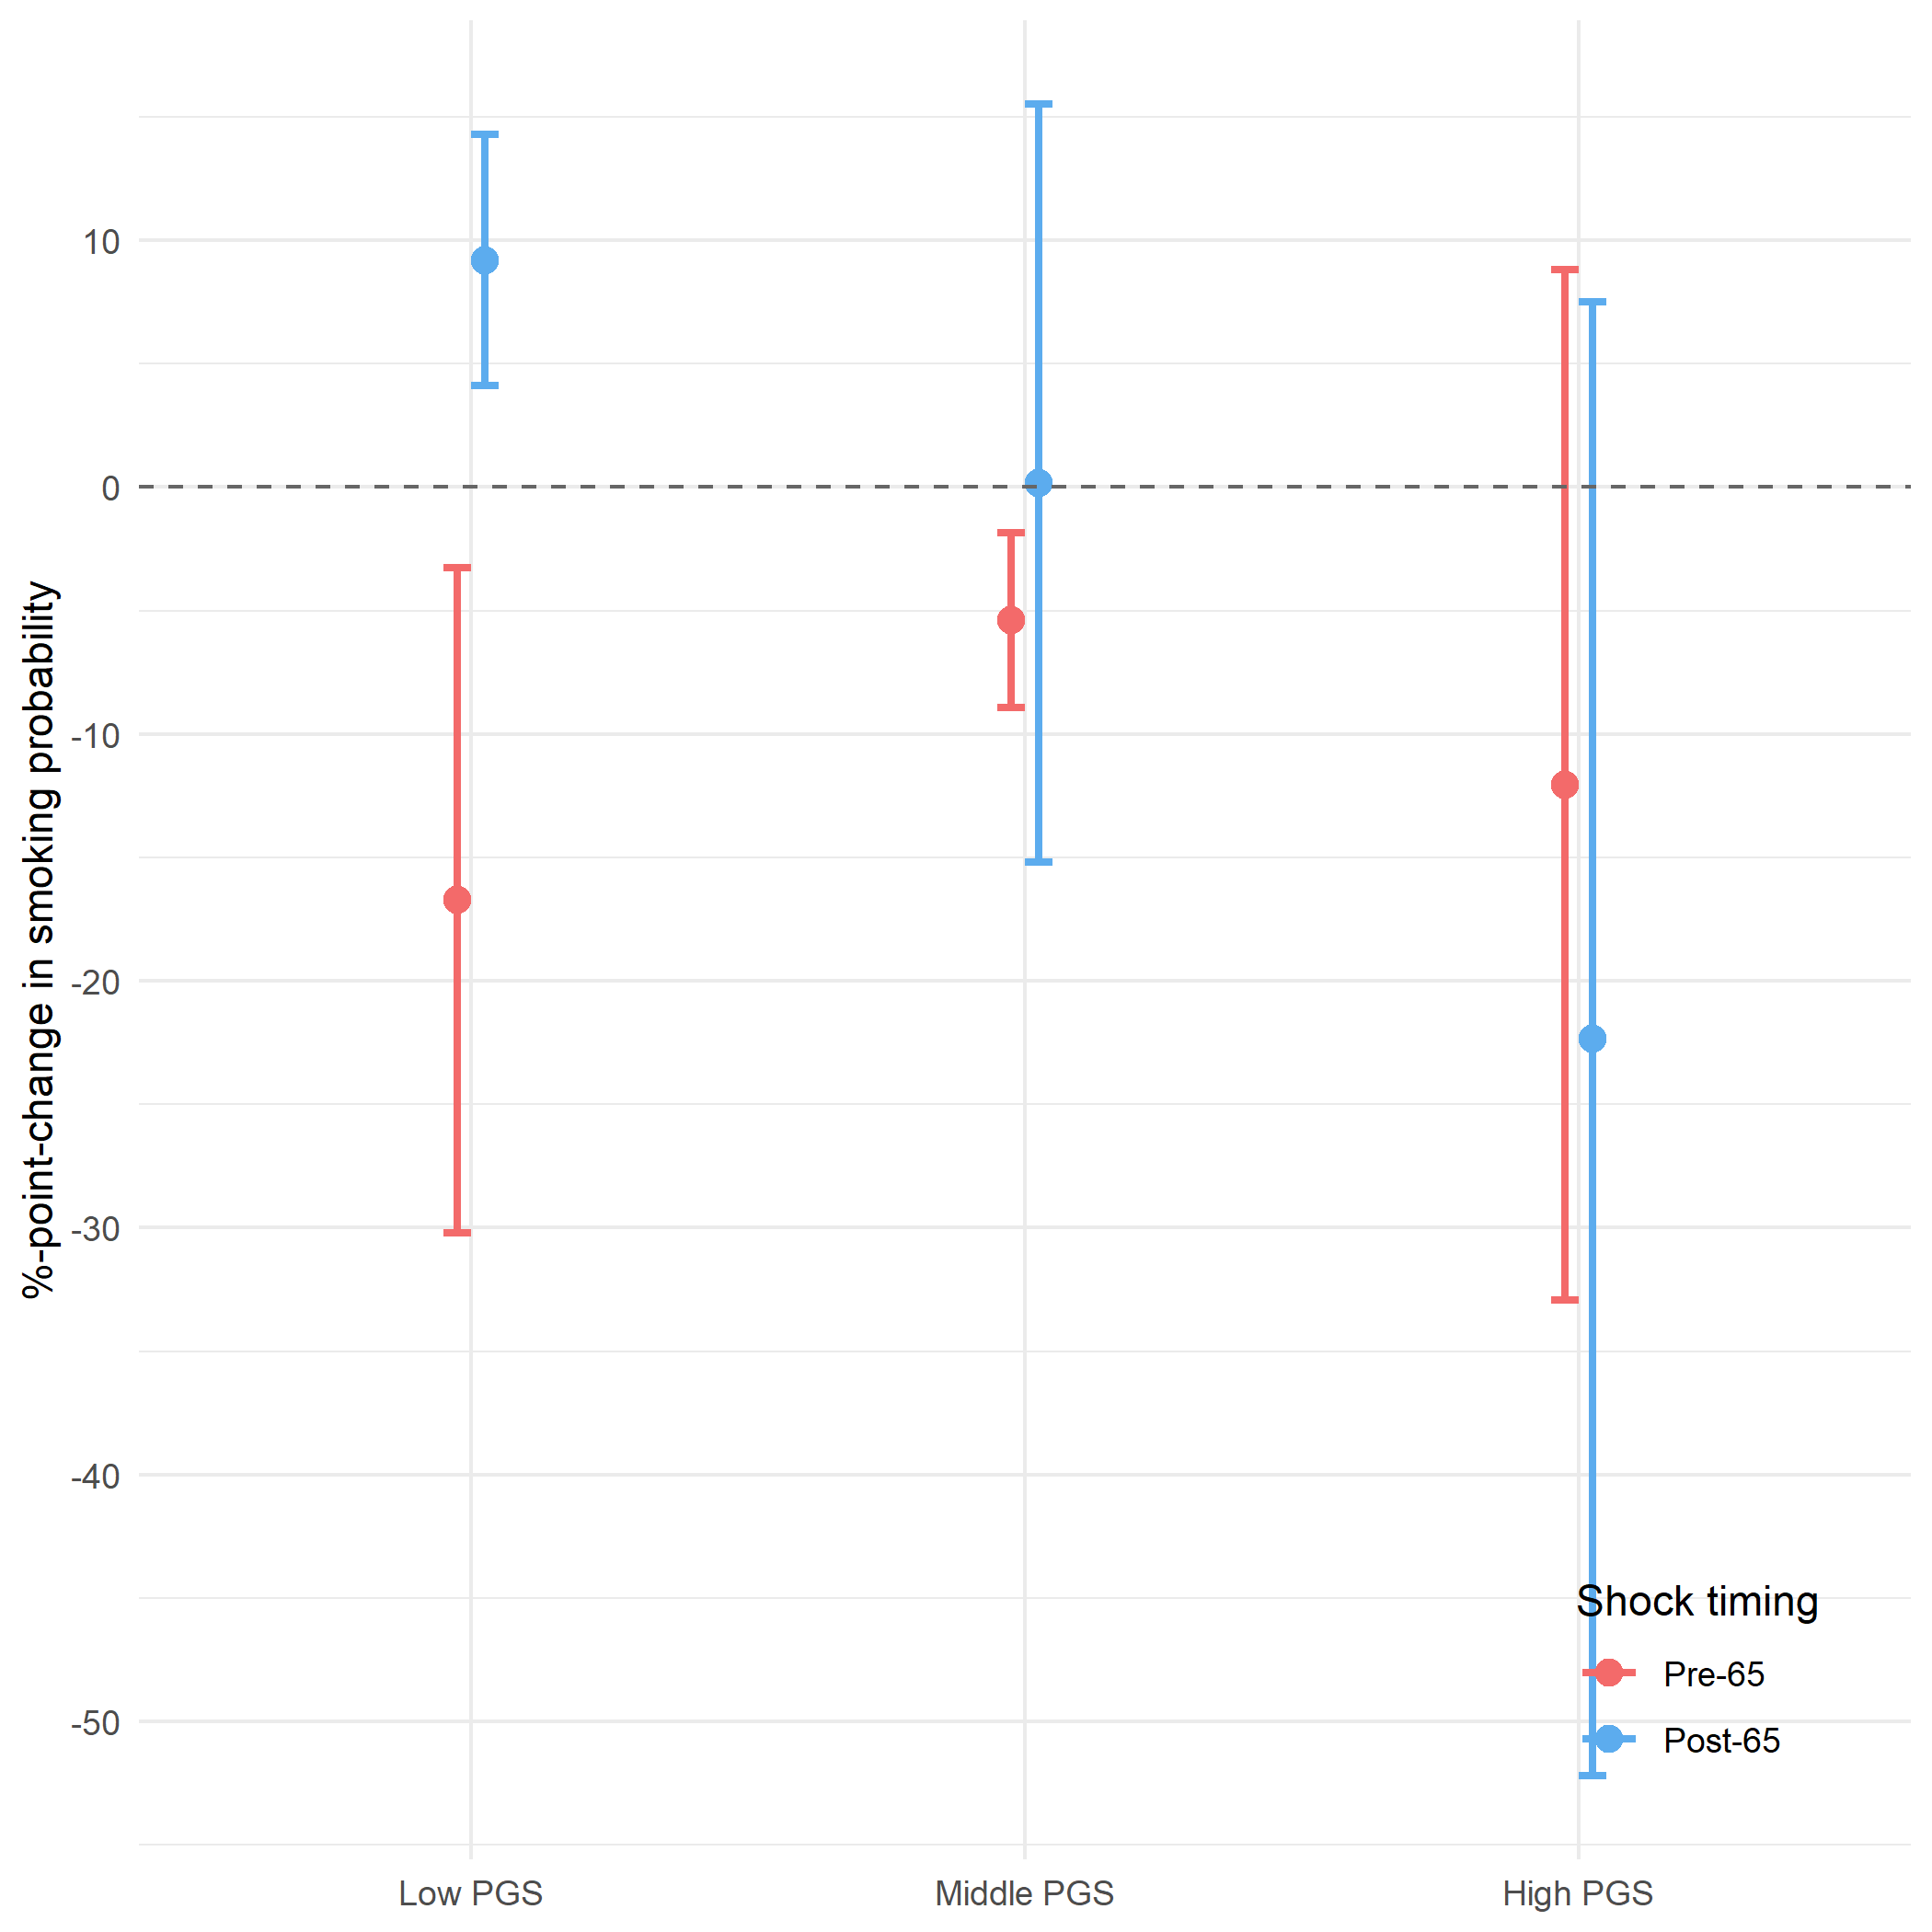
\includegraphics[width=0.8\textwidth]{../3_output/shock_effects/robustness_6070_3pgs_cv.png}
		\caption{Effect of a Health Shock on the Smoking Probability in the Pre-65 Uninsured Subgroup, Stratified by Timing of the Shock and Genetic Type (median split)
		\label{fig:3pgs}
		}
	\vspace{-0.8cm}
	\floatfoot{
	\textsf{
	\textit{Notes:} Low PGS = lowest tertile of the polygenic score distribution;
	Middle PGS = high PGS = upper two tertiles of the polygenic score distribution.
	Pre-65: Health shock since the last survey reported at ages 60-64.
	Post-65: Health shock since the last survey reported at ages 67-70.
	Estimates and standard errors are shown in Panel A of Table \ref{tab:main_effects}.
	Effects are estimated using the coefficients in Table \ref{tab:reg_results_multi} and following the derivation described in \ref{appsec:derivation}.
	Bars show 95\% confidence intervals, standard error clustered at the individual level.
	\\ \textit{Data used}: HRS study sample, n = 5,854.
Supplement.
	} %end of textsf
	} %end of floatfoot
	\end{center}
\end{figure}


\subsubsection{Median Split of the polygenic score} \label{appsec:median}

In this section, we derive the results by using a median-split for the PGS, instead of tertiles.
Results shown in Tables \ref{tab:reg_results_multi_median} \ref{tab:median_effects}, as well as Figure \ref{fig:shock_effects_median}, show that the effects are virtually the same, albeit a bit smaller in magnitude and less precisely estimated, as when splitting the PGS according to tertiles.

%\captionsetup{width = 9cm}
\begin{table}[!ht] \centering
	\caption{Coefficients from estimating the linear probability model in equation (\ref{eq:regression}) using OLS (PGS median split) \vspace{-0.4cm}}
	\addtolength{\tabcolsep}{-7pt}
	\label{tab:reg_results_multi_median}
	\resizebox{0.60\textheight}{!}{
	
% Table created by stargazer v.5.2.2 by Marek Hlavac, Harvard University. E-mail: hlavac at fas.harvard.edu
% Date and time: Wed, Dec 09, 2020 - 11:30:49 PM
% Requires LaTeX packages: dcolumn 
\begin{tabular}{@{\extracolsep{0pt}}lD{.}{.}{-3} D{.}{.}{-3} D{.}{.}{-3} D{.}{.}{-3} D{.}{.}{-3} } 
\\[-1.8ex]\hline 
\hline \\[-1.8ex] 
 & \multicolumn{5}{c}{\textit{Dependent variable:}} \\ 
\cline{2-6} 
\\[-1.8ex] & \multicolumn{5}{c}{Smoking status} \\ 
\\[-1.8ex] & \multicolumn{1}{c}{(1)} & \multicolumn{1}{c}{(2)} & \multicolumn{1}{c}{(3)} & \multicolumn{1}{c}{(4)} & \multicolumn{1}{c}{(5)}\\ 
\hline \\[-1.8ex] 
 Health Shock & -0.034 & -0.034 & -0.033 & -0.048^{**} & -0.047^{**} \\ 
  & (0.031) & (0.032) & (0.031) & (0.019) & (0.019) \\ 
  & & & & & \\ 
 Post-65 & -0.066^{***} & -0.022^{*} & -0.021^{*} & -0.013^{*} & -0.012^{*} \\ 
  & (0.007) & (0.012) & (0.012) & (0.007) & (0.007) \\ 
  & & & & & \\ 
 Uninsured & 0.168^{***} & 0.169^{***} & 0.169^{***} &  &  \\ 
  & (0.027) & (0.027) & (0.027) &  &  \\ 
  & & & & & \\ 
 High PGS & 0.039^{***} & 0.040^{***} & 0.040^{***} &  &  \\ 
  & (0.012) & (0.012) & (0.012) &  &  \\ 
  & & & & & \\ 
 Shock $\times$ Post-65 & 0.017 & 0.024 & 0.024 & 0.019 & 0.019 \\ 
  & (0.045) & (0.045) & (0.046) & (0.028) & (0.028) \\ 
  & & & & & \\ 
 Shock $\times$ Uninsured & -0.055 & -0.055 & -0.056 & -0.071 & -0.073 \\ 
  & (0.160) & (0.160) & (0.159) & (0.048) & (0.048) \\ 
  & & & & & \\ 
 Post-65 $\times$ Uninsured & 0.026 & 0.025 & 0.025 & -0.045^{*} & -0.045^{*} \\ 
  & (0.036) & (0.037) & (0.037) & (0.025) & (0.025) \\ 
  & & & & & \\ 
 Shock $\times$ High PGS & 0.052 & 0.050 & 0.048 & 0.024 & 0.024 \\ 
  & (0.046) & (0.046) & (0.046) & (0.027) & (0.027) \\ 
  & & & & & \\ 
 Post-65 $\times$ High PGS & 0.004 & 0.004 & 0.003 & 0.0001 & -0.0003 \\ 
  & (0.010) & (0.010) & (0.010) & (0.007) & (0.007) \\ 
  & & & & & \\ 
 Shock $\times$ Post-65 x Uninsured & 0.090 & 0.090 & 0.090 & 0.136^{**} & 0.137^{**} \\ 
  & (0.212) & (0.213) & (0.212) & (0.067) & (0.067) \\ 
  & & & & & \\ 
 Shock $\times$ Uninsured $\times$ High PGS & 0.004 & 0.014 & 0.015 & -0.028 & -0.026 \\ 
  & (0.211) & (0.211) & (0.210) & (0.119) & (0.119) \\ 
  & & & & & \\ 
 Shock $\times$ Post-65 $\times$ High PGS & -0.082 & -0.078 & -0.077 & -0.086^{**} & -0.088^{**} \\ 
  & (0.064) & (0.064) & (0.064) & (0.042) & (0.042) \\ 
  & & & & & \\ 
 Post-65 $\times$ Uninsured $\times$ High PGS & -0.072 & -0.072 & -0.072 & 0.041 & 0.041 \\ 
  & (0.057) & (0.057) & (0.057) & (0.033) & (0.033) \\ 
  & & & & & \\ 
 Shock $\times$ Post-65 $\times$ Uninsured $\times$ High PGS & 0.154 & 0.145 & 0.142 & -0.131 & -0.136 \\ 
  & (0.310) & (0.312) & (0.311) & (0.189) & (0.188) \\ 
  & & & & & \\ 
\hline \\[-1.8ex] 
Age & & Yes & Yes & Yes & Yes  \\
Year FE & &              & Yes &              & Yes  \\
Individual FE   & &              &              & Yes & Yes  \\
 \hline \\[-1.8ex]
Observations & \multicolumn{1}{c}{26,022} & \multicolumn{1}{c}{26,022} & \multicolumn{1}{c}{26,022} & \multicolumn{1}{c}{26,022} & \multicolumn{1}{c}{26,022} \\ 
R$^{2}$ & \multicolumn{1}{c}{0.016} & \multicolumn{1}{c}{0.017} & \multicolumn{1}{c}{0.018} & \multicolumn{1}{c}{0.823} & \multicolumn{1}{c}{0.823} \\ 
\hline 
\hline \\[-1.8ex] 
\end{tabular} 

	} %end of resizebox
	\begin{flushleft}
	\textit{Notes:}
	Health shock = binary indicator for having suffered a cardiovascular health shock for the first time since the previous wave.
	Post-65 = indicator for age $>$ 65 at the time of the interview.
	Uninsured = binary indicator for being persistently uninsured in every observation of the study sample before the age of 65.
	High PGS = indicator for being above the median polygenic score.
    Age = controls for 3$^{rd}$ degree polynomial in age.
    FE = adding fixed effects.
	Robust standard errors in parentheses are clustered at the individual level.
	$^{*}$p$<$0.1; $^{**}$p$<$0.05; $^{***}$p$<$0.01.
	\\ \textit{Data used}: HRS study sample, n = 5,854.
	\end{flushleft}
\end{table}


%%\captionsetup{width = 9cm}
\begin{table*}[!ht]
	\caption{Summary of Statistical Results for the Pre-65 Uninsured Subgroup, Stratified by Timing of the Shock and Genetic Group (Median)}
	\label{tab:median_effects}
	%\resizebox{7.5cm}{!}{
	% latex table generated in R 4.0.2 by xtable 1.8-4 package
% 
\begin{tabular}{lll}
  \toprule
  \multicolumn{3}{c}{ \textbf{Effect of health shock on smoking probability}} \\
 \midrule
 & Low PGS & High PGS \\ 
   \midrule
Pre 65 & -0.122*** & -0.121 \\ 
   & (0.044) & (0.107) \\ 
  Post 65 & 0.037 & -0.139 \\ 
   & (0.041) & (0.132) \\ 
   \toprule \multicolumn{3}{c}{ \textbf{Effect of health insurance on effect of health shock}} \\
 \midrule
 & Low PGS & High PGS \\ 
   \midrule
Post 65 - Pre 65 & 0.158*** & -0.017 \\ 
   & (0.061) & (0.169) \\ 
   \toprule \multicolumn{3}{c}{ \textbf{Differential effect of health insurance by genetic group}} \\
 \midrule
 & High PGS  & - low PGS \\ 
   \midrule
Post 65 - Pre 65 & -0.176 &  \\ 
   & (0.18) &  \\ 
   \bottomrule
\end{tabular}

		\begin{flushleft}
			Low PGS = polygenic score below the median; high PGS = polygenic score above the median.
			Pre-65: Health shock since the last survey reported at ages 60-64.
			Post-65: Health shock since the last survey reported at ages 67-70.
			$^{*}$P $<$ 0.1; $^{**}$P $<$ 0.05; $^{***}$P $<$ 0.01. Robust standard errors in parentheses are clustered at the individual level.
			The covariance matrix used for calculating standard errors is shown in Appendix Table \ref{suptab:cov_matrix}.
			Effects are estimated using the coefficients in Table \ref{tab:reg_results_multi} and following the derivation described in \ref{appsec:derivation}.\\
			\textit{Data used}: HRS study sample, n = 5,854.
			%Composition of all effects is shown in Tables \ref{suptab:main_explained}, \ref{suptab:main_explained2}, and \ref{suptab:main_explained3} in the Supplement.
		\end{flushleft}
	%\headrule
\end{table*}




%\captionsetup{width = \columnwidth}
\begin{figure}[!ht]
	\begin{center}
		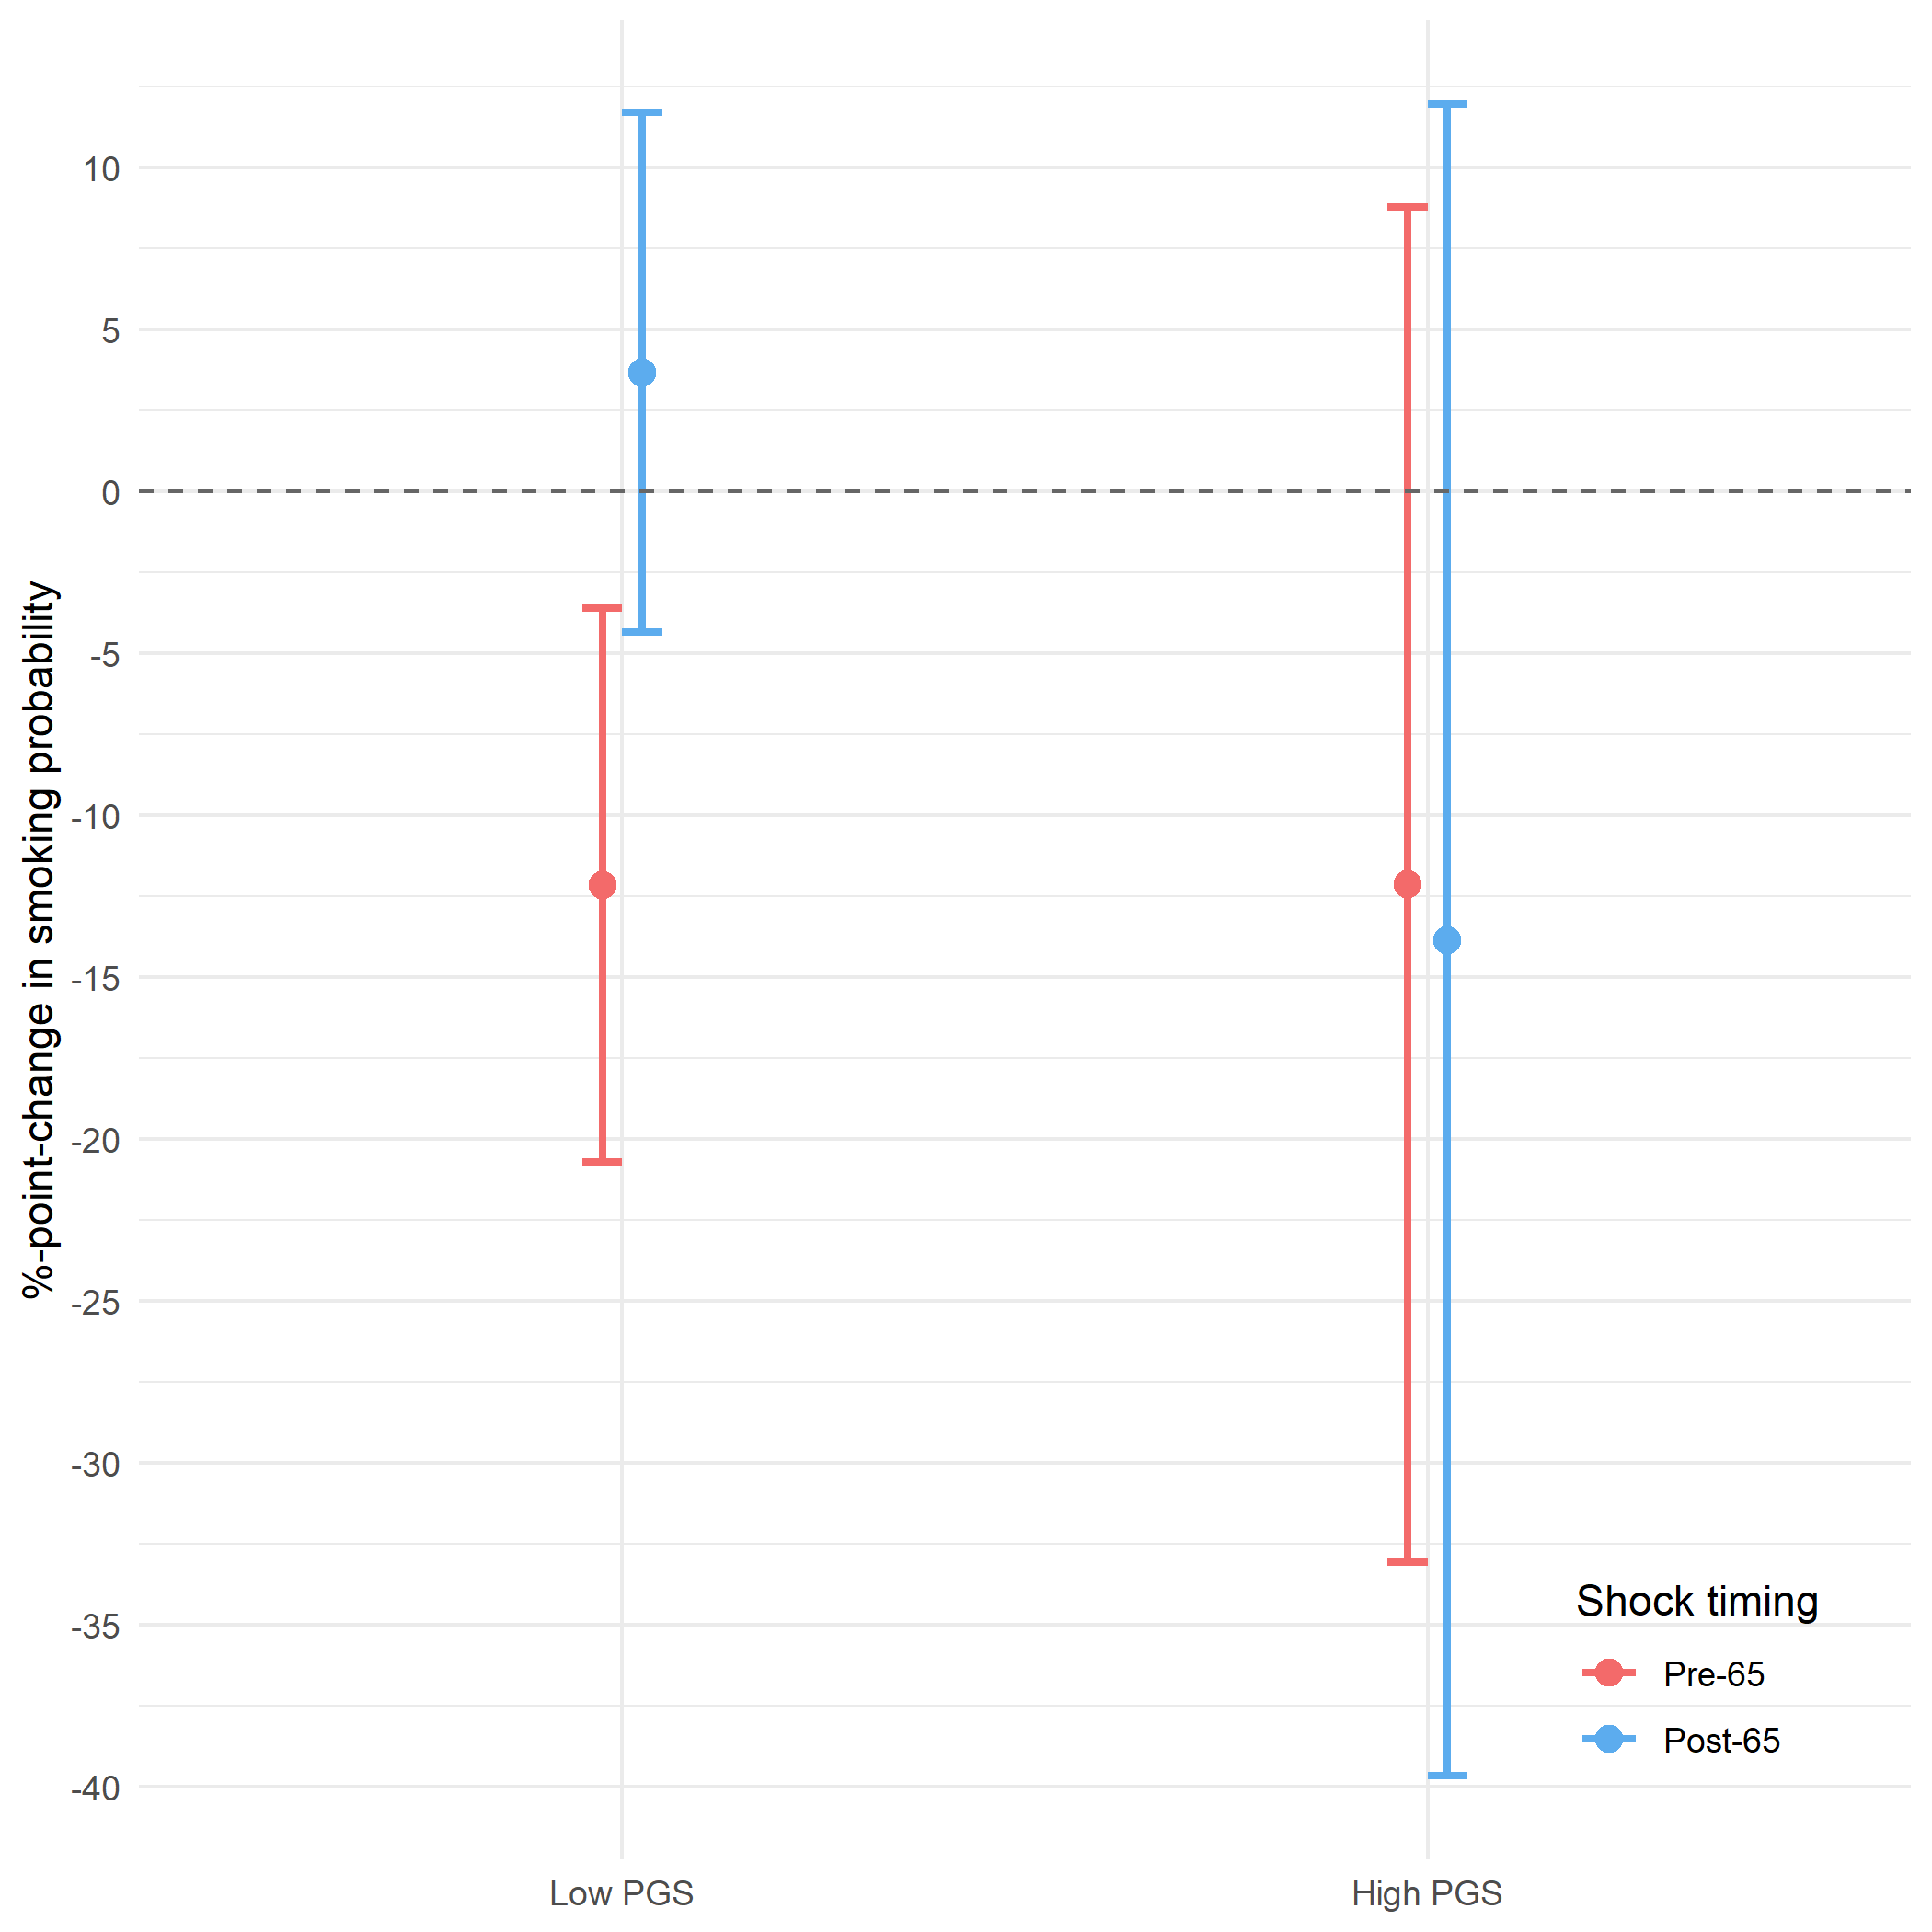
\includegraphics[width=0.8\textwidth]{../3_output/shock_effects/main_6070_100_cv_Median.png}
		\caption{Effect of a Health Shock on the Smoking Probability in the Pre-65 Uninsured Subgroup, Stratified by Timing of the Shock and Genetic Type (median split)
		\label{fig:shock_effects_median}
		}
	\vspace{-0.8cm}
	\floatfoot{
	\textsf{
	\textit{Notes:} Low PGS = polygenic score below the median; high PGS = polygenic score above the median.
	Pre-65: Health shock since the last survey reported at ages 60-64.
	Post-65: Health shock since the last survey reported at ages 67-70.
	Estimates and standard errors are shown in Panel A of Table \ref{tab:main_effects}.
	Effects are estimated using the coefficients in Table \ref{tab:reg_results_multi} and following the derivation described in \ref{appsec:derivation}.
	Bars show 95\% confidence intervals, standard error clustered at the individual level.
	\\ \textit{Data used}: HRS study sample, n = 5,854.
	%Composition of all effects is shown in Tables \ref{suptab:main_explained}, \ref{suptab:main_explained2}, and \ref{suptab:main_explained3} in the Supplement.
	} %end of textsf
	} %end of floatfoot
	\end{center}
\end{figure}

\subsubsection{Older GWAS Summary Statistics} \label{appsec:TAG2010}

In this section, we also use the polygenic score publicly provided by the HRS \citep{HRSPGenscore2017} for the smoking phenotype ``regular smoking'' (having smoked more than 100 cigarettes throughout one's life).
This score is constructed as a weighted sum of the genotype over the 779,538 SNPs that overlap between the HRS genetic database and a 2010 GWAS meta-analysis conducted by the Tobacco and Genetics Consortium \citep{TAG2010}.

Results shown in Tables \ref{tab:oldpgs_effects} and Figure \ref{fig:shock_effects_oldpgs}, show that the effects are virtually the same, possibly even a bit stronger.

%%\captionsetup{width = 9cm}
\begin{table*}[!ht]
	\caption{Summary of Statistical Results for the Pre-65 Uninsured Subgroup, Stratified by Timing of the Shock and Genetic Group (older PGS)}
	\label{tab:oldpgs_effects}
	%\resizebox{7.5cm}{!}{
	% latex table generated in R 4.0.2 by xtable 1.8-4 package
% 
\begin{tabular}{lll}
  \toprule
  \multicolumn{3}{c}{ \textbf{Effect of health shock on smoking probability}} \\
 \midrule
 & Low PGS & High PGS \\ 
   \midrule
Pre 65 & -0.338** & -0.018 \\ 
   & (0.135) & (0.128) \\ 
  Post 65 & 0.06*** & -0.12 \\ 
   & (0.02) & (0.105) \\ 
   \toprule \multicolumn{3}{c}{ \textbf{Effect of health insurance on effect of health shock}} \\
 \midrule
 & Low PGS & High PGS \\ 
   \midrule
Post 65 - Pre 65 & 0.399*** & -0.103 \\ 
   & (0.139) & (0.163) \\ 
   \toprule \multicolumn{3}{c}{ \textbf{Differential effect of health insurance by genetic group}} \\
 \midrule
 & High PGS  & - low PGS \\ 
   \midrule
Post 65 - Pre 65 & -0.501** &  \\ 
   & (0.214) &  \\ 
   \bottomrule
\end{tabular}

		\begin{flushleft}
			Low PGS = polygenic score below the median; high PGS = polygenic score above the median, constructed using the summary statistics from the Tobacco and Genetics Consortium \citep{TAG2010} (PGS publicly available from the HRS website).
			Pre-65: Health shock since the last survey reported at ages 60-64.
			Post-65: Health shock since the last survey reported at ages 67-70.
			$^{*}$P $<$ 0.1; $^{**}$P $<$ 0.05; $^{***}$P $<$ 0.01. Robust standard errors in parentheses are clustered at the individual level.
			The covariance matrix used for calculating standard errors is shown in Appendix Table \ref{suptab:cov_matrix}.
			Effects are estimated using the coefficients in Table \ref{tab:reg_results_multi} and following the derivation described in \ref{appsec:derivation}.\\
			\textit{Data used}: HRS study sample, n = 5,854.
			%Composition of all effects is shown in Tables \ref{suptab:main_explained}, \ref{suptab:main_explained2}, and \ref{suptab:main_explained3} in the Supplement.
		\end{flushleft}
	%\headrule
\end{table*}




%\captionsetup{width = \columnwidth}
\begin{figure}[!ht]
	\begin{center}
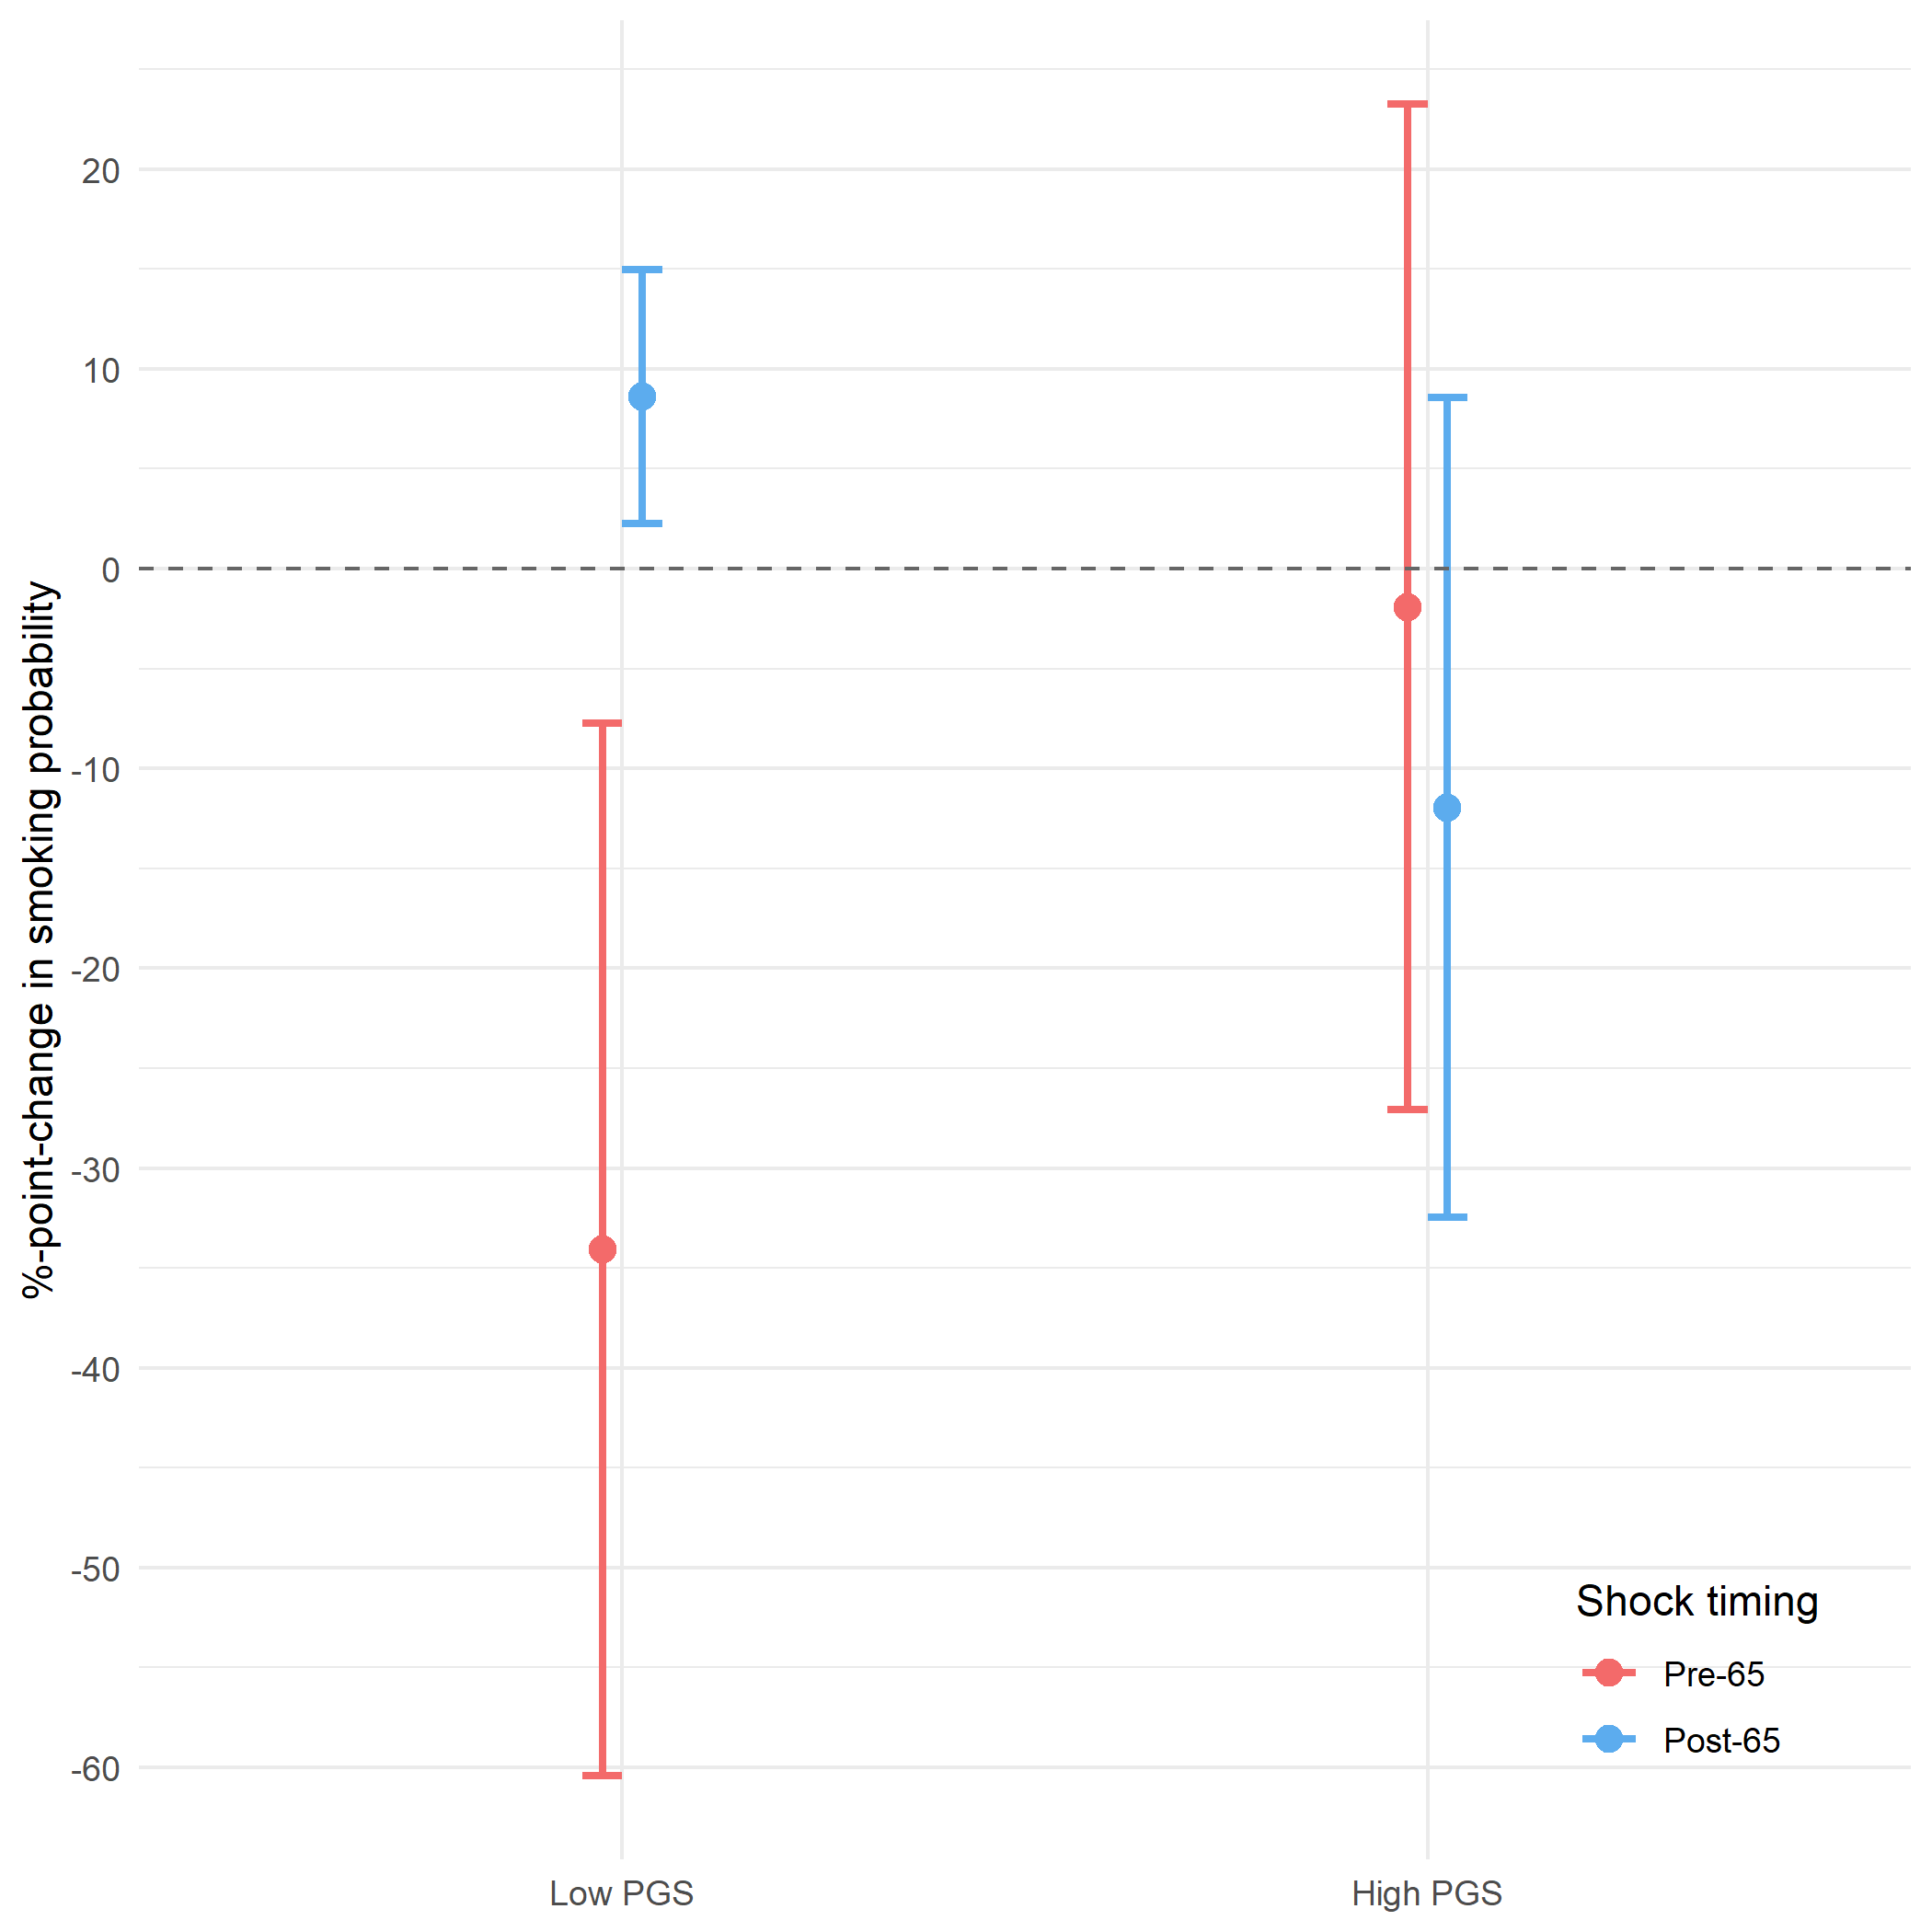
\includegraphics[width=0.6\textwidth]{../3_output/shock_effects/robustness_6070_oldpgs_cv.png}
		\caption{Effect of a Health Shock on the Smoking Probability in the Pre-65 Uninsured Subgroup, Stratified by Timing of the Shock and Genetic Type (older PGS)
		\label{fig:shock_effects_oldpgs}
		}
	\vspace{-0.8cm}
	\floatfoot{
	\textsf{
	\textit{Notes:} Low PGS = polygenic score below the median; high PGS = polygenic score above the median.
	Pre-65: Health shock since the last survey reported at ages 60-64.
	Post-65: Health shock since the last survey reported at ages 67-70.
	Estimates and standard errors are shown in Panel A of Table \ref{tab:main_effects}.
	Effects are estimated using the coefficients in Table \ref{tab:reg_results_multi} and following the derivation described in \ref{appsec:derivation}.
	Bars show 95\% confidence intervals, standard error clustered at the individual level.
	\\ \textit{Data used}: HRS study sample, n = 5,854.
	%Composition of all effects is shown in Tables \ref{suptab:main_explained}, \ref{suptab:main_explained2}, and \ref{suptab:main_explained3} in the Supplement.
	} %end of textsf
	} %end of floatfoot
	\end{center}
\end{figure}


%--------------------------------------------------------
\subsubsection{Using different polygenic scores} \label{appsec:otherPGS}
Other polygenic scores (PGS), besides the one for being a smoker, might be driving this heterogeneity in moral hazard.
We estimated the same analysis outlined in equation \ref{eq:regression} but replacing $g_i$ with the following PGS:
the PGS for cigarettes per day (CPD) \citep{GSCAN2019gwas}, the PGS for educational attainment and the one for cognitive abilities \citep{Lee2018}, the PGS for risk tolerance \citep{KarlssonLinner2019}, the PGS for non-cognitive skills \citep{Demange2020}, and the PGS for Body-Mass-Index \citep{Yengo2018}.
We chose polygenic scores for traits that are genetically correlated with smoking, such as CPD and risk tolerance, or plausibly related to strategic behaviors and moral hazard, such as education, cognition, and non-cognitive skills. BMI is meant more as a placebo.

\begin{figure}[ht]
	\begin{center}
		\subfigure[\textsf{PGS cigarettes per day}]
		{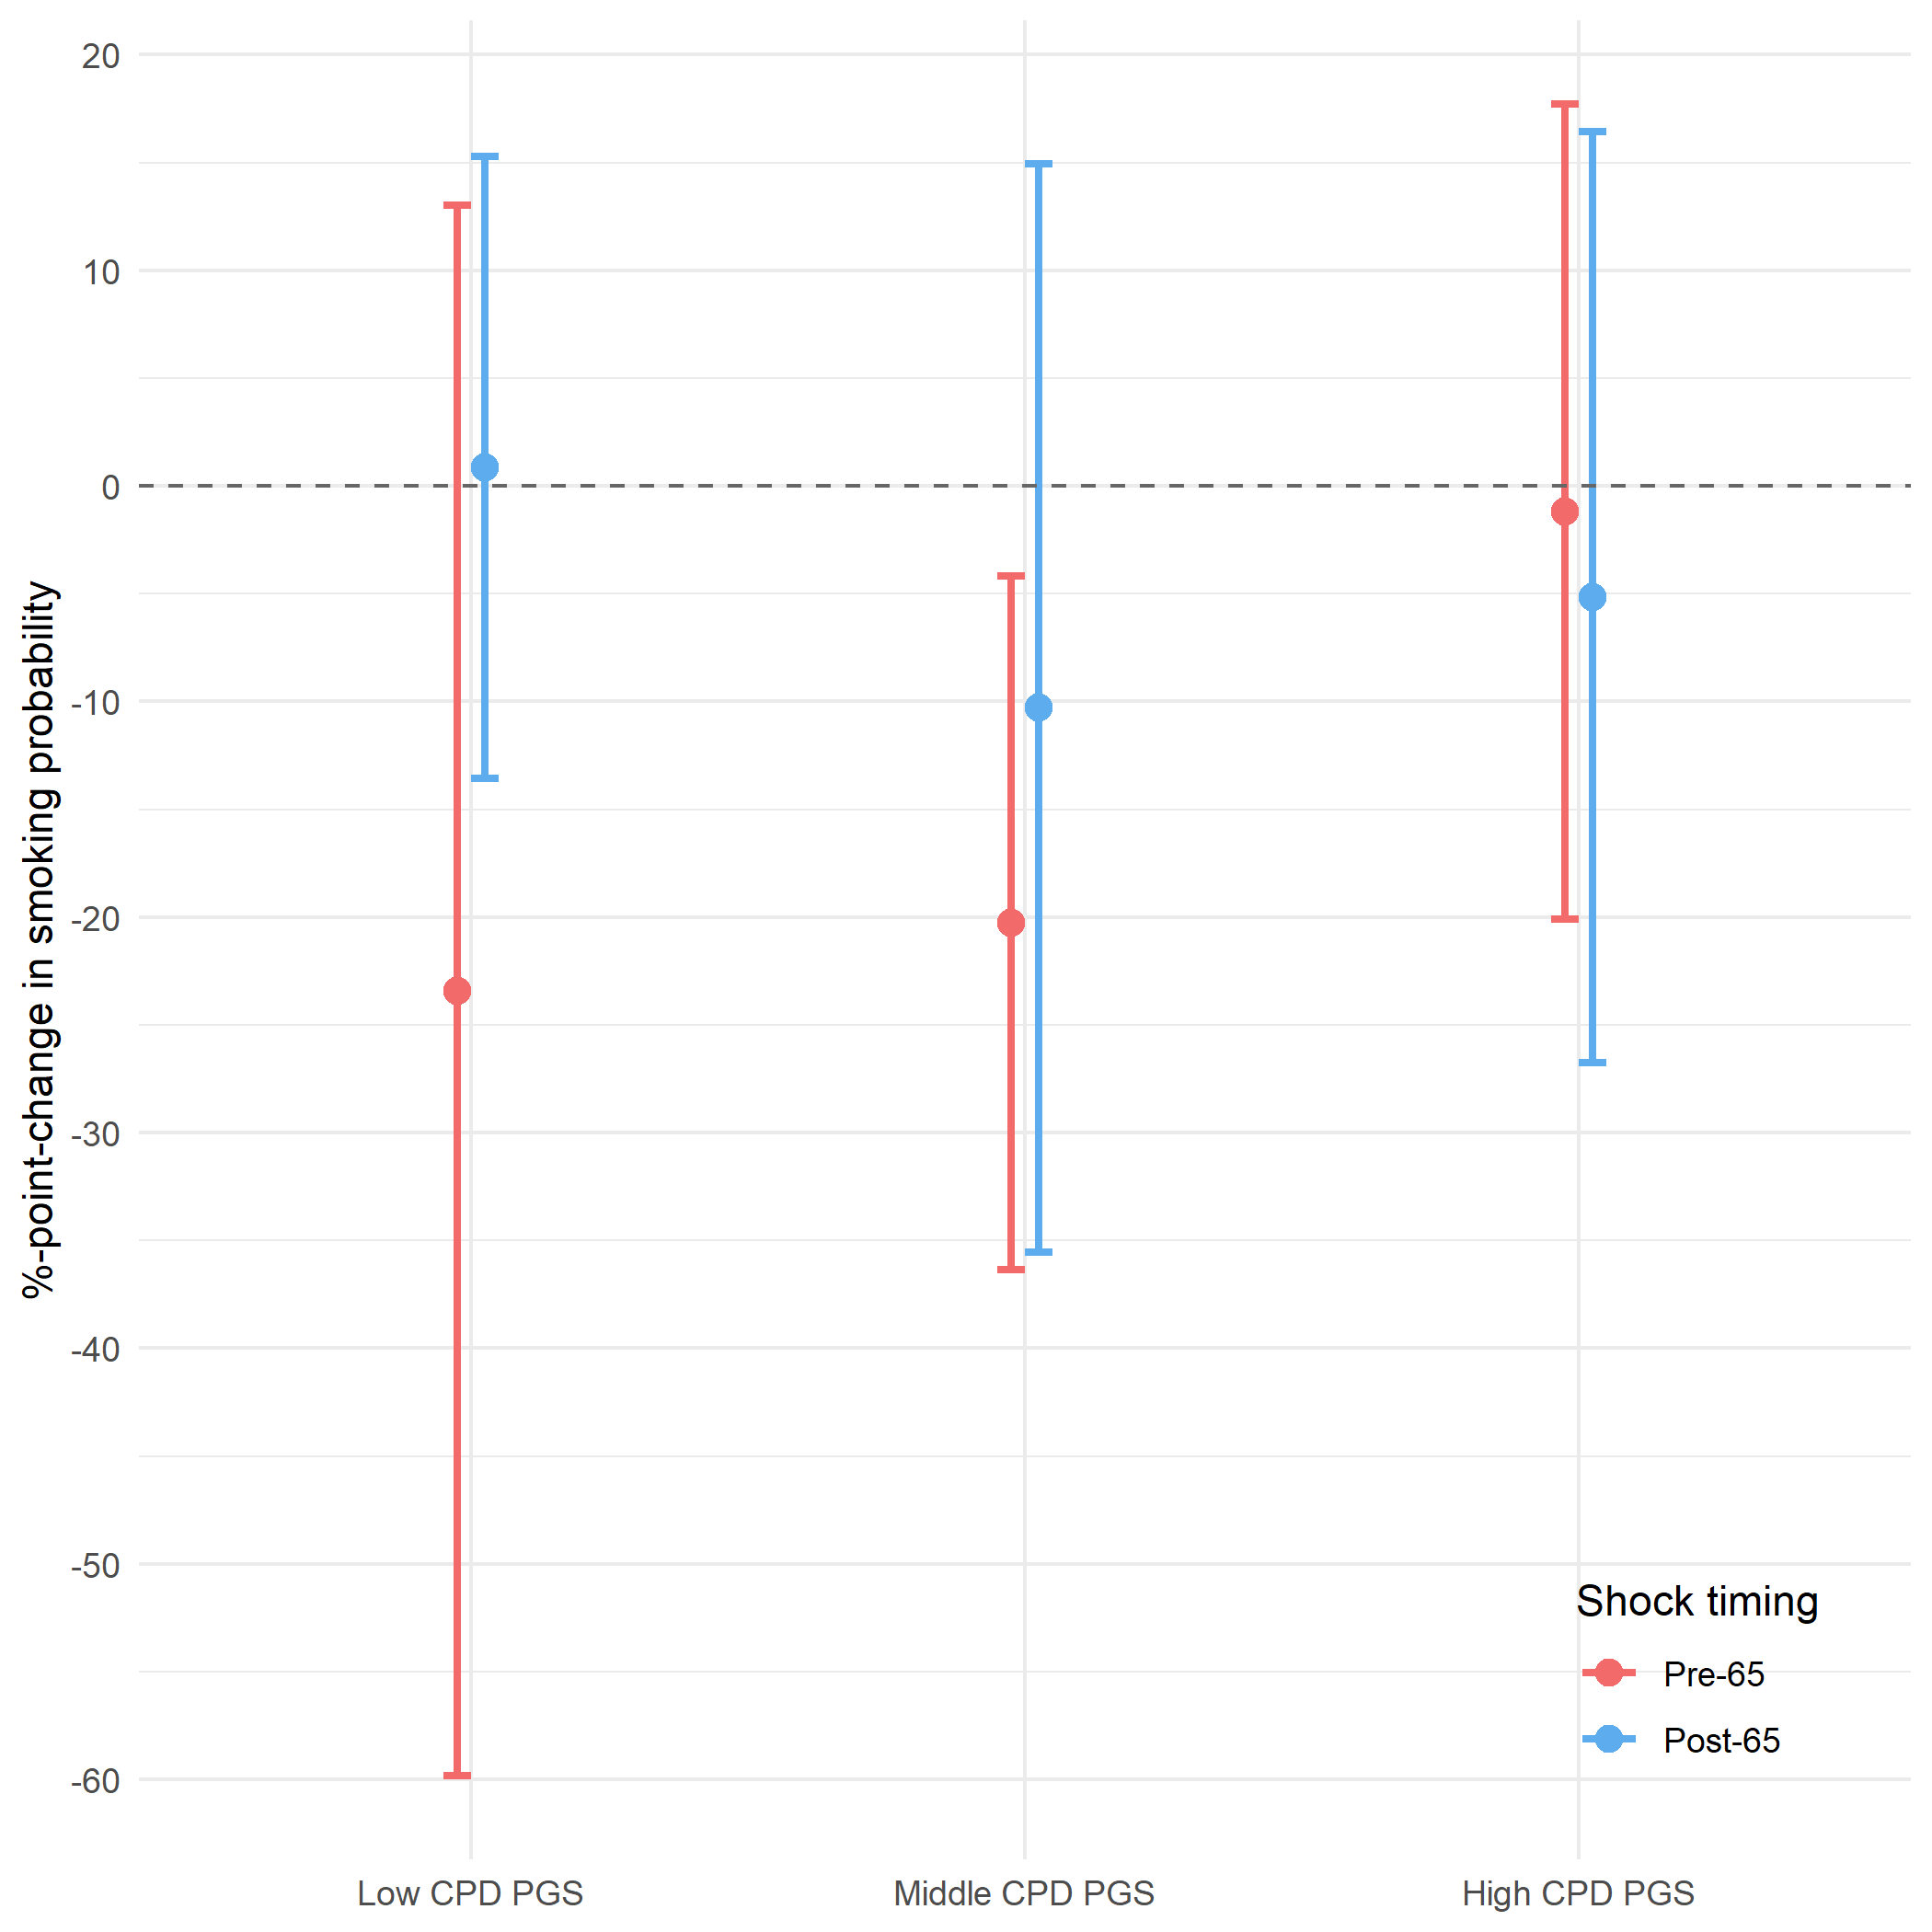
\includegraphics[width=0.3\textwidth]
		{../3_output/shock_effects/cpdPGS_6070_100_cv.png}
		}
		\subfigure[\textsf{PGS for educational attainment}]
		{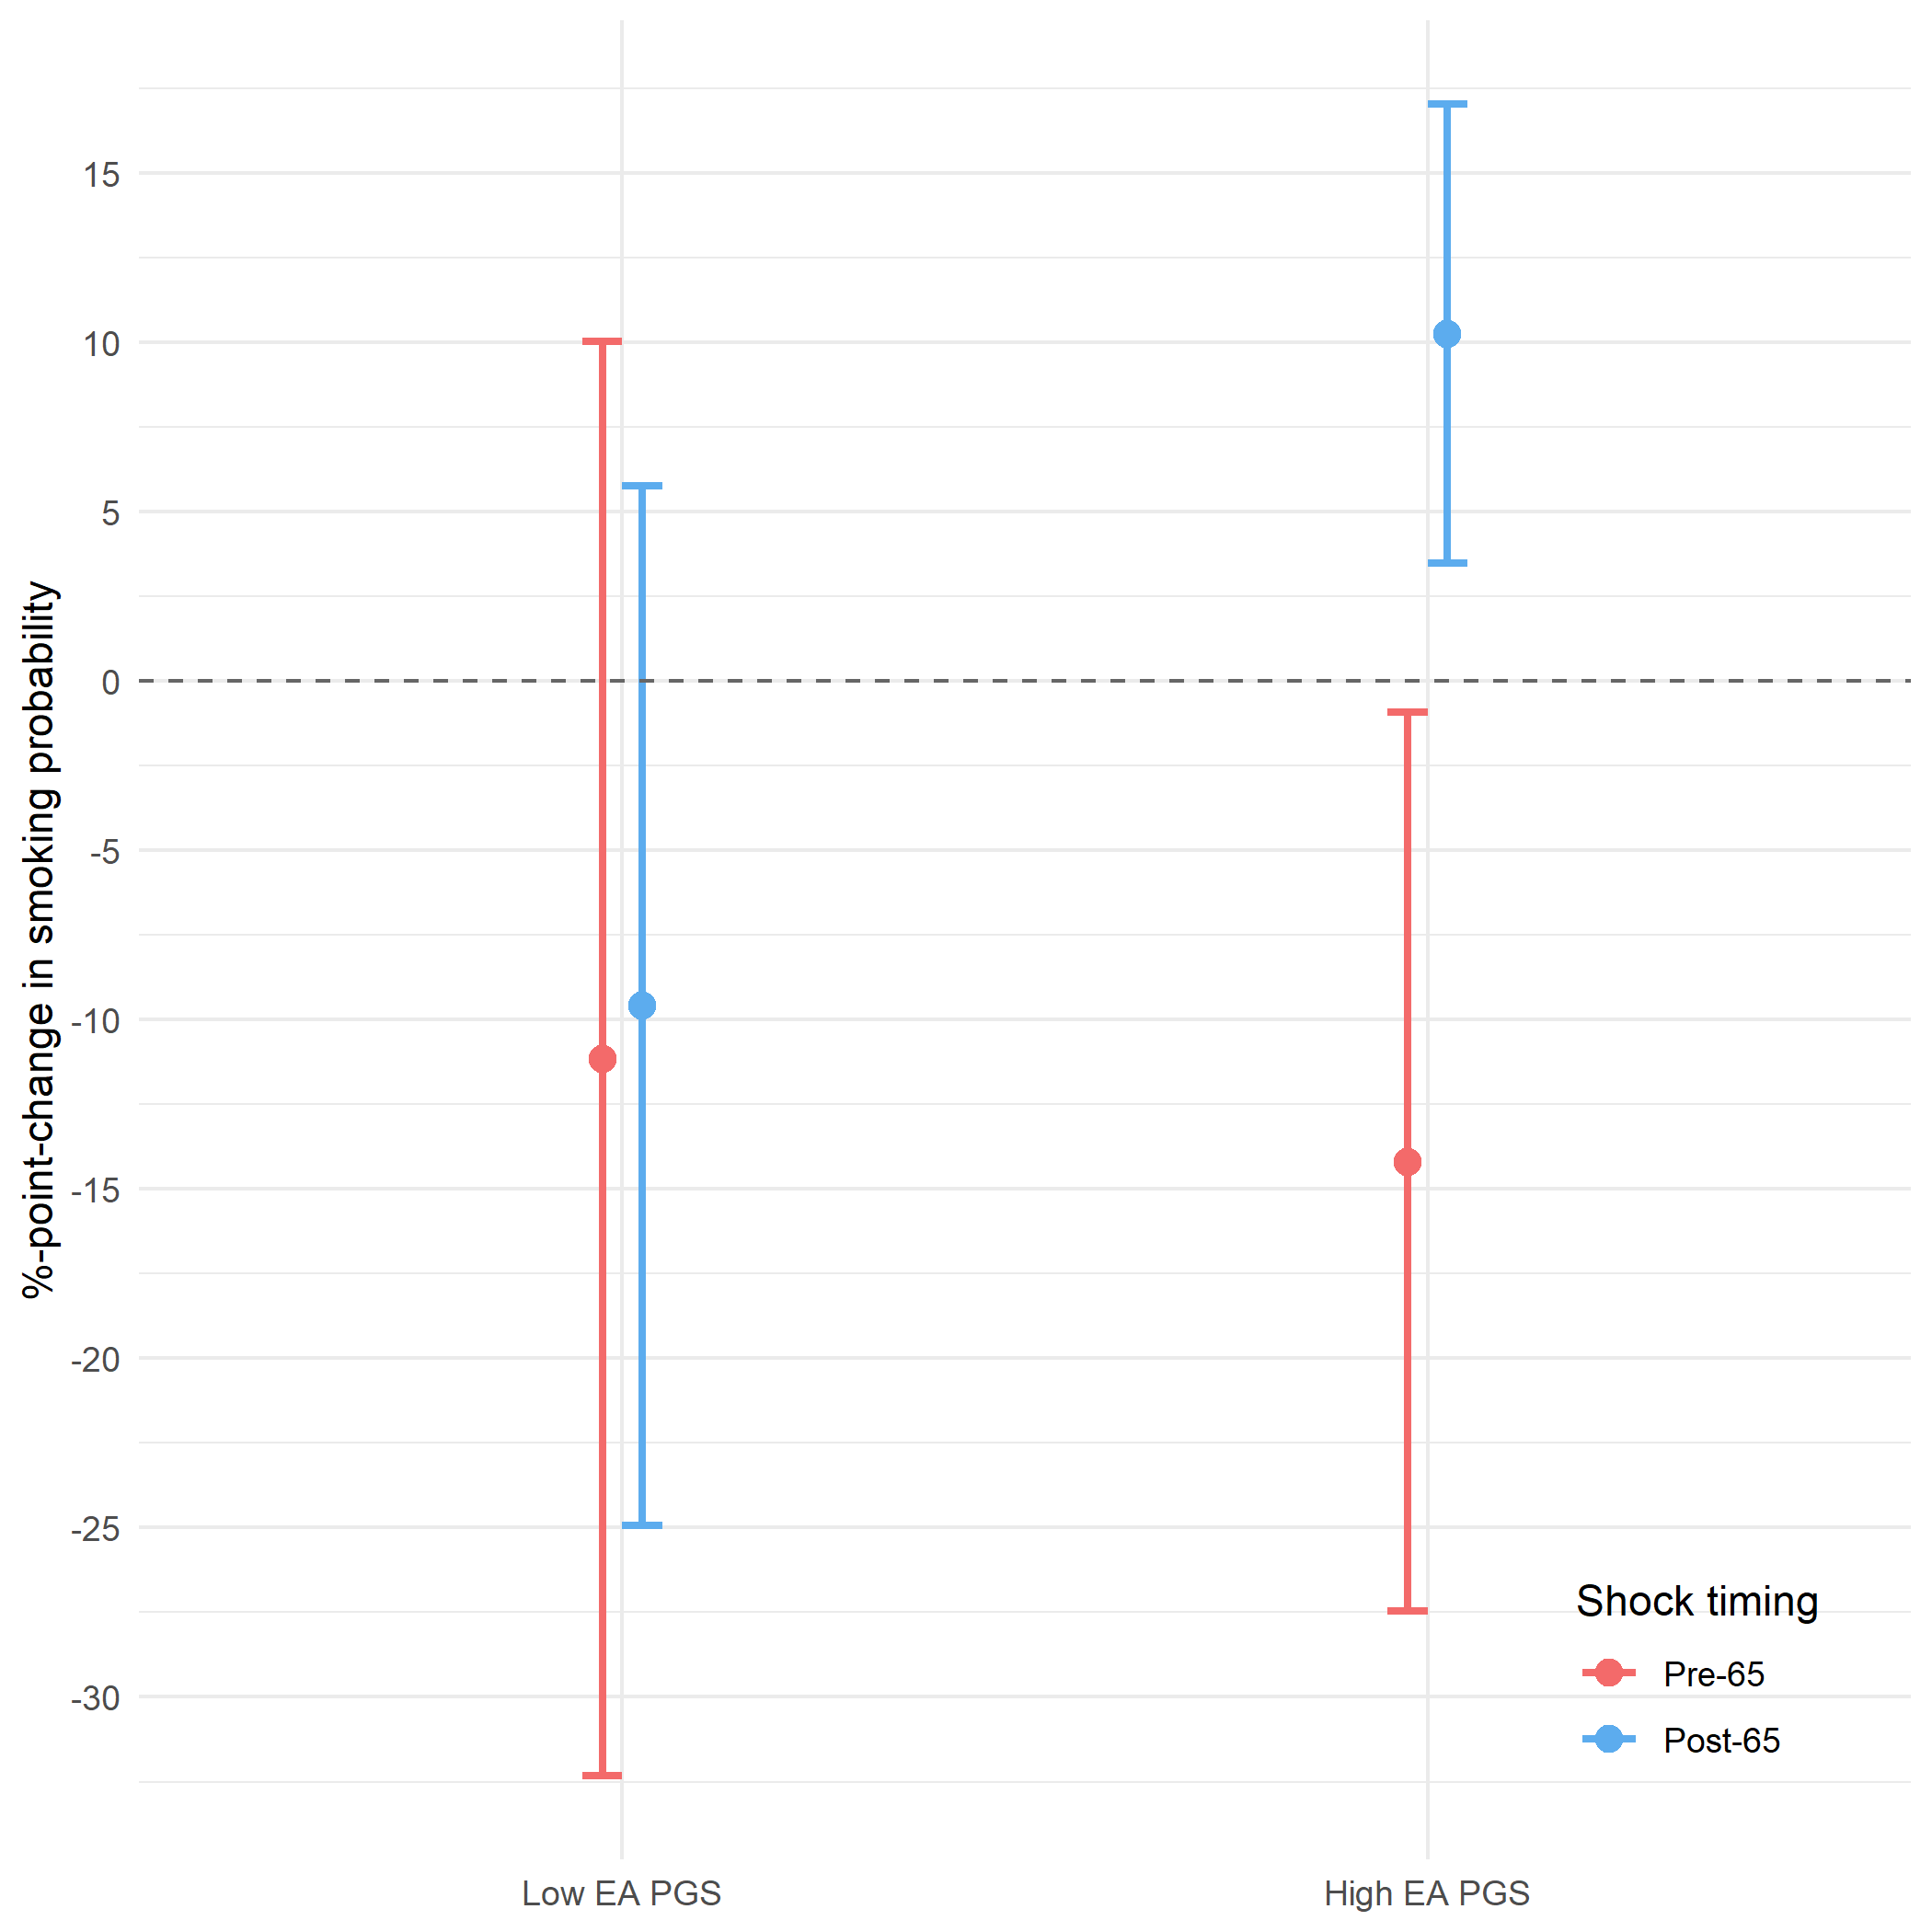
\includegraphics[width=0.3\textwidth]
		{../3_output/shock_effects/robustness_eaPGS_6070_100_cv.png}
		}
		\subfigure[\textsf{PGS for cognitive abilities}]
		{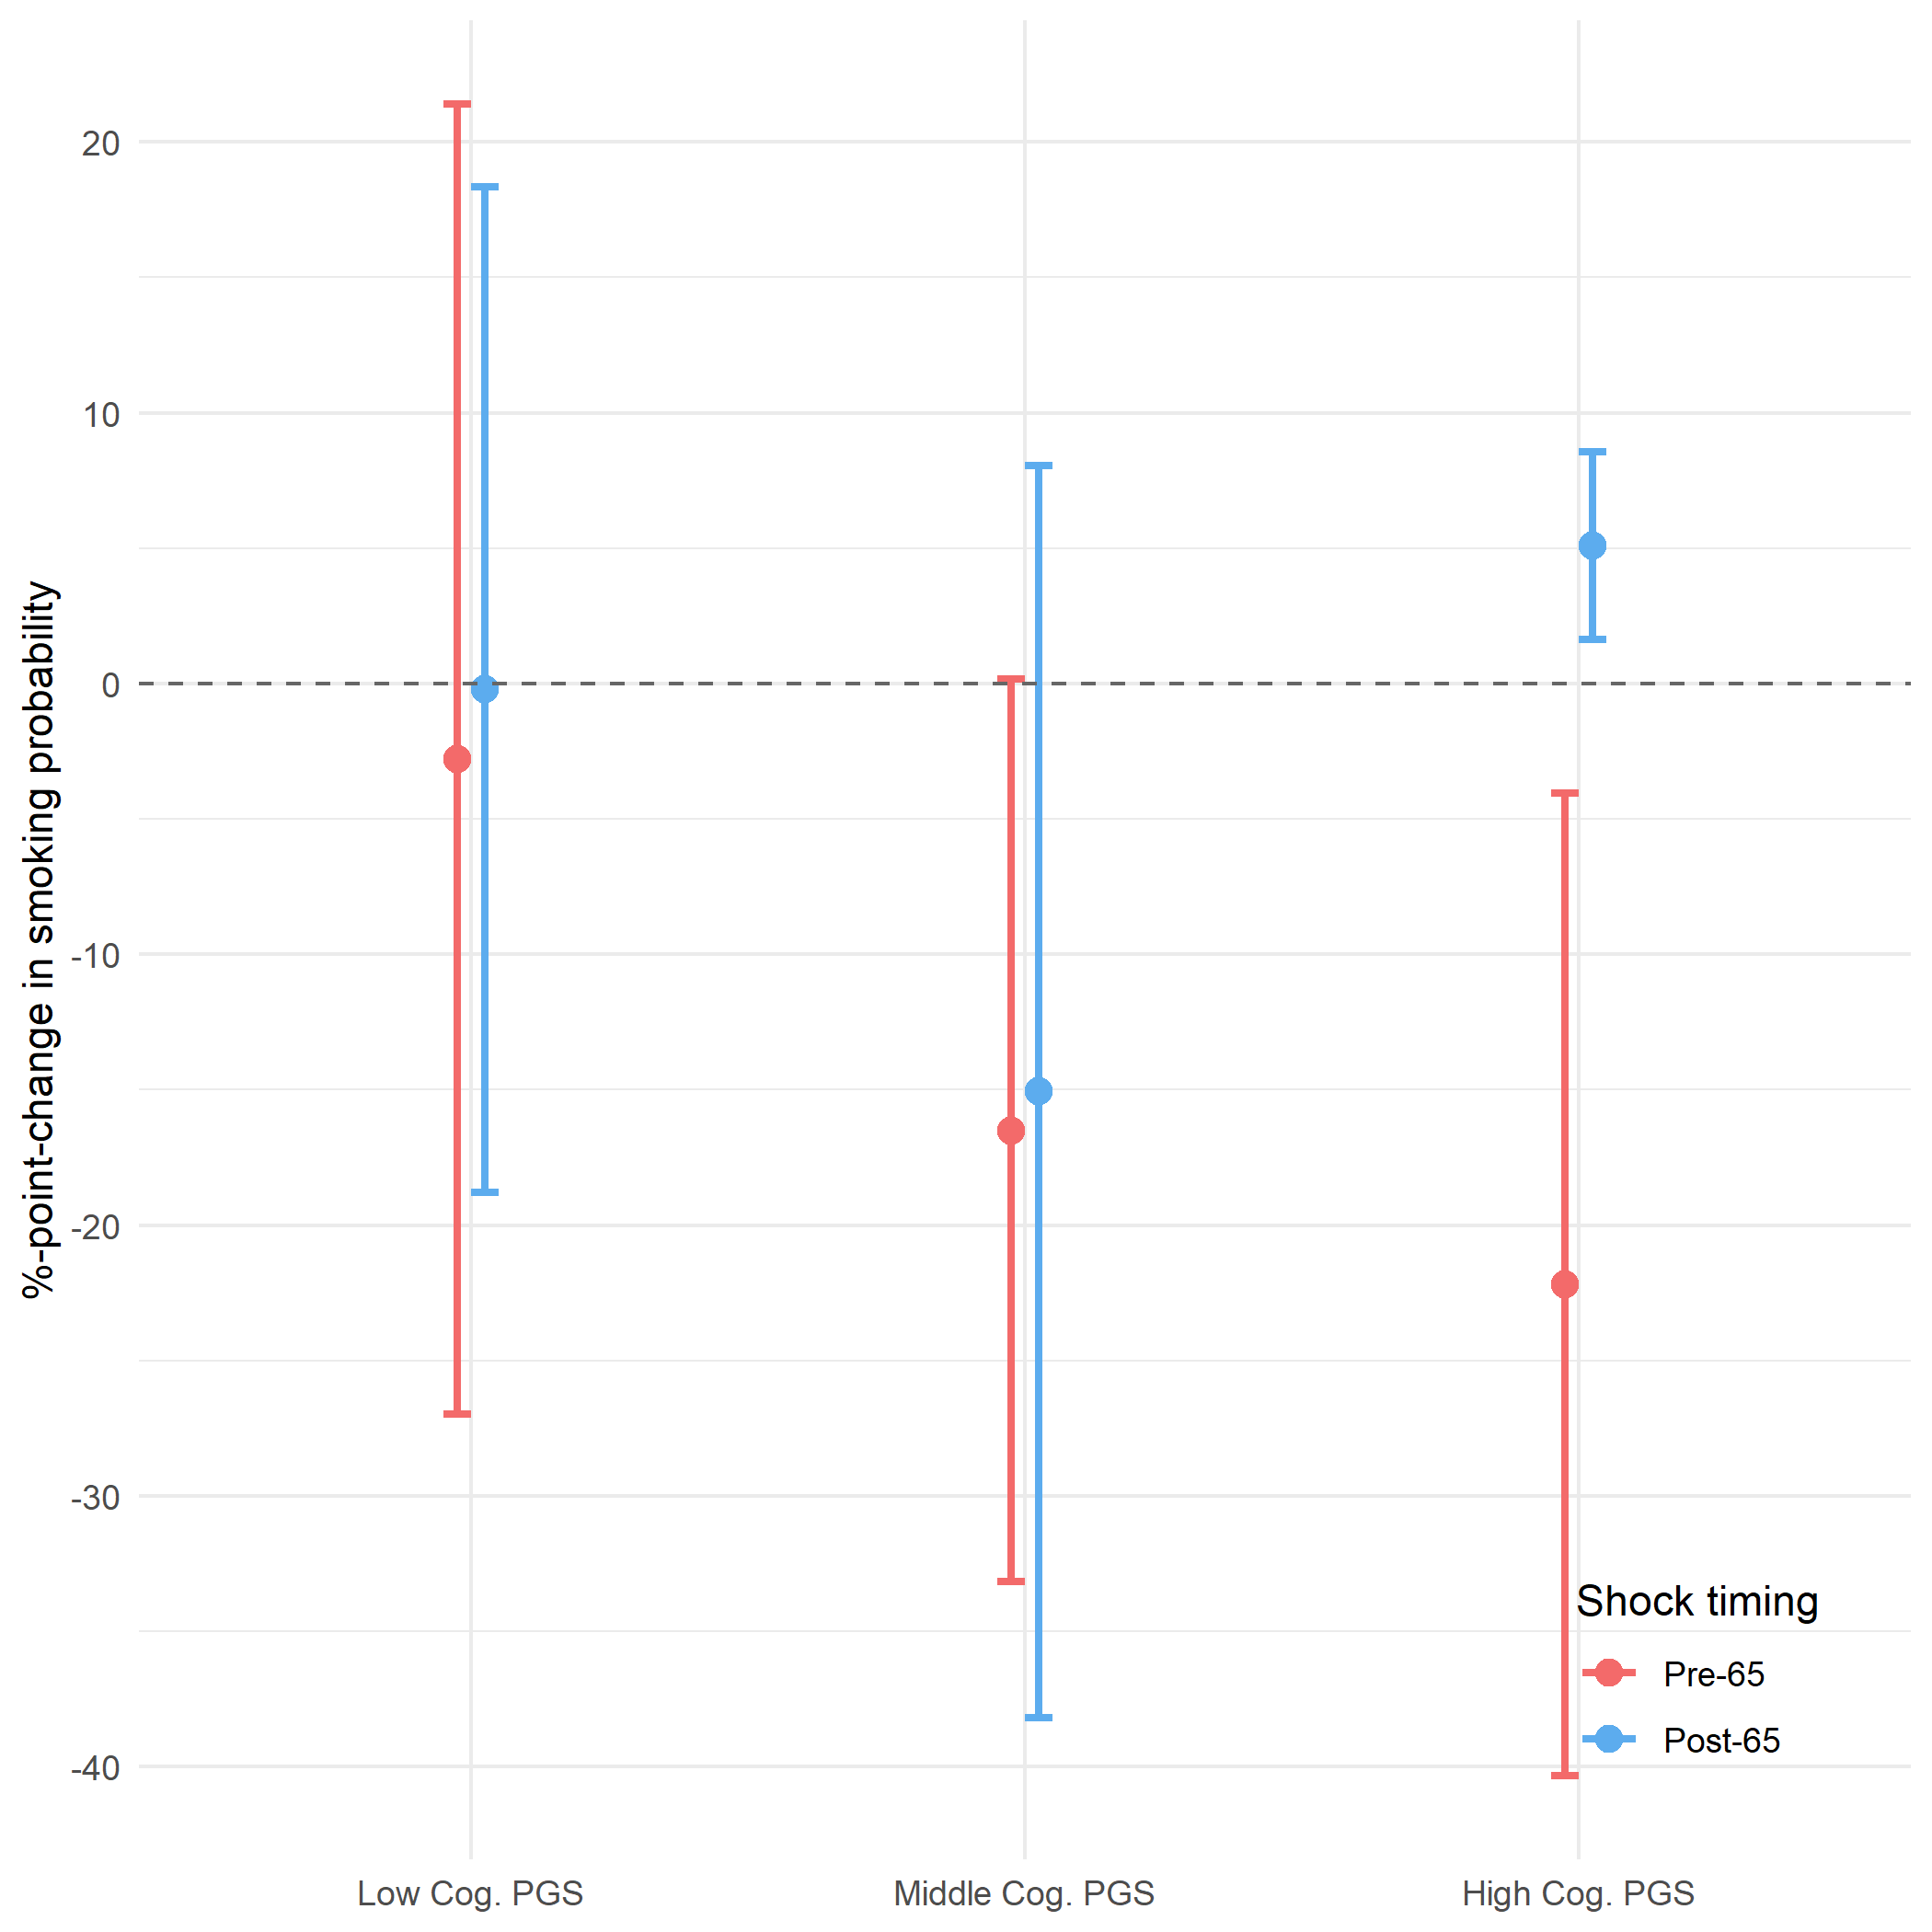
\includegraphics[width=0.3\textwidth]
		{../3_output/shock_effects/robustness_cogPGS_6070_100_cv.png}
		}
		\subfigure[\textsf{PGS for risk tolerance}]
		{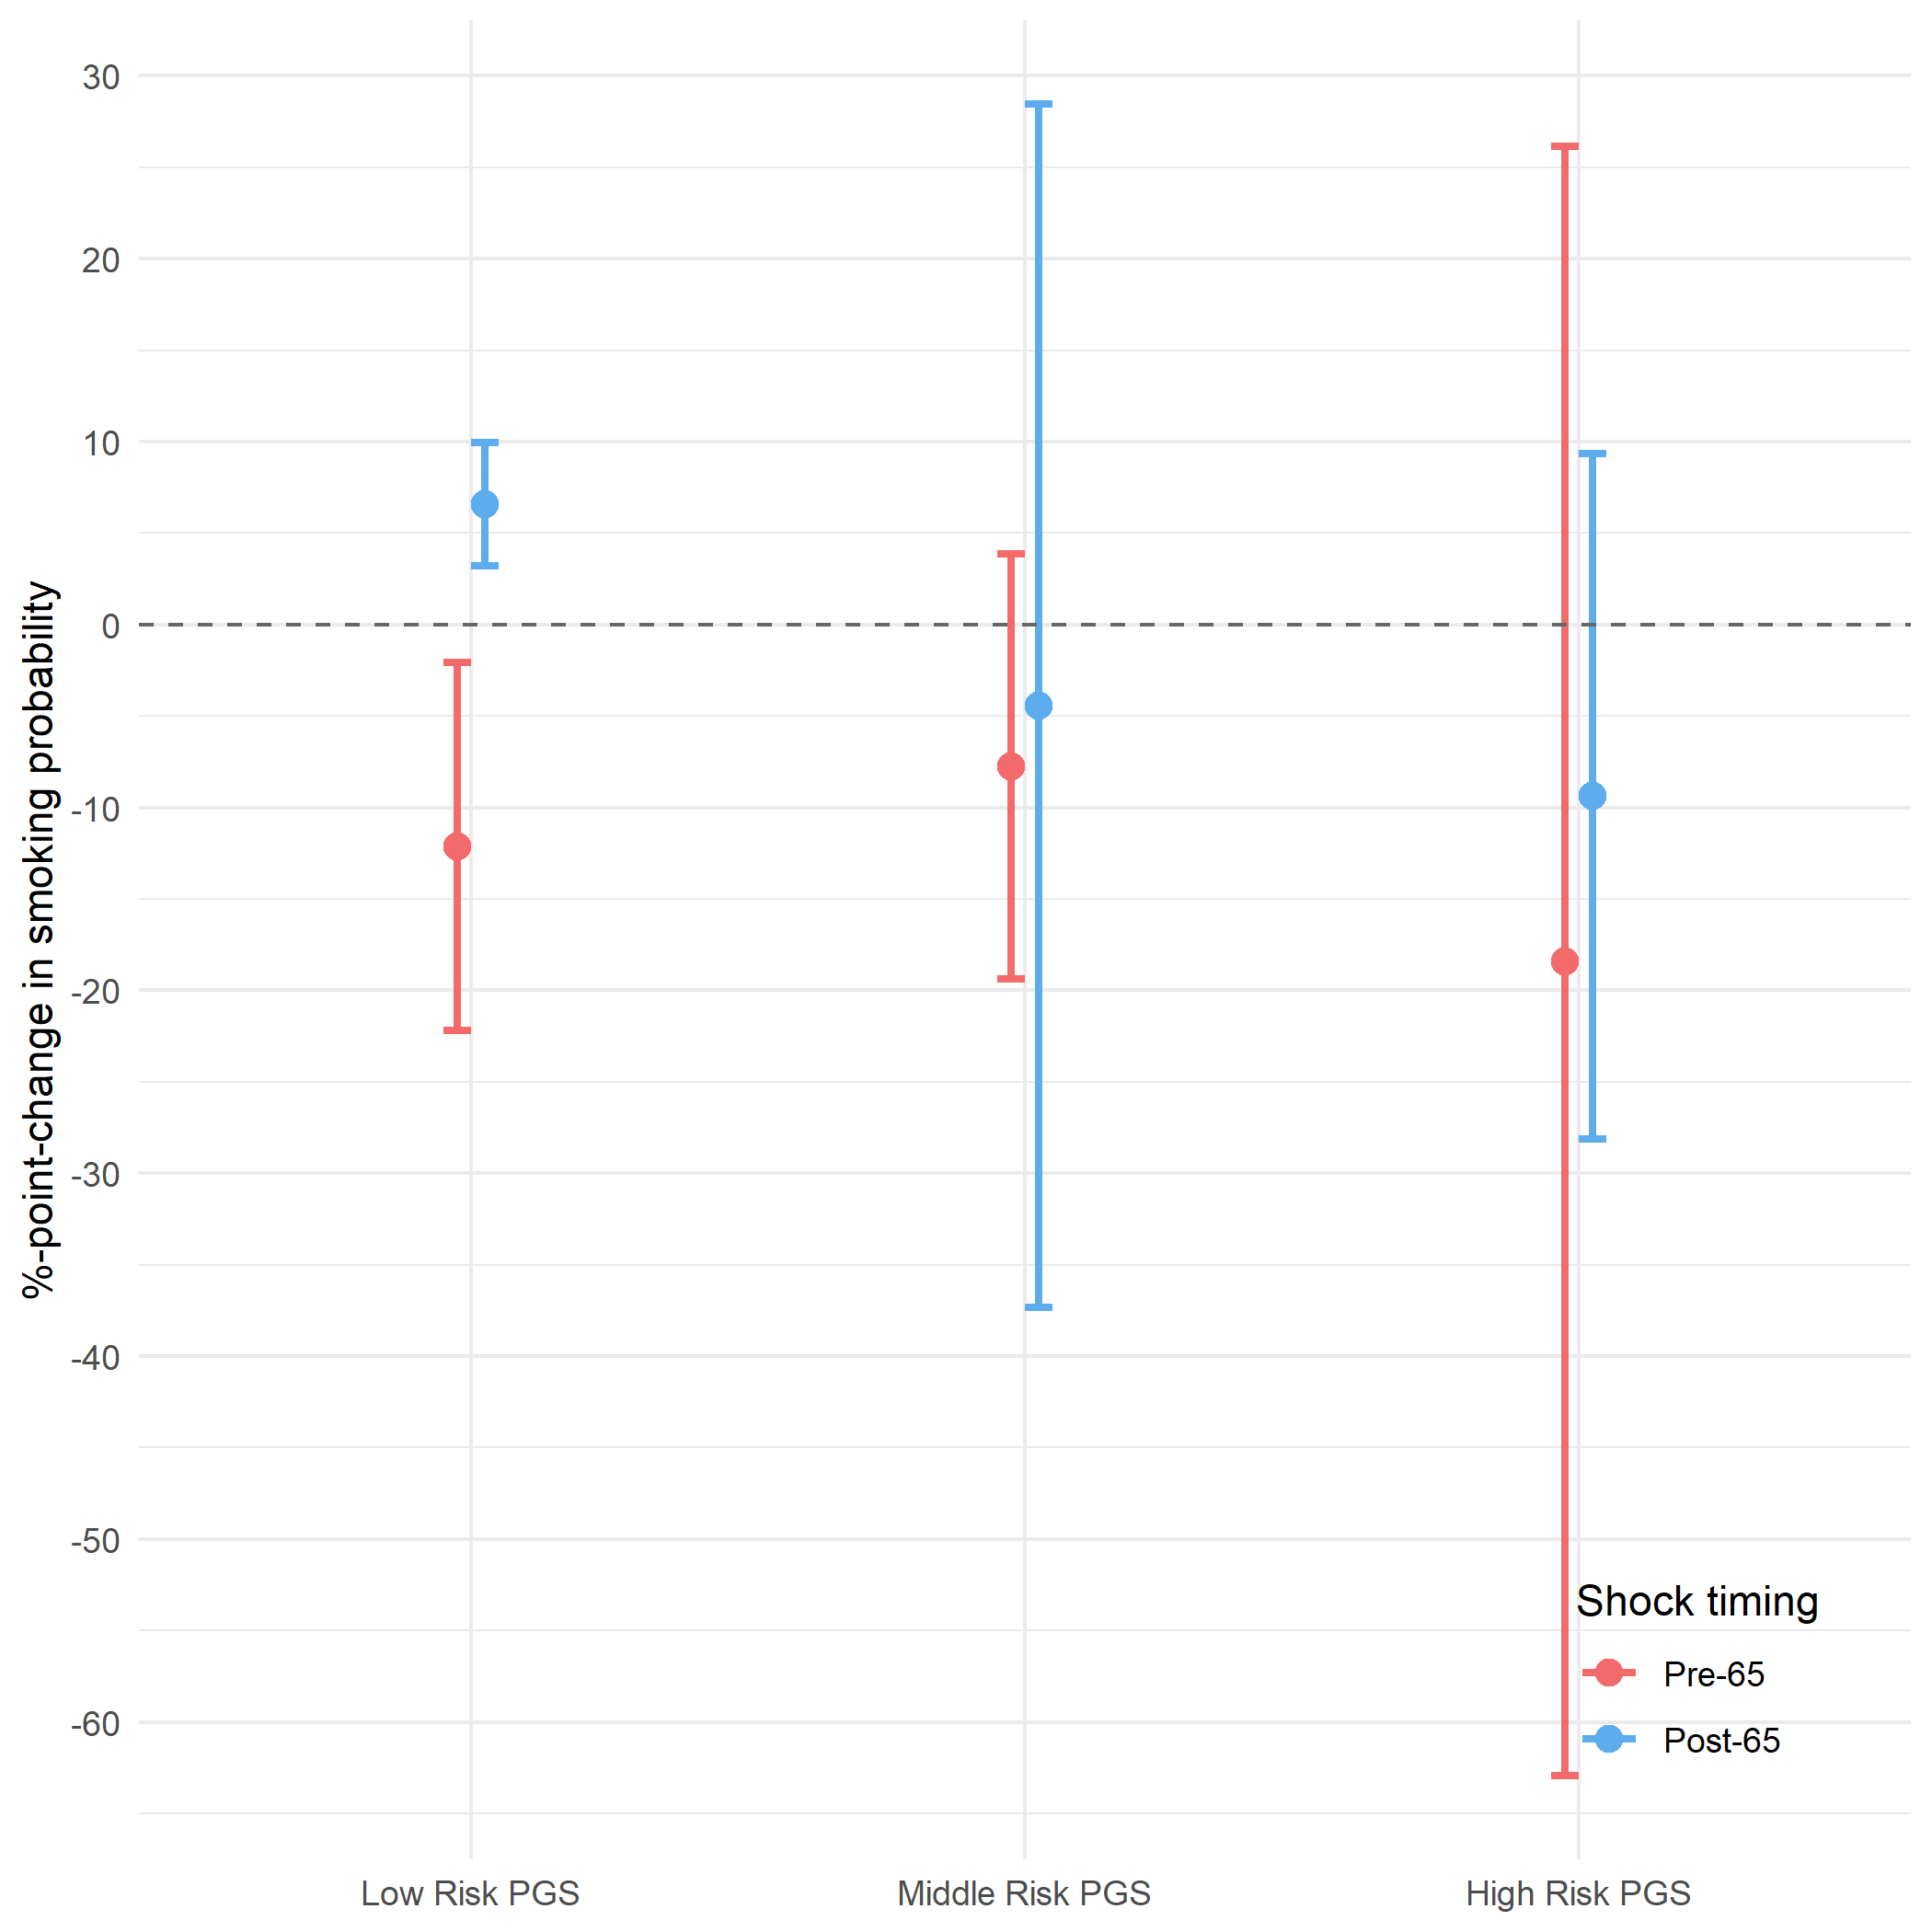
\includegraphics[width=0.3\textwidth]
		{../3_output/shock_effects/robustness_riskPGS_GWAS_6070_100_cv.png}
		}
		\subfigure[\textsf{PGS for non-cognitive skills}]
		{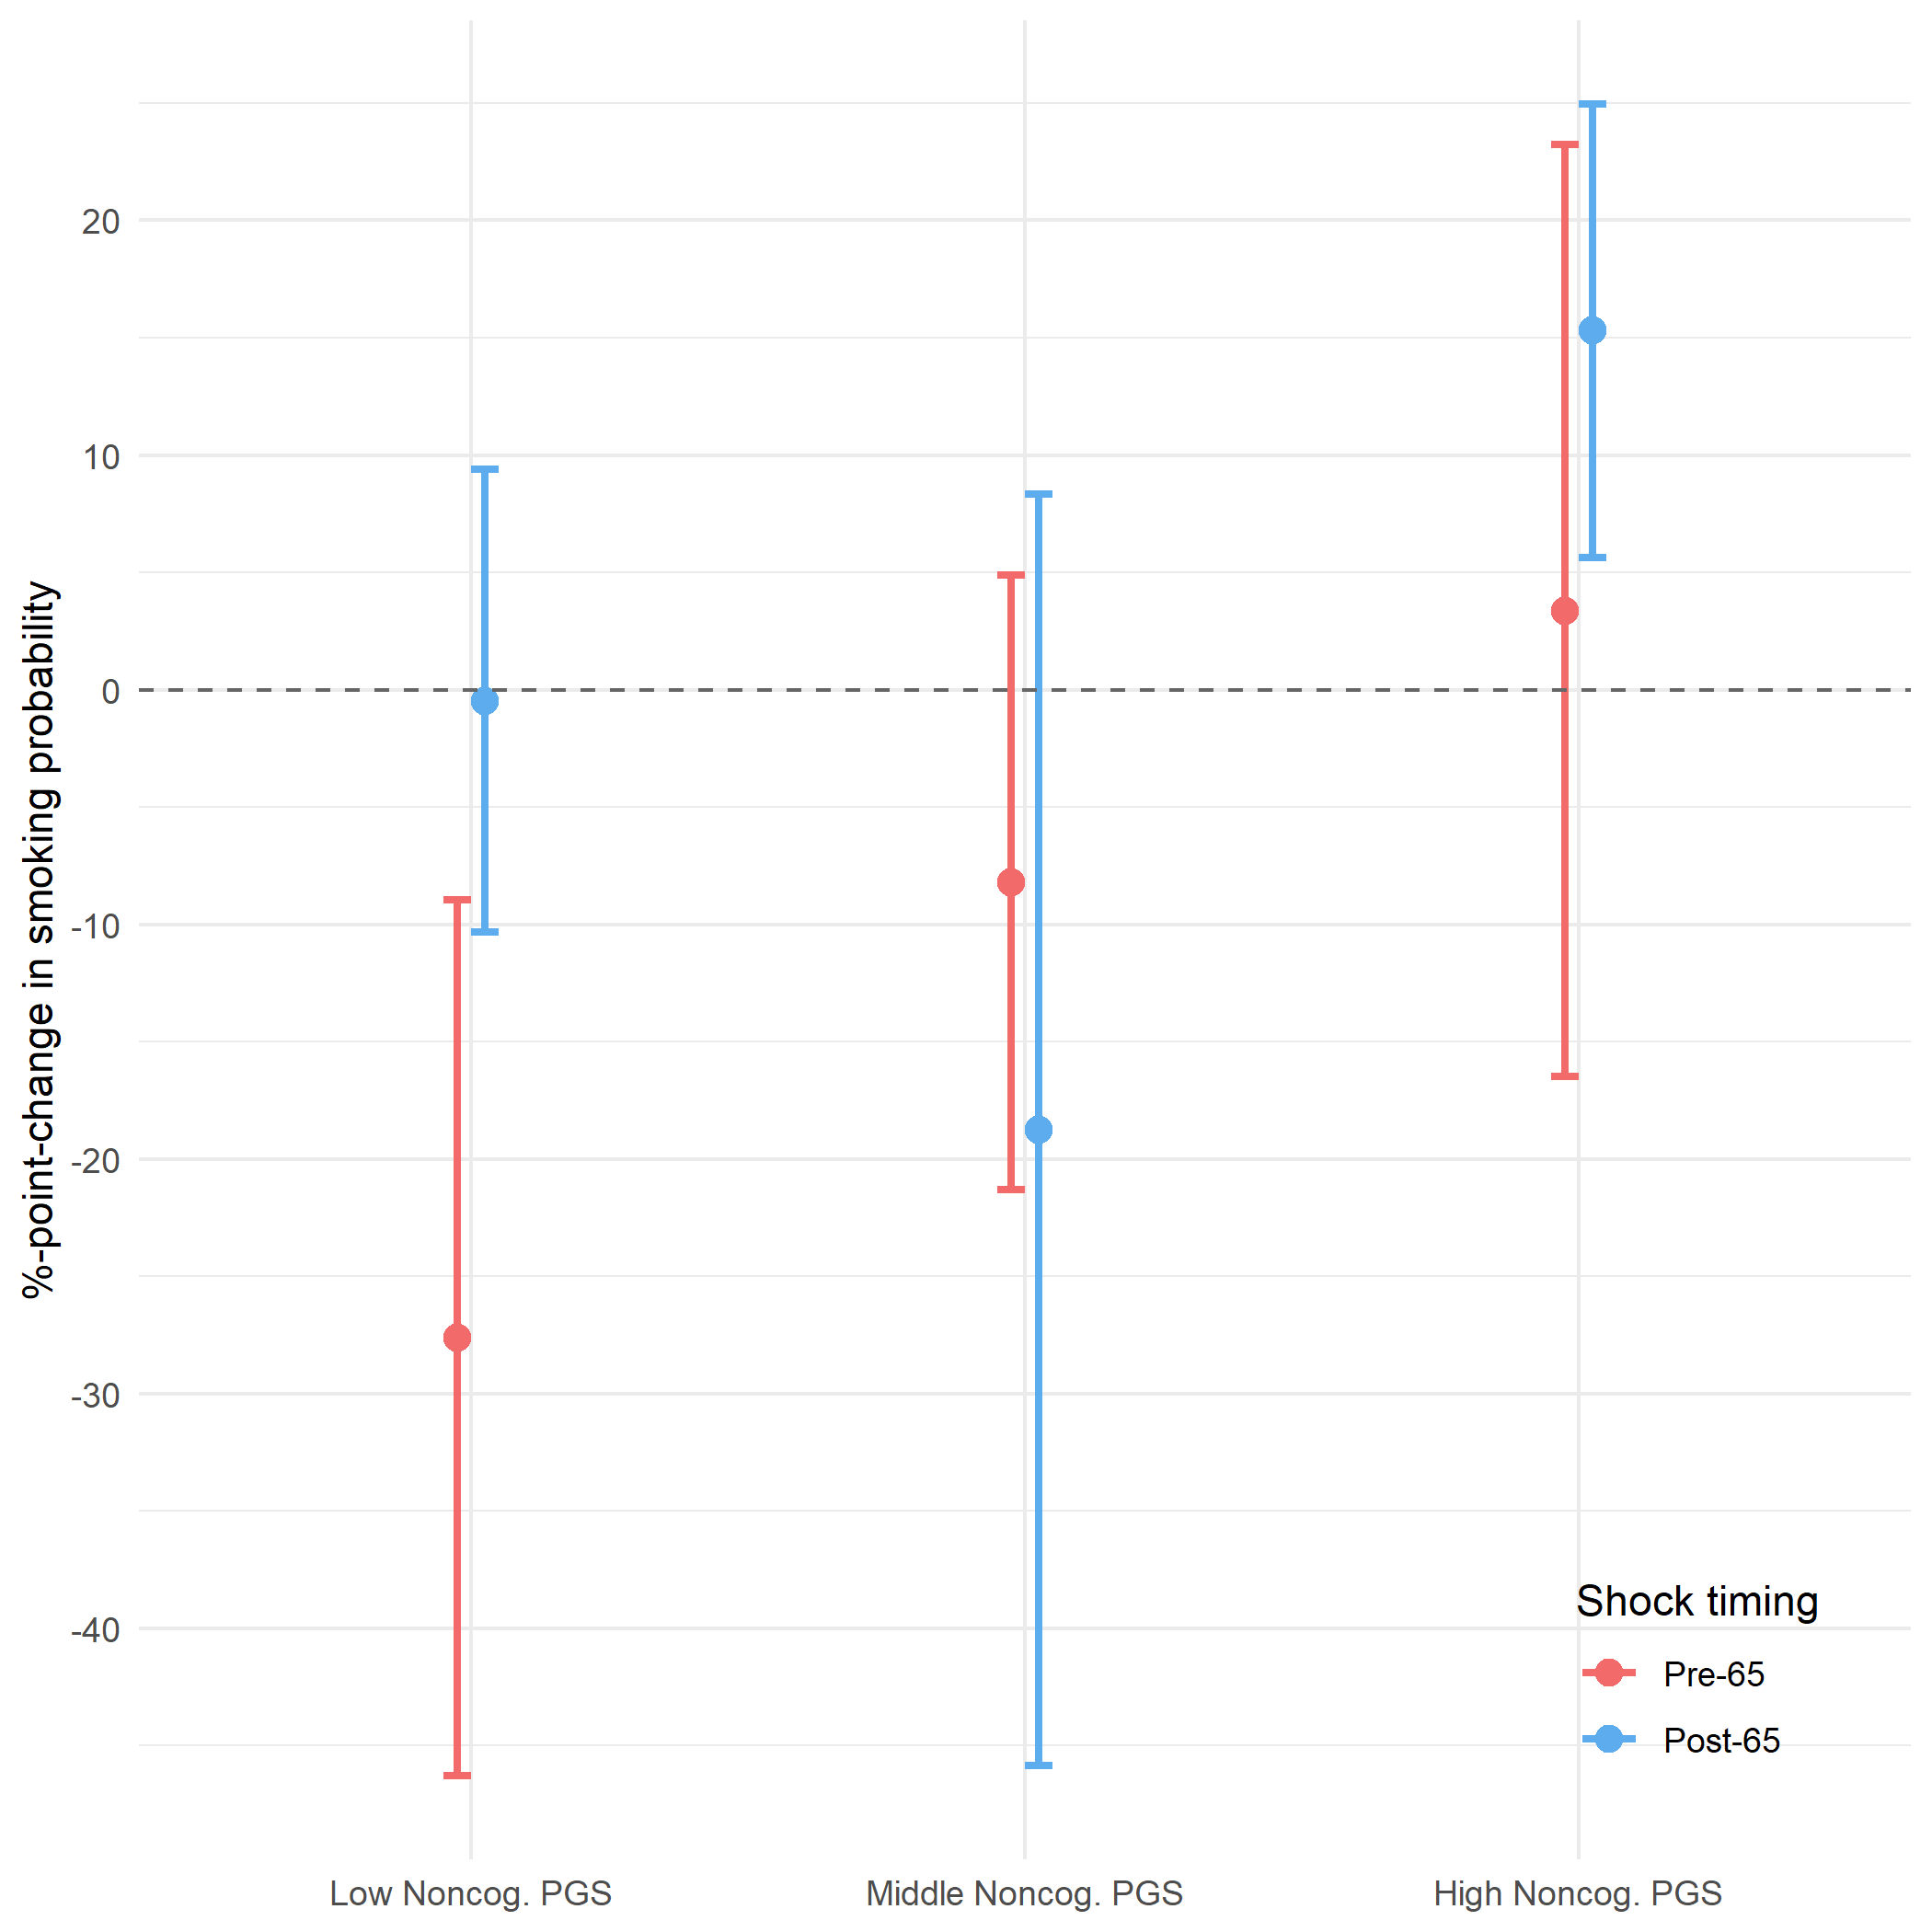
\includegraphics[width=0.3\textwidth]
		{../3_output/shock_effects/robustness_noncogPGS_6070_100_cv.png}
		}
		\subfigure[\textsf{PGS for BMI}]
		{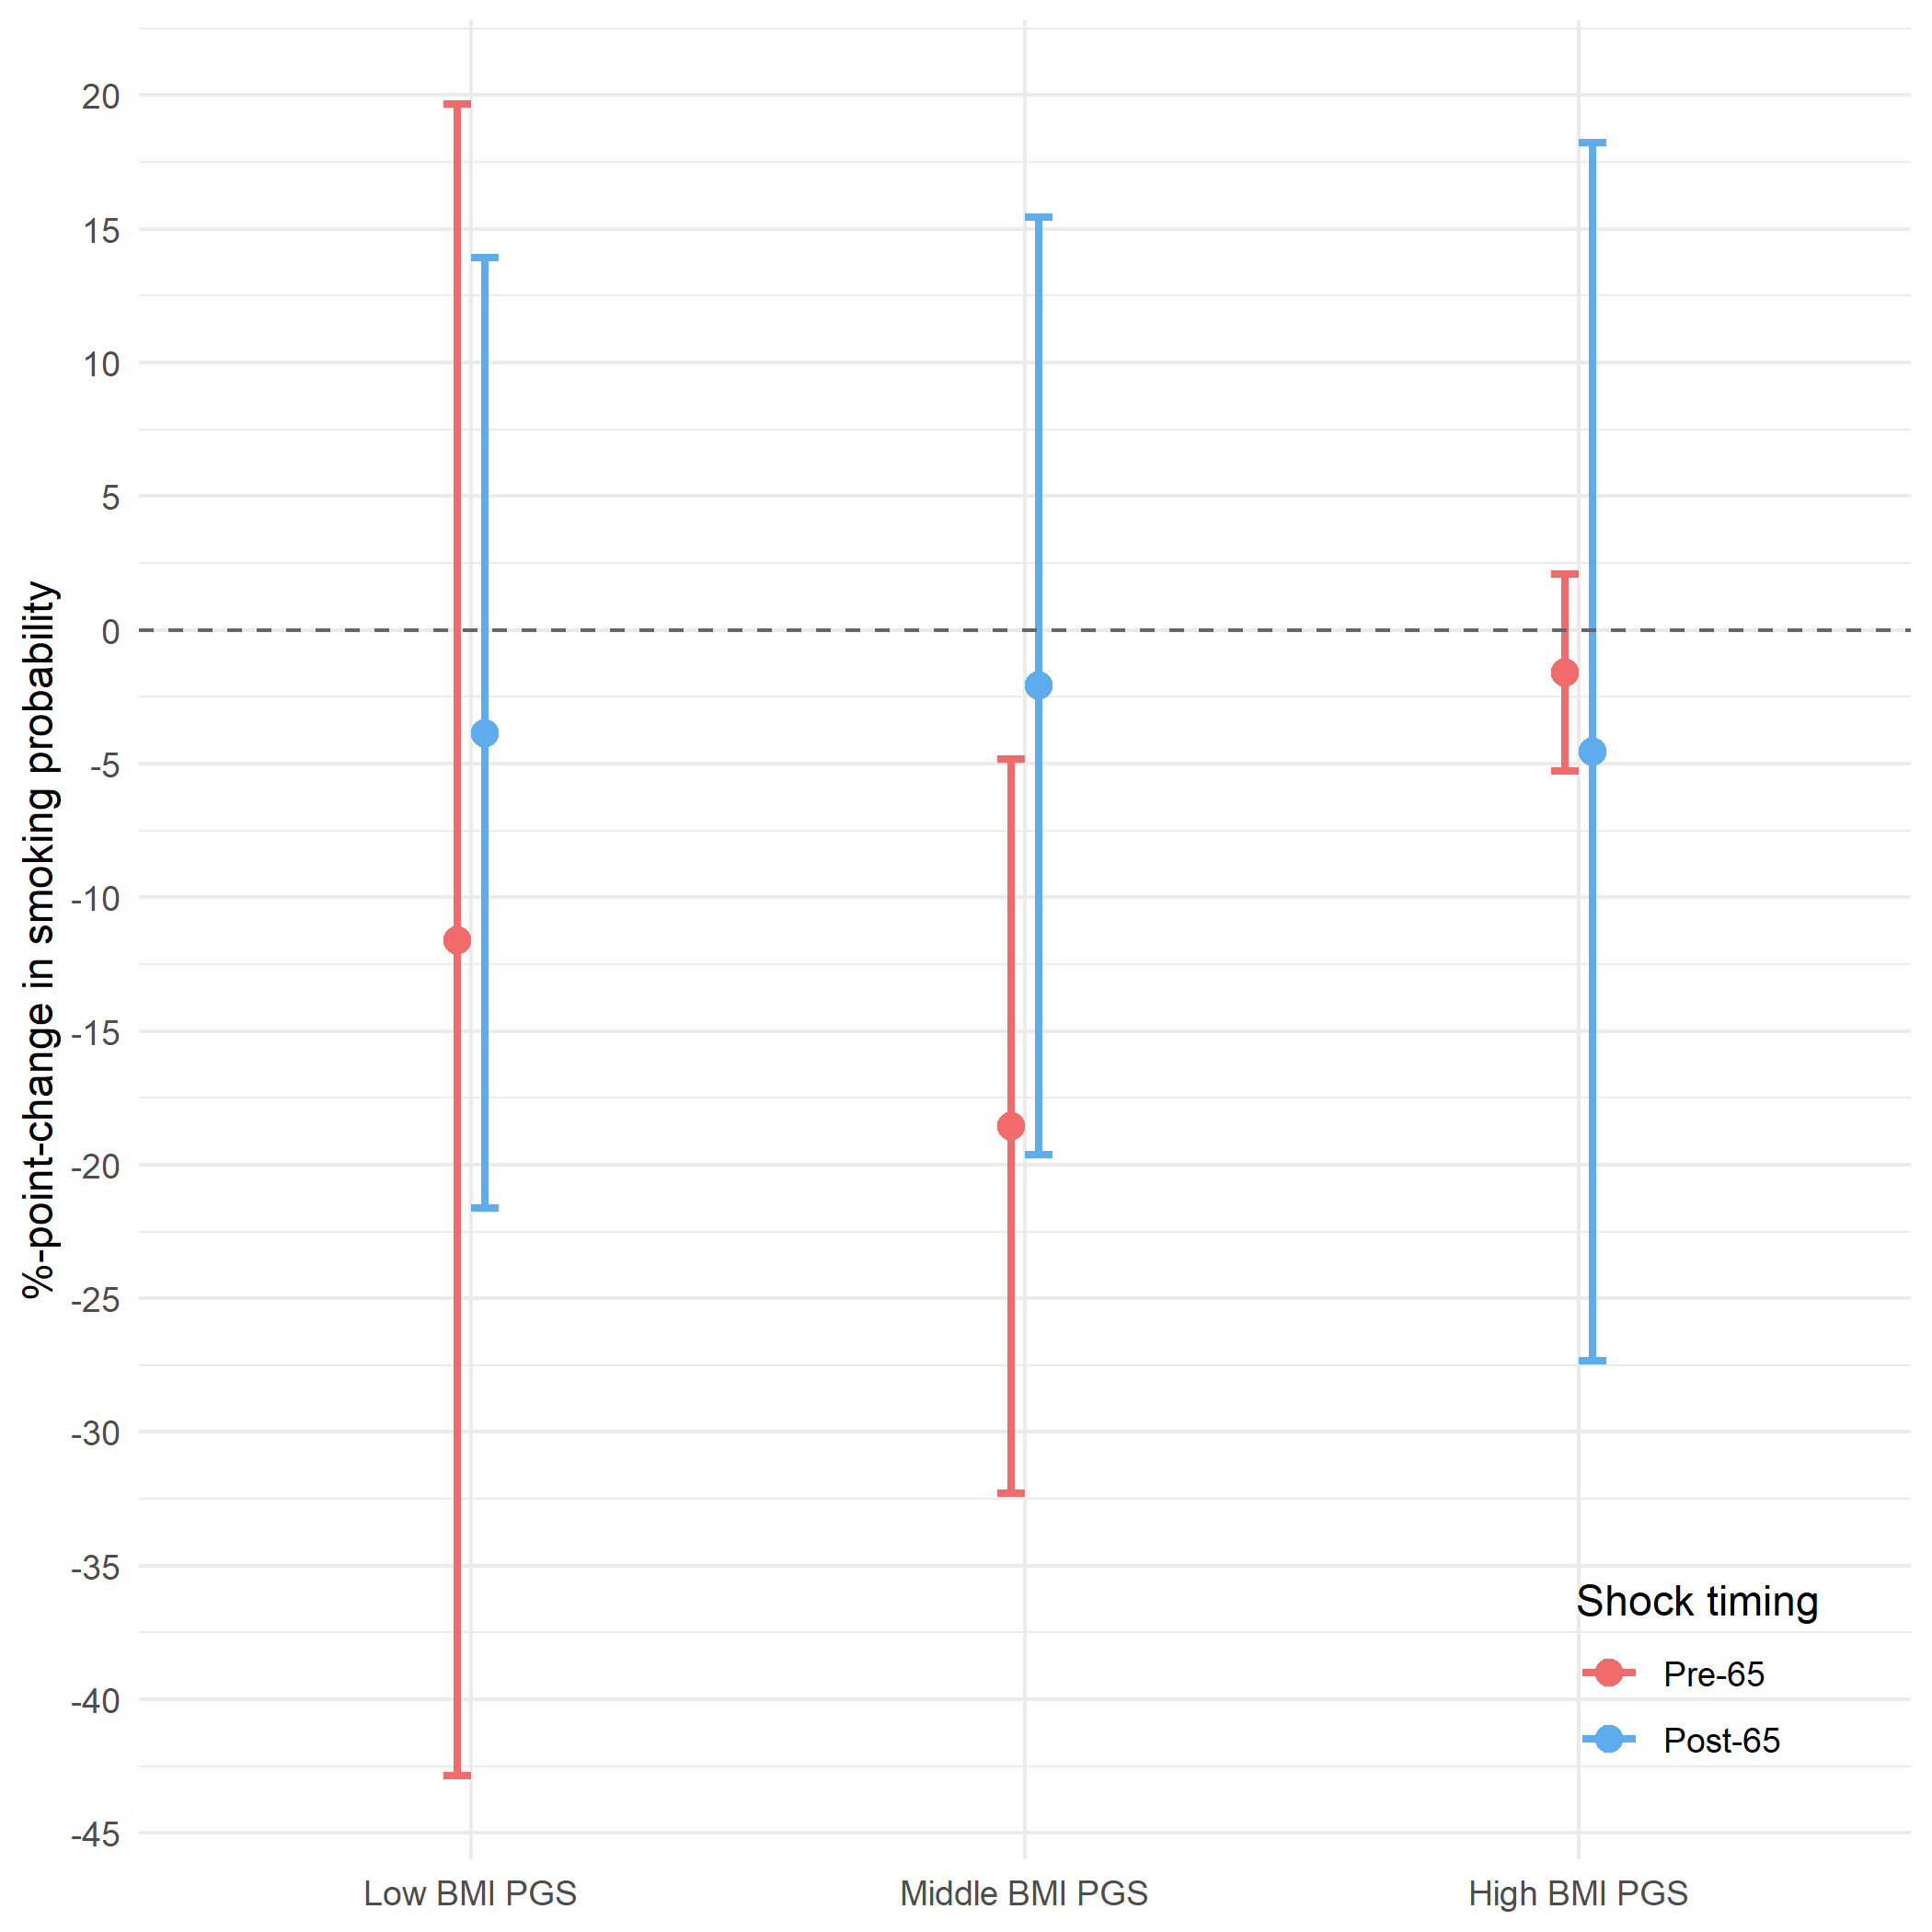
\includegraphics[width=0.3\textwidth]
		{../3_output/shock_effects/robustness_bmiPGS_6070_100_cv.png}
		}
		%
		\caption{Other Polygenic Scores as Proxy for Moral Hazard Heterogeneity
					\label{fig:otherPGS}}
	\vspace{-5ex}
	\floatfoot{
	\textit{Notes:}
	The figures report the effect of suffering a health shock on the probability of smoking for the pre-65 uninsured subgroup, stratified by timing of the shock (before and after the age of 65) and different polygenic scores.
	Pre-65: Health shock since the last survey reported at ages 60-64.
	Post-65: Health shock since the last survey reported at ages 67-70.
	Effects are estimated using a combination of the coefficients from equation \ref{eq:regression} where $g_i$ is replaced by the different polygenic scores reported in the sub-figure captions, following the derivation described in \ref{appsec:derivation}.
	Bars show 95\% confidence intervals, standard error clustered at the individual level.
	\\ \textit{Data used}: HRS study sample, n = 5,854.
	}
	\end{center}
\end{figure}

\clearpage
\subsubsection{Relaxing the Criteria for Inclusion in the Pre-65 Uninsured Group}
% Table created by stargazer v.5.2 by Marek Hlavac, Harvard University. E-mail: hlavac at fas.harvard.edu
\begin{table}[!ht]
	\centering
	\caption{Summary of Statistical Results for the Pre-65 Uninsured Subgroup (Using Different Definitions of the Pre-65 Uninsured Status Indicator)}
	%\label{suptab:65def}
	%\resizebox{\textwidth}{!}{
%	% latex table generated in R 4.0.2 by xtable 1.8-4 package
% 
\begin{tabular}{ l | p{2cm}p{2cm}| p{2cm}p{2cm}| p{2cm}p{2cm}}
  & \multicolumn{2}{c}{ \textit{100\% uninsured}} & \multicolumn{2}{c}{ \textit{75\% uninsured}} & \multicolumn{2}{c}{ \textit{50\% uninsured}} \\
 \toprule
  \multicolumn{7}{c}{ \textbf{Effect of health shock on smoking probability}} \\
 \midrule
 & Low PGS & High PGS & Low PGS & High PGS & Low PGS & High PGS \\ 
   \midrule
Pre 65 & -0.165** & -0.108 & -0.165** & -0.108 & -0.043 & -0.054 \\ 
   & (0.069) & (0.083) & (0.069) & (0.083) & (0.056) & (0.05) \\ 
  Post 65 & 0.09*** & -0.13 & 0.09*** & -0.13 & 0.07*** & -0.09 \\ 
   & (0.026) & (0.089) & (0.026) & (0.089) & (0.017) & (0.057) \\ 
   \toprule \multicolumn{7}{c}{ \textbf{Effect of health insurance on effect of health shock}} \\
 \midrule
 & Low PGS & High PGS & Low PGS & High PGS & Low PGS & High PGS \\ 
   \midrule
Post 65 - Pre 65 & 0.256*** & -0.023 & 0.256*** & -0.023 & 0.112* & -0.037 \\ 
   & (0.079) & (0.121) & (0.079) & (0.121) & (0.06) & (0.076) \\ 
   \toprule \multicolumn{7}{c}{ \textbf{Differential effect of health insurance by genetic group}} \\
 \midrule
 & High PGS  & - low PGS & High PGS  & - low PGS & High PGS  & - low PGS \\ 
   \midrule
Post 65 - Pre 65 & -0.279* &  & -0.279* &  & -0.149 &  \\ 
   & (0.144) &  & (0.144) &  & (0.096) &  \\ 
  \end{tabular}

	% latex table generated in R 4.0.2 by xtable 1.8-4 package
% 
\begin{tabular}{ l | p{2cm}p{2cm}| p{2cm}p{2cm}| p{2cm}p{2cm}}
  & \multicolumn{2}{c}{ \textit{100\% uninsured}} & \multicolumn{2}{c}{ \textit{66\% uninsured}} & \multicolumn{2}{c}{ \textit{33\% uninsured}} \\
 \toprule
  \multicolumn{7}{c}{ \textbf{Effect of health shock on smoking probability}} \\
 \midrule
 & Low PGS & High PGS & Low PGS & High PGS & Low PGS & High PGS \\ 
   \midrule
Pre 65 & -0.165** & -0.108 & -0.147** & -0.055 & -0.055 & -0.09* \\ 
   & (0.069) & (0.083) & (0.059) & (0.06) & (0.068) & (0.048) \\ 
  Post 65 & 0.09*** & -0.13 & 0.086*** & -0.091 & 0.052 & -0.102** \\ 
   & (0.026) & (0.089) & (0.021) & (0.078) & (0.036) & (0.05) \\ 
   \toprule \multicolumn{7}{c}{ \textbf{Effect of health insurance on effect of health shock}} \\
 \midrule
 & Low PGS & High PGS & Low PGS & High PGS & Low PGS & High PGS \\ 
   \midrule
Post 65 - Pre 65 & 0.256*** & -0.023 & 0.233*** & -0.036 & 0.107 & -0.012 \\ 
   & (0.079) & (0.121) & (0.067) & (0.098) & (0.076) & (0.069) \\ 
   \toprule \multicolumn{7}{c}{ \textbf{Differential effect of health insurance by genetic group}} \\
 \midrule
 & High PGS  & - low PGS & High PGS  & - low PGS & High PGS  & - low PGS \\ 
   \midrule
Post 65 - Pre 65 & -0.279* &  & -0.269** &  & -0.119 &  \\ 
   & (0.144) &  & (0.118) &  & (0.103) &  \\ 
  \end{tabular}

		\footnotesize
		\begin{flushleft}
		Main study results, for comparison.\\
		Pre-65 uninsured status indicator set to 1 for respondents who were uninsured in at least 66\% of all pre-65 observations.\\
		Pre-65 uninsured status indicator set to 1 for respondents who were uninsured in at least 33\% of all pre-65 observations.\\
		$^{*}$P $<$ 0.1; $^{**}$P $<$ 0.05; $^{***}$P $<$ 0.01. Robust standard errors in parentheses were clustered at the individual level.\\
		Low PGS = lowest tertile of the polygenic score distribution; high PGS = upper two tertiles of the polygenic score distribution.\\
		Pre-65: Health shock since the last survey reported at ages 60-64. Post-65: Health shock since the last survey reported at ages 67-70.\\
		\textit{Data used}: HRS study sample, n = 5,854.
		\end{flushleft}
%}
\end{table}

\clearpage
%\subsubsection{Expanding the Age Range}
%% Table created by stargazer v.5.2 by Marek Hlavac, Harvard University. E-mail: hlavac at fas.harvard.edu
%\begin{table}[ht] \centering
%	\vspace{-4mm}
%	\caption{Summary of Statistical Results for the Pre-65 Uninsured Subgroup (Using Different Age Range Restrictions in the study Sample)}
%	\label{suptab:Agedef}
%	\resizebox{\textwidth}{!}{
%	% latex table generated in R 4.0.2 by xtable 1.8-4 package
% 
\begin{tabular}{l| p{2cm}p{2cm}| p{2cm}p{2cm}| p{2cm}p{2cm}}
   & \multicolumn{2}{c}{ \textbf{60-70 years old}} & \multicolumn{2}{c}{ \textbf{59-71 years old}} & \multicolumn{2}{c}{ \textbf{58-72 years old}} \\
 \toprule
  \multicolumn{7}{c}{ \textbf{Effect of health shock on smoking probability}} \\
 \midrule
 & Low PGS & High PGS & Low PGS & High PGS & Low PGS & High PGS \\ 
   \midrule
Pre 65 & 0.125 & -0.322*** & 0.164 & -0.223* & 0.072 & -0.225* \\ 
   & (0.153) & (0.1) & (0.171) & (0.117) & (0.144) & (0.125) \\ 
  Post 65 & 0.065** & -0.047 & 0.089** & -0.025 & 0.174** & -0.023 \\ 
   & (0.029) & (0.074) & (0.039) & (0.077) & (0.068) & (0.077) \\ 
   \toprule \multicolumn{7}{c}{ \textbf{Effect of health insurance on effect of health shock}} \\
 \midrule
 & Low PGS & High PGS & Low PGS & High PGS & Low PGS & High PGS \\ 
   \midrule
Post 65 - Pre 65 & -0.06 & 0.275** & -0.076 & 0.198 & 0.102 & 0.202 \\ 
   & (0.153) & (0.123) & (0.173) & (0.141) & (0.156) & (0.147) \\ 
   \toprule \multicolumn{7}{c}{ \textbf{Differential effect of health insurance by genetic group}} \\
 \midrule
 & High PGS  & - low PGS & High PGS  & - low PGS & High PGS  & - low PGS \\ 
   \midrule
Post 65 - Pre 65 & 0.334* &  & 0.273 &  & 0.1 &  \\ 
   & (0.196) &  & (0.223) &  & (0.215) &  \\ 
   & Low PGS & High PGS & Low PGS & High PGS & Low PGS & High PGS \\ 
   \toprule & \multicolumn{2}{c}{ \textbf{60-70 years old}} & \multicolumn{2}{c}{ \textbf{55-70 years old}} & \multicolumn{2}{c}{ \textbf{60-75 years old}} \\
 \toprule \multicolumn{7}{c}{ \textbf{Effect of health shock on smoking probability}} \\
 \midrule
Pre 65 & 0.125 & -0.322*** & 0.022 & -0.133 & 0.012 & -0.205 \\ 
   \midrule
 & (0.153) & (0.1) & (0.114) & (0.153) & (0.053) & (0.141) \\ 
  Post 65 & 0.065** & -0.047 & 0.148** & -0.076 & 0.107** & -0.01 \\ 
   & (0.029) & (0.074) & (0.064) & (0.108) & (0.044) & (0.052) \\ 
   & Low PGS & High PGS & Low PGS & High PGS & Low PGS & High PGS \\ 
   \toprule \multicolumn{7}{c}{ \textbf{Effect of health insurance on effect of health shock}} \\
 \midrule
Post 65 - Pre 65 & -0.06 & 0.275** & 0.126 & 0.057 & 0.095 & 0.196 \\ 
   \midrule
 & (0.153) & (0.123) & (0.125) & (0.191) & (0.077) & (0.148) \\ 
   & High PGS  & - low PGS & High PGS  & - low PGS & High PGS  & - low PGS \\ 
   \toprule \multicolumn{7}{c}{ \textbf{Differential effect of health insurance by genetic group}} \\
 \midrule
Post 65 - Pre 65 & 0.334* &  & -0.068 &  & 0.101 &  \\ 
   \midrule
 & (0.196) &  & (0.228) &  & (0.167) &  \\ 
  \end{tabular}

%	}
%			\begin{flushleft}
%			\textsuperscript{a}Main study results, for comparison.\\
%			$^{*}$P $<$ 0.1; $^{**}$P $<$ 0.05; $^{***}$P $<$ 0.01. Robust standard errors in parentheses were clustered at the individual level.\\
%			Low PGS = lowest tertile of the polygenic score distribution; high PGS = upper two tertiles of the polygenic score distribution.\\
%			Pre-65: Health shock since the last survey reported at ages 60-64. Post-65: Health shock since the last survey reported at ages 67-70.\\
%			\textit{Data used}: study sample, but changing the age limits used in Step 1 in Section \ref{supsubsec:reshape}.
%			\end{flushleft}
%
%\end{table}
%


\subsubsection{Including Individuals with Shocks Reported at Ages 65 and 66}
%\captionsetup{width = 12.5cm}
% Table created by stargazer v.5.2 by Marek Hlavac, Harvard University. E-mail: hlavac at fas.harvard.edu
\begin{table}[ht] \centering
	\vspace{-4mm}
	\caption{Summary of Statistical Results for the Pre-65 Uninsured Subgroup (Including Individuals Reporting a Health Shock when Aged 65 or 66 in the study Sample)}
	\label{suptab:6566}
	\vspace{4mm}
	%\resizebox{0.8\textwidth}{!}{
	% latex table generated in R 4.0.2 by xtable 1.8-4 package
% 
\begin{tabular}{l| p{3cm}p{3cm}| p{3cm}p{3cm}}
  & \multicolumn{2}{c}{ \textit{Analytic Sample}} & \multicolumn{2}{c}{ \textit{Including reported at 65/66}} \\
 \toprule
  \multicolumn{5}{c}{ \textbf{Effect of health shock on smoking probability}} \\
 \midrule
 & Low PGS & High PGS & Low PGS & High PGS \\ 
   \midrule
Pre 65 & -0.167** & -0.108 & -0.168** & -0.113 \\ 
   & (0.069) & (0.083) & (0.069) & (0.083) \\ 
  Post 65 & 0.089*** & -0.115 & 0.092*** & -0.184** \\ 
   & (0.024) & (0.093) & (0.026) & (0.085) \\ 
   \toprule \multicolumn{5}{c}{ \textbf{Effect of health insurance on effect of health shock}} \\
 \midrule
 & Low PGS & High PGS & Low PGS & High PGS \\ 
   \midrule
Post 65 - Pre 65 & 0.256*** & -0.008 & 0.26*** & -0.071 \\ 
   & (0.079) & (0.124) & (0.08) & (0.118) \\ 
   \toprule \multicolumn{5}{c}{ \textbf{Differential effect of health insurance by genetic group}} \\
 \midrule
 & High PGS  & - low PGS & High PGS  & - low PGS \\ 
   \midrule
Post 65 - Pre 65 & -0.264* &  & -0.331** &  \\ 
   & (0.146) &  & (0.142) &  \\ 
  \end{tabular}

			\begin{flushleft}
				Main study results, for comparison.\\
				study sample additionally includes individuals who reported experiencing a health shock since the last survey wave when interviewed at ages 65 or 66.\\
				$^{*}$P $<$ 0.1; $^{**}$P $<$ 0.05; $^{***}$P $<$ 0.01. Robust standard errors in parentheses were clustered at the individual level.\\
				Low PGS = lowest tertile of the polygenic score distribution; high PGS = upper two tertiles of the polygenic score distribution.\\
				Pre-65: Health shock since the last survey reported at ages 60-64. Post-65: Health shock since the last survey reported at ages 67-70.\\
				\textit{Data used}: study sample, but skipping Step 6 in Section \ref{supsubsec:reshape}.
				\vspace{5mm}
			\end{flushleft}
%	}
\end{table}


\pagebreak
\newpage

\subsubsection{Using Medicare Enrollment Status instead of age 65}
\label{supsec:robustness_enrollment}
Medicare enrollment refers to the RAND variable {\tt GOVMR}, which indicates whether the respondent is covered by Medicare in a given wave. For details on the survey questions and construction of this variable, see the RAND HRS documentation. %XXX\cite{RANDVersionP} (p. 1195ff.).\\


%\captionsetup{width = 10.2cm}
% Table created by stargazer v.5.2 by Marek Hlavac, Harvard University. E-mail: hlavac at fas.harvard.edu
% Date and time: Do, Apr 26, 2018 - 12:58:22
\begin{table}[!ht] \centering
	\caption{Summary of Statistical Results for the Pre-65 Uninsured Subgroup (Using Medicare Enrollment Status Instead of Medicare Eligibility Status)}
	\label{suptab:main_effects_medicare}
	%\resizebox{7.5cm}{!}{
% latex table generated in R 4.0.2 by xtable 1.8-4 package
% 
\begin{tabular}{lll}
  \toprule
  \multicolumn{3}{c}{ \textbf{Effect of health shock on smoking probability}} \\
 \midrule
 & Low PGS & High PGS \\ 
   \midrule
Without Medicare & -0.136** & -0.109 \\ 
   & (0.066) & (0.083) \\ 
  With Medicare & 0.097*** & -0.124 \\ 
   & (0.028) & (0.089) \\ 
   \toprule \multicolumn{3}{c}{ \textbf{Effect of health insurance on effect of health shock}} \\
 \midrule
 & Low PGS & High PGS \\ 
   \midrule
With - Without Medicare & 0.233*** & -0.016 \\ 
   & (0.077) & (0.121) \\ 
   \toprule \multicolumn{3}{c}{ \textbf{Differential effect of health insurance by genetic group}} \\
 \midrule
 & High PGS  & - low PGS \\ 
   \midrule
With - Without Medicare & -0.248* &  \\ 
   & (0.144) &  \\ 
  \end{tabular}

		\begin{flushleft}
			$^{*}$P $<$ 0.1; $^{**}$P $<$ 0.05; $^{***}$P $<$ 0.01. Robust standard errors in parentheses, clustered at the individual level.
			Low PGS = lowest tertile of the polygenic score distribution; high PGS = upper two tertiles of the polygenic score distribution.
			Effects are estimated using the coefficients in Table \ref{tab:reg_results_multi} and following the derivation described in \ref{appsec:derivation}, but replacing the post-65 indicator with Medicare enrollment status.
			%Composition of all effects as shown in Tables \ref{suptab:main_explained}, \ref{suptab:main_explained2}, and \ref{suptab:main_explained3}, but replacing the post-65 indicator with Medicare enrollment status.
			\textit{Data used}: HRS study sample with the additional restriction of a non-missing Medicare enrollment status.
		\end{flushleft}

	%\headrule
\end{table}


\subsection{Confounders} \label{appsec:confounders}
Tables \ref{suptab:placebo_1}-\ref{suptab:placebo_mortality} report the results for the effect of the shock on potential confounding variables.

\begin{table} \centering
	\caption{Summary of Placebo Checks for the Pre-65 Uninsured Subgroup for Income and Wealth}
	\label{suptab:placebo_1}
	\resizebox{\textwidth}{!}{
	% latex table generated in R 4.0.2 by xtable 1.8-4 package
% 
\begin{tabular}{l| p{2.5cm}p{2.5cm}| p{2.5cm}p{2.5cm}| p{2.5cm}p{2.5cm}}
  & \multicolumn{6}{c}{\textbf{Effect of health shock on...}} \\
 \toprule
  & \multicolumn{2}{c}{ \textbf{...individual earnings}} &  \multicolumn{2}{c}{ \textbf{...household earnings}} &  \multicolumn{2}{c}{ \textbf{...household wealth}}  \\
 \midrule
 & Low PGS & High PGS & Low PGS & High PGS & Low PGS & High PGS \\ 
   \midrule
Pre 65 & 0.416 & -0.145 & 0.391 & -0.368 & -5.429 & -1.669 \\ 
   & (2.782) & (1.178) & (0.75) & (0.744) & (3.858) & (2.021) \\ 
  Post 65 & 0.367 & 0.309 & -0.094 & 0.333 & -3.372 & 1.25 \\ 
   & (1.232) & (0.765) & (0.139) & (0.497) & (2.184) & (1.12) \\ 
   \toprule & \multicolumn{6}{c}{ \textbf{Effect of health insurance on effect of health shock}} \\
 \midrule
 & Low PGS & High PGS & Low PGS & High PGS & Low PGS & High PGS \\ 
   \midrule
Post 65 - Pre 65 & -0.049 & 0.454 & -0.485 & 0.701 & 2.057 & 2.919 \\ 
   & (3.065) & (1.424) & (0.789) & (0.902) & (4.442) & (2.325) \\ 
   \toprule & \multicolumn{6}{c}{ \textbf{Differential effect of health insurance by genetic group}} \\
 \midrule
 & High PGS  & - low PGS & High PGS  & - low PGS & High PGS  & - low PGS \\ 
   \midrule
Post 65 - Pre 65 & 0.503 &  & 1.186 &  & 0.862 &  \\ 
   & (3.379) &  & (1.2) &  & (5.014) &  \\ 
  \end{tabular}
}
\end{table}

\begin{table} \centering
	\caption{Summary of Placebo Checks for the Pre-65 Uninsured Subgroup for Retirement, Relationship Status and Out-of-Pocket Medical Expenditures}
	\label{suptab:placebo_2}
	\resizebox{\textwidth}{!}{
		% latex table generated in R 4.0.2 by xtable 1.8-4 package
% 
\begin{tabular}{l| p{2.5cm}p{2.5cm}| p{2.5cm}p{2.5cm}| p{2.5cm}p{2.5cm}}
  & \multicolumn{6}{c}{\textbf{Effect of health shock on...}} \\
 \toprule
  & \multicolumn{2}{c}{ \textbf{...retirement}} &  \multicolumn{2}{c}{ \textbf{...relationship status}} &  \multicolumn{2}{c}{ \textbf{...OOP medical expenditures}}  \\
 \midrule
 & Low PGS & High PGS & Low PGS & High PGS & Low PGS & High PGS \\ 
   \midrule
Pre 65 & 0.212 & 0.094 & 0.081 & 0.044 & 2.384*** & 1.607*** \\ 
   & (0.265) & (0.093) & (0.073) & (0.063) & (0.736) & (0.571) \\ 
  Post 65 & 0.015 & 0.022 & 0.01 & 0.041 & 0.26 & -1.27 \\ 
   & (0.093) & (0.13) & (0.01) & (0.04) & (0.658) & (0.873) \\ 
   \toprule & \multicolumn{6}{c}{ \textbf{Effect of health insurance on effect of health shock}} \\
 \midrule
 & Low PGS & High PGS & Low PGS & High PGS & Low PGS & High PGS \\ 
   \midrule
Post 65 - Pre 65 & -0.197 & -0.071 & -0.071 & -0.003 & -2.123** & -2.878*** \\ 
   & (0.28) & (0.16) & (0.07) & (0.074) & (1.008) & (1.056) \\ 
   \toprule & \multicolumn{6}{c}{ \textbf{Differential effect of health insurance by genetic group}} \\
 \midrule
 & High PGS  & - low PGS & High PGS  & - low PGS & High PGS  & - low PGS \\ 
   \midrule
Post 65 - Pre 65 & 0.125 &  & 0.068 &  & -0.754 &  \\ 
   & (0.322) &  & (0.102) &  & (1.457) &  \\ 
  \end{tabular}
}
\end{table}

\begin{table} \centering
	\caption{Summary of Placebo Checks for the Pre-65 Uninsured Subgroup for Mortality within 2 and 5 years}
	\label{suptab:placebo_mortality}
	\resizebox{\textwidth}{!}{
		% latex table generated in R 4.0.2 by xtable 1.8-4 package
% 
\begin{tabular}{l| p{2.5cm}p{2.5cm}| p{2.5cm}p{2.5cm}}
  & \multicolumn{4}{c}{\textbf{Effect of health shock on mortality within...}} \\
 \toprule
  & \multicolumn{2}{c}{ \textbf{...2 years}} &  \multicolumn{2}{c}{ \textbf{...5 years}}  \\
 \midrule
 & Low PGS & High PGS & Low PGS & High PGS \\ 
   \midrule
Pre 65 & 0.004 & 0.015 & -0.046 & -0.113 \\ 
   & (0.015) & (0.09) & (0.061) & (0.119) \\ 
  Post 65 & -0.001 & -0.074 & 0.204 & 0.009 \\ 
   & (0.011) & (0.065) & (0.179) & (0.103) \\ 
   \toprule & \multicolumn{4}{c}{ \textbf{Effect of health insurance on effect of health shock}} \\
 \midrule
 & Low PGS & High PGS & Low PGS & High PGS \\ 
   \midrule
Post 65 - Pre 65 & -0.005 & -0.089 & 0.25 & 0.122 \\ 
   & (0.025) & (0.113) & (0.191) & (0.154) \\ 
   \toprule & \multicolumn{4}{c}{ \textbf{Differential effect of health insurance by genetic group}} \\
 \midrule
 & High PGS  & - low PGS & High PGS  & - low PGS \\ 
   \midrule
Post 65 - Pre 65 & -0.085 &  & -0.129 &  \\ 
   & (0.116) &  & (0.245) &  \\ 
  \end{tabular}
}
\end{table}



\end{document}
